
\RequirePackage{fix-cm}

% Document Settings
\documentclass[natbib,twocolumn]{svjour3}


% Flushing
\smartqed


% Packages
\usepackage{graphicx}
%\usepackage{xcolor}
\usepackage{amsmath}
\usepackage{multirow}
\usepackage{marvosym}
\usepackage{textcomp}


% Revision format added
% \usepackage[dvipsnames]{xcolor}
% \newcommand{\myrevision}[1]{\textcolor{ForestGreen}{#1}}



% Journal Name
\journalname{Journal of Seismology}


% START: The Document
\begin{document}


% Long Title
\title{Seismic Hazard Estimation of Northern Iran Using Smoothed Seismicity}


% Running Title
\titlerunning{Seismic Hazard of Northern Iran}


% Authors
\author{%
	N.~Khoshnevis \and
	R.~Taborda \and
	S.~Azizzadeh-Roodpish \and
	C.~H.~Cramer
}


% Affiliations
\institute{%
	N.~Khoshnevis \and C.~H.~Cramer \at
	Center for Earthquake Research and Information,
	University of Memphis, 3890 Central Ave., Memphis TN 38152, USA\\
	\and
	R.~Taborda (\Letter) \and S.~Azizzadeh-Roodpish \at
	Department of Civil Engineering, and
	Center for Earthquake Research and Information,
	University of Memphis, 3890 Central Ave., Memphis TN 38152, USA\\
	\email{ricardo.taborda@memphis.edu}
}


% Date
% \date{Received: date / Accepted: date}


% Title Production
\maketitle


% Abstract
\begin{abstract}
	%
This article presents a seismic hazard assessment for northern Iran, where a smoothed seismicity approach has been used in combination with an updated seismic catalog and a ground motion prediction equation recently found to yield good fit with data. We evaluate the hazard over a geographical area including the seismic zones of Azerbaijan, the Alborz Mountain Range, and Kopeh-Dagh; and for completeness, we also consider the contribution of parts of other neighboring seismic zones that fall within our region of interest. \myrevision{In the chosen approach, seismic events are not assigned to specific faults but are instead assumed to be potential seismogenic sources distributed within regular grid cells. After performing the corresponding magnitude conversions, we decluster both historical and instrumental seismicity catalogs to obtain earthquake rates based on the number of events within each cell, and smooth the results to account for the uncertainty in the spatial distribution of future earthquakes. Seismicity parameters are computed for each seismic zone separately, and for the entire region of interest as a single uniform seismotectonic region. In the analysis we consider uncertainties in the ground motion prediction equation, the seismic parameters and combine these basic two models using a logic tree.} The results are presented in terms of expected peak ground acceleration maps and hazard curves at selected locations, considering exceedance probabilities of 2 and 10 percent in 50 years for rock site conditions. \myrevision{According to our results, the highest levels of hazard are observed in areas west of the North Tabriz and east of the North Alborz faults, where expected peak ground accelerations between about 0.5 g and 1 g have a 10 and 2 percent probability of exceedance in 50 years, respectively.} We analyze our results in light of similar estimates available in the literature and offer our perspective on the differences observed. We find our results to be helpful in understanding seismic hazard for northern Iran, but recognize that additional efforts are necessary to obtain more robust estimates at specific areas of interest.

	\keywords{%
		Seismic hazard \and
		Spatially smoothed seismicity
		\and Northern Iran
	}
\end{abstract}


% Article Content

\section{Introduction}
Iran is situated over Himalayan-Alpide seismic belt, which has frequently experienced strong shaking induced by earthquakes. The occurrence of these earthquakes has imposed notable destruction to the buildings and lifelines, and unfortunately, has caused extensive loss of human life. These earthquakes are categorized in various tectonic seismic zones. Different tectonic seismic regions have been defined for Iran in different studies.  Some of these studies defined more detailed division \citep{Nowroozi1976, Tavakoli1999}, and some of them defined one simplified province \citep{Stocklin1968, Takin1972, Berberian1976}. \citet{Mirzaei1998} divided Iran into five tectonic regions, including Azerbaijan-Alborz, Kopeh-Dagh, Zagros, Central-East Iran, and Makran. Regarding the other tectonic seismic regions, \citet{Karimiparidari2013} divided the Azerbaijan-Alborz tectonic seismic region into two regions, which are Azerbaijan and Alborz Mountain Range (hereinafter, Alborz).\\
 Azerbaijan, Alborz and Kopeh-Dagh tectonic seismic regions encompass most of northern Iran. Northern Iran has many highly populated cities (e.g., Tehran, Tabriz, and Mashhad), in which many destructive earthquakes have been reported. \\
\noindent
In the last three decades, different seismic hazard analysis studies \citep[e.g.,][]{Tavakoli1999,Ghodrati2003} substantially improved the Iranian Code of Practice for Seismic Resistant Design of Buildings \citep{BHRC2014}.
\citet{Ghodrati2013} conducted a seismic risk assessment for the city of Tehran using the Hazus method \citep{FEMA2003}. They represent that these efforts successfully decrease the total mean damage ratio in Tehran from 0.302739 in 1996 to 0.272859 in 2006.  Even though the results are satisfactory, the continuous improvement of procedures for defining the seismic hazard at regional (national) and local levels is essential for the optimum design of earthquake-resistant structures. In this study we use another model to overcome the aleatory and epistemic uncertainties regarding earthquake location and source mechanism in northern Iran.\\

In this study we used smoothed seismicity approach \citep{Frankel1995} in order to do seismic hazard analysis. We divided northern Iran in three seismotectonic regions including Azerbaijan, Alborz, and Kopek Dagh. We also consider seismicity of part of Central-East Iran and Zagros regions. We computed seismic parameters and catalog completeness in these regions. Zagros and Central Iran seismotectonic regions have considerable effect on the Northern part.   We consider the $Mw \  5$ earthquake as a threshold magnitude  for structural damage. In order to consider damage to the historical masonry building (which includes most part of big cities and rural areas) we also considered $Mw \  4.5$ as a threshold for structural damage to these kind of building. 

\noindent
Recently, northern Iran has been studied in detail from different seismological points of view. \citet{Nemati2015} studied the most recent 200 years' seismicity in northern Iran. The frequency of shocks vary widely from one mainshock per 6 years (0.17 event/ year) for the Azerbaijan region to 13 earthquakes per 4 years for the Kopeh-Dagh (3.25 event/year) region. Recorded events and a partially quiet period suggest that strong earthquakes must be expected in Alborz within the next decade, which may cause significant damage to northern Iran. Using newly recorded data, \citet{Zafarani2014} defined the most appropriate attenuation relationship for use in the Azerbaijan, Alborz and Kopeh-Dagh regions. In this study we use an updated catalog and the recently confirmed attenuation relationship for northern Iran \citep[i.e.,][]{Kalkan2004} in order to conduct seismic hazard analysis from background seismicity. We follow \citet{Frankel1995} approach to calculate hazard from background seismicity for northern Iran. This differs from the traditional approach in which area source zones are drawn around seismicity or tectonic provinces for the calculation of seismic hazard \citep{Cornell1968}. \\
\noindent
Having limited knowledge in seismic sources, \citet{Frankel1995} used this approach to map seismic hazards in central and eastern United States. The major features of Frankel's approach are to abandon tectonic seismic zones and to use point sources in seismic hazard analysis. This method is simpler for hazards calculation and is based solely on recorded seismicity history. In the smoothed-seismicity approach we avoid choosing zone boundaries that are sometimes poorly delineated by data and drawn by subjectively merging geological and seismological information. Even though probabilistic seismic hazard involving fault sources is more realistic and accurate, recognizing sources could present considerable uncertainty. \citet{Masson2006} studied 19 points of the GPS network that have been installed in the framework of French-Iranian cooperation. At some stations (e.g., the ATTA station) they expect to record significant movement, based on the region's historical activity.  Surprisingly, they recorded velocity of $0\  mm/yr$. \\
\noindent
The smoothed-seismicity method simply assumes that patterns of historical earthquakes predict future activity. We generate maps of peak ground acceleration with 2\% and 10\% probabilities in exceedance of 50 years in northern tectonic seismic zones, including Azerbaijan, Alborz, and Kopeh-Dagh and in central-eastern Iran and a small portion of the northern Zagros region. Since we do not introduce faults into the model, our results show variability due only to the characteristics of seismicity and ground motion. 






\begin{figure*}[!ht] 
	\centering
	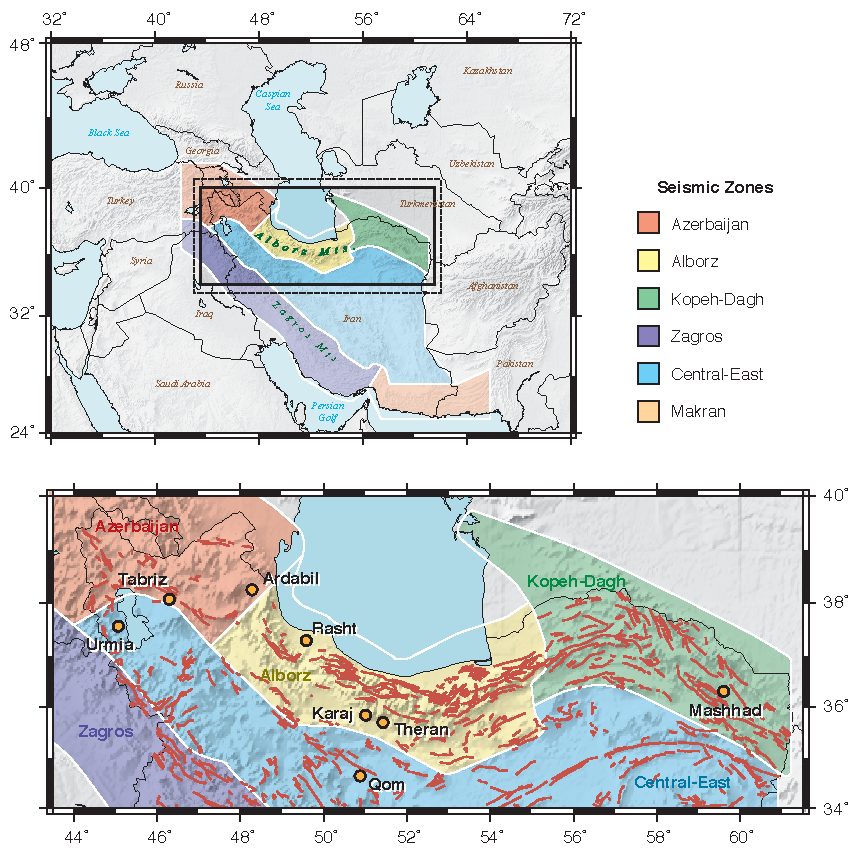
\includegraphics[width=0.9\textwidth]{figures/pdf/figure-01}
	\caption{Region of interest and Iranian seismic zones. At the top, the map of Iran and surrounding countries with shaded relief in the background and the Iranian seismic zones \citep[after][]{Karimiparidari2013} and region of interest in the foreground. The dashed box indicates the complete region of interest and the thicker line box indicates the effective area for which seismic hazard is estimated. The effective region of interest is shown in greater detail at the bottom. Details include the location of the major urban centers and seismic faults in northern Iran.}
	\label{fig:iran}
\end{figure*}

\section{Region of Interest}

Seismic activity in the Iranian plateau is dominated by the tectonic contacts between the Arabian, Eurasian, and Indian plates, which confine the region laterally between the Indian and Eurasian plates, and the Arabian and eastern Asia-Minor plates to the east and west, respectively. This setting gives rise to the Zagros, Alborz, and east Iranian mountain ranges, and defines the geology of the region. Based on these conditions, Iranian seismicity is typically divided into various seismic zones, varying from as few as four to as many as twenty-three \citep[e.g.,][]{Stocklin1968, Berberian1976, Tavakoli1999}. Here, we adopt the model proposed by \citet{Karimiparidari2013}, which consists of six seismic zones: Azerbaijan, Alborz, Kopeh-Dagh, Zagros, Central-East, and Makram (Fig.~\ref{fig:iran}).

Within this context, we define our region of interest between longitudes 43.5\textdegree{}E and 61.5\textdegree{}E, and latitudes 34\textdegree{}N and 40\textdegree{}N, as shown in Fig.~\ref{fig:iran}. These limits correspond to the effective region of interest for which we will present results ins subsequent sections. Our calculations, however, included data from a slightly larger region with a 0.5\textdegree{}-perimeter as indicated in the figure. This is done to avoid the artificial decay effect that results from smoothing the seismicity along and near the edges of the region of interest. The effective region has an area of 1,703 km $\times$ 667 km, and as shown in Fig.~\ref{fig:iran}, it encloses the northern part of Iran with most of the Azerbaijan seismic zone, the complete zones of Alborz and Kopeh-Dagh, and the northernmost portions of the Zagros and Central-East seismic zones.

At the northeast of Iran, the seismic zone of Azerbaijan is strongly controlled by the north Tabriz fault (NTF) system. This system is a complex northwest-trending structure with a predominant right-lateral, str\-ike-slip faulting mechanism \citep{Berberian1999}. Historical accounts document the occurrence of earthquakes in this area as far back as to the 9th century, with events in the years 858 ($M$ 6.0), 1042 ($M$ 7.3), 1273 ($M$ 6.5), and 1304 ($M$ 6.7) \citep{Berberian1999}. In the 18th century, in particular, the NTF ruptured three times in a span period of 65 years, which included the $M$ 7.3 1721 Shelbi earthquake in the southeastern section, the $M$ 7.4 1780 Tabriz earthquake in the northwestern section, and the $M$ 6.3 1786 Marand-Mishu on the Mishu reverse fault and the Sufian segment of the NTF. According to \citet{Jones1834}, the Shelbi and Tabriz earthquakes had surface ruptures of more than 35 and 42 km, respectively; and the latter presented vertical separations of about 2 to 4 m. Other notable events include the $M$ 5.5 1807 Tasuj and the $M$ 6.7 1879 South Bozqush earthquakes. More recently, the NTF system produced the $M_w$ 6.1 1997 Ardabil and $M_w$ 6.4 2012 Tabriz earthquakes, which caused extensive damage to the region and took the lives of more than 1500 people \citep{USGS_ardabil,USGS_tabriz}.

Transitioning from the Azerbaijan to the Alborz seismic zone, the next fault system runs along the Rocks of the Talesh mountains, to the northwest of the Alborz Mountains. Faults in this area have ruptured recently, including an $M_s$ 6.0 low-angle thrust earthquake in 1978 \citep{Berberian1999} and the $M_w$ 7.4 1990 Manjil-Rudbar earthquake, which caused numerous deaths and significant damage to the region in the south Caspian depression \citep{USGS_manjil}. At the central area of the Alborz seismic zone, near Tehran, the region is characterized by active reverse faults in the North Tehran Thrust (NTT) system. These faults are parallel to the northwest-trending structural gain of the Alborz Mountains belt, and include the south-dipping partially blind faults of Davudieh, Shian, and Bagh-E Feyz. According to \citet{Ambraseys2005}, both Tehran and the ancient city of Rey have been devastated in multiple occasions due to severe earthquakes in this area. Historical accounts document the occurrence of multiple $M>7$ earthquakes in 743, 958, 1177, 1655, and 1830. The 1830 earthquake, in particular, ruptured the central segments of the NTT, adjacent to the Mosha fault.

To the east, the Kopeh-Dagh fault system is the predominant faulting system in the seismic zone of the same name. This system consists of several partly overlapping segments parallel to a NW--SE oriented structure of step-overs characterized by short south-dipping thrust faults striking E--W \citep{Berberian2001}, which exhibits active tectonic displacements along more than 500 km \citep{Trifonov1978}. This system is responsible for the $M_s$ 7.2 earthquake that stroke Ashgabat, the capital city of Turkmenistan and destroyed more than 30 villages in Iran in 1948. Historically, the Kopeh-Dagh seismic zone is also responsible for multiple earthquakes at boundary between the Neyshabur and Binalud reverse faults between 1209 and 1405 \citep{Berberian1999}, and an estimated $M_s$ 7.1 earthquake in 10 B.C., roughly 30 kilometers from the border of Iran \citep{Berberian2001}.

% *********************************************************************************************************************
% *********************************************************************************************************************

% Naeem's original Text
% ---------------------

% With respect to different seismicity rates of the regions \citep{Nemati2015}, as well as the completeness of the seismic catalog \citep{Zare2014} , the study region is divided into three tectonic seismic zones. Each of these zones is characterized by its respective seismicity parameters values, including b-value and maximum magnitude ($M{_{max}}$). Part of Central Iran and Zagros regions are inside of the study region. We also calculated the seismicity parameters in these regions. Fig.~\ref{fig:Iran} shows the study region and different seismotectonic classification.

% \begin{figure*}[!ht] 
% \centering
% 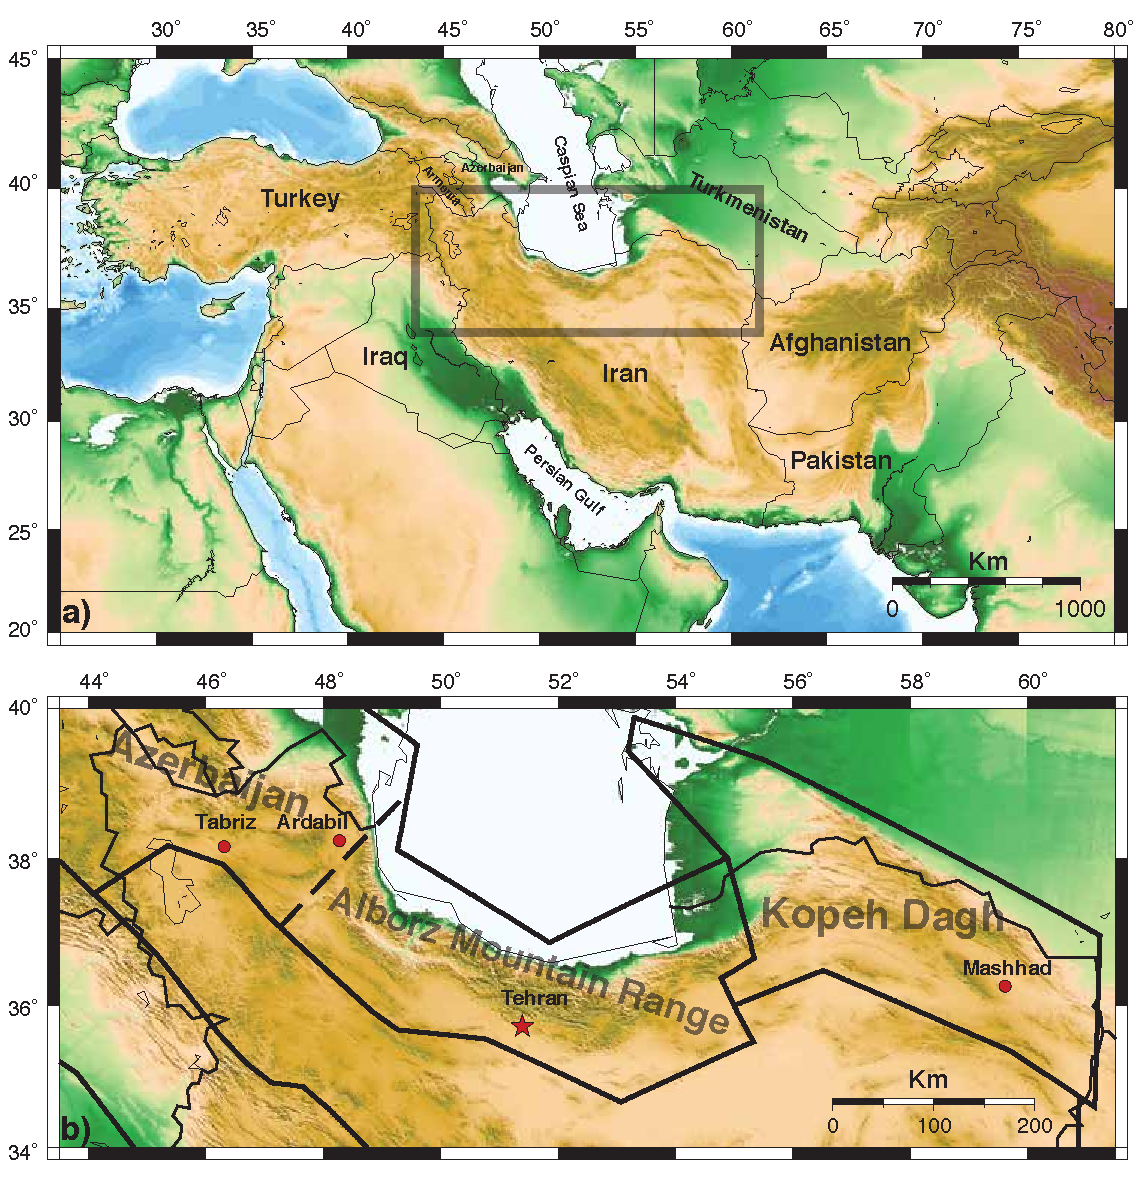
\includegraphics[scale=0.7]{figures/pdf/Figure1.pdf} 
% \caption{ a) Map of Iran and surrounding countries. The study area is presented in gray box. b) The study area containing seismotectonic provinces after \citet{Mirzaei1998}, and location of big cities. Dashed line is the subdivision that is proposed by \citet{Karimiparidari2013}. }
 
% \label{fig:Iran}
% \end{figure*}

% \subsection{Tectonic Regions and Seismic Faults}

% \subsubsection{Alborz Mountain Range (Alborz)}
% Tehran region has active reverse faults, which are parallel to the northwest-trending structural gain of the Alborz Mountains belt. Here a series of historical earthquakes occurred within a time period of more than 1100 years. Four earthquakes with magnitude more than 7 devastated the Tehran region in four centuries period, from 743 to 1177, but in the last 800 years, only one earthquake at 1830 has struck this region. At least three damaging earthquakes in 958 (western segments), 1655 (eastern segments), and 1830 (central segments), ruptured adjacent segments of the Mosha fault, located in northern Tehran.
% The North Tehran Thrust (NTT) adds more complexity due to the presence of south-dipping reverse faults, which are in part blind, such as the Davudieh, Shian, and Bagh-E Feyz.
% The northwest continuation of the Alborz Mountains, known as the Rocks of the Talesh Mountains, have been thrust northeastward and eastward over rocks of the south Caspian depression. An earthquake with Ms 6.0 in 1978 led to a focal mechanism consistent with a low-angle thrust \citep{Berberian1999}. Recently, the 1990 $M_w$ 7.4 Manjil-Rudbar earthquake caused extensive loss of life and significant damage \citep{USGS_manjil}. Based on existing documents, Tehran city and ancient Rey city have been destroyed completely several times by severe earthquakes with magnitudes greater than 7 \citep{Ambraseys2005}. \\

% \subsubsection{Azerbaijan}
% There were three earthquakes from 1721-86 that ruptured the North Tabriz Fault system from southeast to northwest. The Tabriz region is in the Araxes structural block of northwestern Iran, southwest of the continuation of the western Alborz Mountains towards the Caucasus. The North Tabriz Fault (NTF) is a complex northwest-trending structure, which contains evidence observed on aerial photographs, and vertical displacement with the north side up, of right-lateral strike-slip displacement \citep{Berberian1999}.
% The NTF system and nearby reverse faults ruptured from southeast to northwest in three earthquakes over 65 years: the Shebli earthquake with magnitude 7.3 in 1721 on the southeastern NTF with a surface rupture more than 35 km long, reported by \citet{Jones1834} the Tabriz earthquake with magnitude 7.4 in 1780 on the northwestern NTF, with a surface rupture more than 42 km long and vertical separation of 2 to 4 $m$; and the Marand-Mishu earthquake with magnitude of 6.3 in 1786 on the Mishu reverse fault and the Sufian segment of the NTF. Another earthquake with  magnitude 5.5 struck the Tasuj reverse fault farther west in 1807 and an earthquake of M 6.7 took place along the South Bozqush reverse fault farther southeast in 1879. Prior to the 1721-86 earthquake sequence, Tabriz was shaken by earthquakes in 858 (M 6.0), 1042 (M 7.3), 1273 (M ~ 6.5), and 1304 (M 6.7)\citep{Berberian1999}. Most recently, earthquakes with $M_w$ 6.1 in 1997 and $M_w$ 6.4 in 2012 occurred in Ardabil and Tabriz, respectively. These earthquakes caused around 1500 casualties and extensive damage \citep{USGS_ardabil,USGS_tabriz}.\\


% \subsubsection{Kopeh Dagh}
% The main Kopeh-Dagh fault system has experienced some historic earthquakes. Ashgabat, the capital city of Turkmenistan, was destroyed by an earthquake of Ms 7.2 in 1948 and destroyed more than 30 villages in Iran. This was the strongest earthquake to strike this region since at least 1455.
% The main Kopeh-Dagh fault consists of several partly overlapping segments parallel to the overall $NW - SE$ structure with step-overs. The regions of overlap are characterized by shorter south-dipping thrust faults striking about $E - W$ \citep{Berberian2001}. \citet{Trifonov1978} reported active displacement along the main Kopeh-Dagh fault for more than 500 km. 
% Massive destruction of the capital city of Mithradatkert is attributed to the 10 BC event Ms 7.1, roughly 30 kilometers from the border of Iran (Nesa mound) \citep{Berberian2001}.
% The Neyshabur sequence of four earthquakes between 1209 and 1405 respected the segment boundary between the Neyshabur and Binalud reverse fault system \citep{Berberian1999}.
% Historical records show that in 1209, the district of Neyshabur from Neyshabur city in the west to Daneh village in the east was totally destroyed \citep{Berberian1999}.\\



% \subsection{Historical  and Instrumental Seismicity}
% Uniform earthquake catalog is the most important factor in seismic hazard analysis of a region.  Different studies have been conducted in order to prepare a uniform catalog for Iranian Earthquake. Historical event interpretation and different magnitude conversion relationships are some of the factors which make all these catalogs different. Among different sources \citet{Ambraseys2005}, \citet{Berberian1994}, and \citet{moinfar1994} are some of the main sources for Iranian earthquake catalog. These catalogs contain historical and instrumental earthquakes that have been reported in literature and national and international networks. According to \citet{Ambraseys2005}, there are some scattered indication of earthquake effects  back to third millinuim BC. However, adequate documentary coverage of individual events begins from seventh century A.D. \citet{Mirzaei1997} provided a comprehensive list of studies that have been done in compilation a uniform catalog for Iranian earthquakes in order to prepare a uniform catalog of earthquake (all earthquakes are converted to surface wave magnitude Ms) for seismic hazard assessment in Iran. The catalog is covering the period of 4th century B.C. through 1994. The instrumental data is achievable from three national agencies including IIEES, International Institute of Earthquake Engineering and Seismology; IRSC, The Iranian seismological center, University of Tehran; and BHRC, Building and Housing Research Center (Iran Strong Motion Network) (For more information about these networks see \citet{Karimiparidari2013}).
% Many most of attenuation relationship use  moment magnitude $M_w$ as an input for the equation \citep{Douglas2011}. Moment magnitude is not suffering from saturation and has physical meaning \citep{Kanamori1977}. Due to mentioned reasons Mw has become a most appropriate magnitude scale in recent studies. 
%  \citet{Karimiparidari2013}compiled a uniform earthquake catalog for Iran and adjacent areas, using international and national databanks until April 2010.  They developed relationships between moment magnitude and other magnitude based on orthogonal regression.  They removed the dependent events (aftershocks and foreshocks) using the procedure by \citet{Gardner1974}. The catalog of events with magnitude equal and above Mw 5.5 is provided. 
% \citet{Shahvar2013} presented a unified and homogeneous catalog for the Iranian plateau $(M_w >= 4)$, created by merging data from two local catalogs and seven international agencies for 1900-2011 period. They used orthogonal regression method \citep{Castellaro2006} to derive magnitude conversion relation. By removing foreshocks and aftershocks according to the procedure detailed in Uhrhammer(1986), they also provided declustered version of the catalog.

% The recent unified catalog for Middle East region is published as a part of Global Earth Model (GEM) and the Earthquake Model of the Middle East (EMME) project by \citet{Zare2014}. They used all historical (pre-1900), early and modern instrumental events up to 2006. The catalog contains data from Alborz-Azerbaijan, Afghanistan-Pakistan, Saudi Arabia, Caucasus, Central Iran, Kopeh-Dagh, Makran, Zagros, and part of Turkey. The magnitude of all events are converted to Mw through relationships which is derived at previous studies or newly derived at the study relationships. They declustered data through different methods including \citet{Gardner1974}, Uhrhammer(1986), \citet{Reasenberg1985}, and Gruenthal. \citet{Zare2014} provided the catalog completeness for different magnitude range using  the cumulative frequency-magnitude distribution of  \citet{Gutenberg1944} and \citet{richter1958}, and frequency magnitude distributaion of ZMAP \citep{Wiemer2001} software. The methods confirms the results of each other. 

% In this study we consider earthquakes with Mw equal and greater than 3. Earthquakes with magnitude 3 are not considered as a structural threat, however, the epicenter of earthquakes with magnitude $M_w 3$ are a  susceptible location for future bigger earthquakes.  According to our preliminary data processing based on IIEES data, Iranian catalog for earthquake with magnitude greater and equal 3, is complete from 2005. In order to make sure about the completeness of the catalog, we use IIEES data from 2000. We used the EMME project data provided by \citet{Zare2014} up to 2000. Fig.~\ref{fig:historical} represents the historical data (pre 1900) in the study region. 

% \subsubsection{Magnitude Conversion}

% The catalog of recorded earthquake from 2000-2015 which is downloaded from IIEES is reported the earthquake based on different magnitude scale. We converted the $M_L$, $M_s$, and $mb$ magnitudes through conversion relationships which is defined in \citet{Zare2014}. There also some of data which is recorded in $M_D$ (Duration magnitude). These data are reported by International Seismological Centre (ISC).  \citet{Deniz2010}, developed a set of empirical equations to convert earthquake magnitudes in $mb$, $M_D$, $M_L$ and $M_s$ scales to the $M_w$ scales using orthogonal regression procedure. They used data of earthquake that occurred in Turkey from different data centers including ISC. In this study we use the conversion equation of \citet{Deniz2010} to convert the Md to Mw. Although they defined the equation based on $M_w>=4.5$, we extrapolate the equation for lower magnitude. We believe having those earthquakes, even with small error  in magnitude is important for estimating an accurate "a" value  in Gutenberge-Richter equation.

% \begin{figure*}[!ht] 

% \centering
% \includegraphics[scale=0.4]{figures/pdf/Figure2.pdf} 
% \caption{Historical earthquakes of Iran (pre 1900). Different colors represent different year of occurrences and size of circles are proportional to the earthquake magnitude. }
% \label{fig:historical}
% \end{figure*}


% \subsubsection{Declustering}

% It is generally assumed that the seismicity of each tectonic seismic source follows a Poissonian occurrence process. Therefore, in order to accomplish this, we declustered the earthquake catalog. In compiling the catalog of events, foreshocks and aftershocks were removed using a declustering methodology \citep{Gardner1974}. For north Iran (lon: 42-62.5, lat: 33-41), from 7478 earthquake event we removed 605 Foreshocks and 2917 aftershocks.
% Whole data that we used for seismicity parameters of Zagros and Central Iran tectonic seismic regions are not included in these numbers. Fig.~\ref{fig:instrumental} shows the epicenter of declustered instrumental  earthquakes.


% \begin{figure*}[!ht] 

% \centering
% 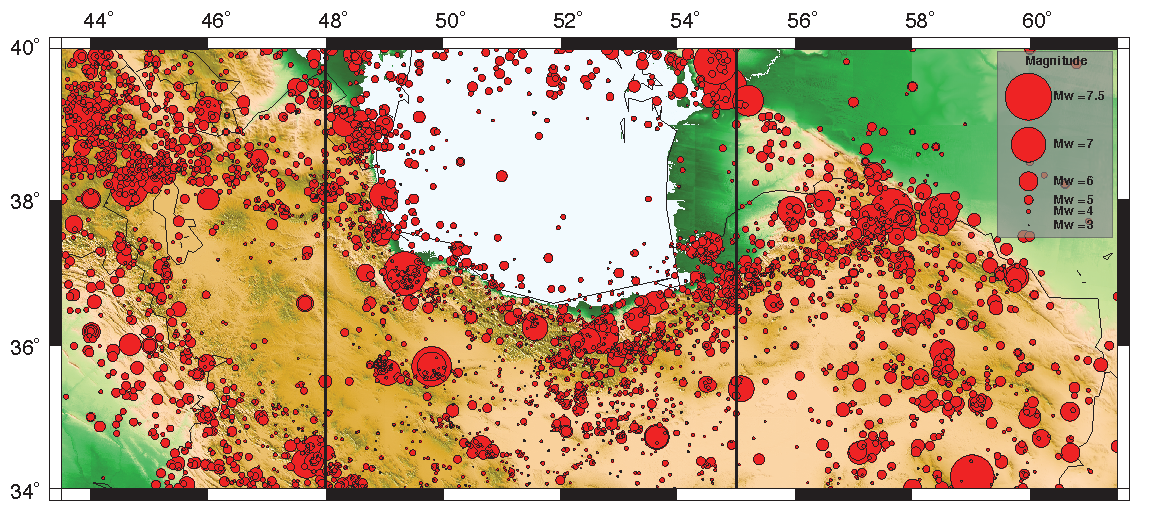
\includegraphics[scale=0.25]{figures/pdf/Figure3.pdf} 
% \caption{Declustered instrumental seismicity map (after 1900) of Northern Iran. The study areas are separated at longitude of 48$^{\circ}$ and 55$^{\circ}$ . } 
% \label{fig:instrumental}
% \end{figure*}


% \subsection{Divisions}

% As we discussed earlier (see the Introduction section), classifying the tectonic seismic regions has been a controversial debate. In this study we consider two seismic tectonic models. First model is according to \citet{Mirzaei1998} and \citet{Karimiparidari2013} classification, which includes Azerbaijan, Alborz, Kopek Dagh, and part of Central Iran, and Zagros, the second model is a uniform model for the whole north Iran.  



\begin{figure*}[t] 
	\centering
	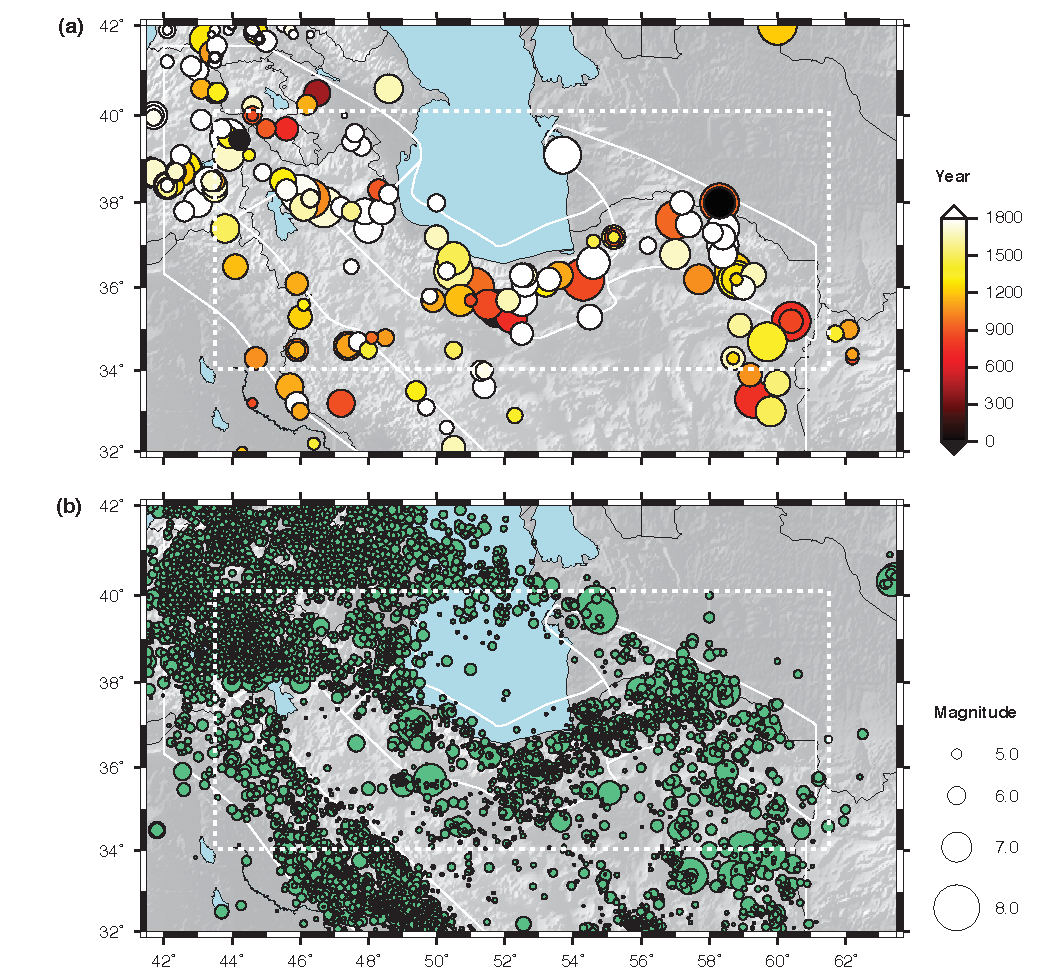
\includegraphics[width=0.9\textwidth]{figures/pdf/figure-03}
	\caption{Location of events considered in the compiled seismic catalog. (a) Historical seismicity prior to 1900 for $M_w \geq 4$ \citep[after][]{Zare2014}. (b) Instrumental seismicity up until December 2015 for $M_w \geq 3$ (IIEES) and $M_w \geq 4$ \citep[after][]{Zare2014}. Size of symbols is proportional to the magnitude of the events. In the case of the historical seismicity catalog, the color fill indicates the year of the event. The borderlines of the seismic zones shown in Fig.~\ref{fig:iran} are shown in the background in white, along with the light gray shaded relief.}
	\label{fig:catalog}
\end{figure*}

\section{Seismic Catalog}

A fundamental step in regional seismic hazard analysis is the compilation of a reliable seismic catalog that includes both historically documented and instrumentally recorded earthquakes. Nowadays, instrumental datasets are easily accessible through international, regional, and local agencies. Historical data, on the other hand, lends itself to subjective interpretation. Notable previous efforts to compose uniform earthquake catalogs for Iran include but are not limited to \citet{Ambraseys_1982_Book}, \citet{moinfar1994}, and \citet{Berberian_1995_Tech}. These studies, however, differ from each other in their use of magnitude scales or magnitude conversion rules, and the extent to which they accept historical accounts as valid data. 

According to \citet{Ambraseys_1982_Book}, there is evidence of earthquakes as far back as the third millennium B.C., yet some of those accounts are difficult to interpret. \citet{Mirzaei1997} compiled a catalog with historical events dating back to the 4th century B.C.~and instrumental earthquakes through 1994 in which a comprehensive list of studies was considered and magnitudes uniformly converted to surface wave magnitude ($M_s$). Most ground motion prediction equations employed today in seismic hazard, however, use moment magnitude ($M_w$) instead. 

Recent catalogs such as that by \citet{Karimiparidari2013}, \citet{Shahvar2013}, and \citet{Zare2014} are all compiled using magnitudes converted to $M_w$. \citet{Karimiparidari2013}, for instance, compiled a catalog for Iran and adjacent areas using international and national datasets including events up until April, 2010, with $M_w > 5$. They developed relationships between moment magnitude and other magnitude scales and removed foreshocks and aftershocks using the procedure by \citet{Gardner1974}. \citet{Shahvar2013} built a catalog for the Iranian plateau for events with $M_w \geq 4$ merging data from two local and seven international datasets for the 1900--2011 period. They used the orthogonal regression method by \citet{Castellaro2006} to derive magnitude conversions and removed foreshocks and aftershocks according to the procedure by \citet{Uhrhammer_1986_EN}. In addition, \citet{Shahvar2013} provided a declustered version of the catalog. 

In this study we adopt the catalog compiled for the Middle East by \citet{Zare2014} and complement it for our particular region of interest. This catalog is particularly relevant because it is published as part of the current effort by the Global Earthquake Model (GEM) partnership and the Earthquake Model of the Middle East (EMME) project. It combines over 28 thousand records from 26 datasets with both historical and instrumental seismicity. Instrumental datasets included information from international, regional, and local agencies and networks, such as the U.S.~Geological Survey's National Earthquake Information Center (NEIC), the International Seismological Center (ISC) bulletins, the International Institute of Earthquake Engineering and Seismology (IIEES), the Iranian Seismological Center (IRSC) at the University of Tehran, and the Iranian Strong Motion Network operated by the Building and Housing Research Center (BHRC), among others. Historical data included the datasets prepared over the years by \citet{Ambraseys_1982_Book}, \citet{Ambraseys_2005_Book}, and \citet{Ambraseys_2009_Book}.

For the particular case of our region of interest, the catalog prepared by \citet{Zare2014} included events $M_w \geq 4$ between 550 B.C.~and 2006. We took information from the catalog up to December 1999, and complemented it by adding newer and more complete data from IIEES for events $M \geq 3$ between January 2000 and December 2015. While we recognize that earthquakes in the range $3 \leq M_w \leq 4$ are unlikely to cause structural damage, we include them as a means to feed the model with information about epicentral locations with potential for future larger magnitude earthquakes. By contrast, a recent seismic hazard analysis done for Iran by \citet{Khodaverdian_2016_BSSA} used a similar for events $M_w \geq 4$ catalog but only included data up until 2011, which excluded the 2012 $M_w$ 6.4 Tabriz earthquake that severely damaged the northeast part of the country.

In terms of magnitude scale, the events in \citet{Zare2014} were converted from $M_L$, $M_s$ and $m_b$ scales to $M_w$ using relationships derived by the authors and by \citet{Escordilis_2006_JS}. For consistency, we used the same conversion relationships for the portion of the catalog obtained from IIEES for $M \geq 3$ earthquakes between 2000 and 2015. The dataset from IIEES also contained events reported by ISC on a duration magnitude ($M_D$) scale. In these cases we used the empirical relationship introduced by \citet{Deniz2010} to convert $M_D$ to $M_w$. Although this relationship was derived based on a dataset for $M_w \geq 4.5$ events, we extrapolated the equation for lower magnitudes and found the results to adjust well with the general trend. 

Selection and declustering was also done in consistence with the original catalog, using the methods by \citet{Gardner1974}, \citet{Reasenberg1985} and \citet{Uhrhammer_1986_EN}. We obtained the declustered version of \citet{Zare2014}, selected 7,478 earthquakes within our region of interest, and removed 605 foreshocks and 2,917 aftershocks, leaving only those events in agreement with a Poissonian model. The same procedure was used for the added events between 2000 and 2015. These steps altogether allowed us to preserve compatibility with the original catalog while also including the most recent events. The final set of events compiled for this study is shown in Fig.~\ref{fig:catalog}.


% *********************************************************************************************************************
% *********************************************************************************************************************

% ***** In addition, \citet{Zare2014} provided the catalog completeness for different magnitude ranges using the cumulative frequency-magnitude distribution of \citet{Gutenberg1944} and \citet{richter1958}, and the frequency magnitude distribution obtained using ZMAP \citep{Wiemer2001}, and found these methods to yield consistent results. 

% **** Our analysis of this dataset indicated that the catalog satisfies completeness from 2005 onward. 

% *********************************************************************************************************************
% *********************************************************************************************************************

% \citet{Zare2014} uses both historical data prior to 1900 and instrumental data up until 2006, including events from Afghanistan, Pakis\-tan, Saudi Arabia, the Caucasus and parts of Turkey, in addition to the Alborz-Azerbaijan, Zagros, central Iran, Kopeh-Dagh and Makran seismic zones. 

% All events in this catalog are converted to $M_w$ using relationships derived by the authors and by \citet{Escordilis_2006_JS}; and declustered using various methods \citep{Gardner1974, Reasenberg1985, Uhrhammer_1986_EN}. 

% This catalog is particularly relevant because it is published as part of the current effort by the Global Earthquake Model (GEM) partnership and the Earthquake Model of the Middle East (EMME) project.

% In this study we adopt the catalog compiled by \citet{Zare2014} for both historical and instrumental earthquakes. This catalog includes events of magnitude $M_w \geq 4$ from 550 A.d.~to December 1999. 

% We complemented it with events $M \geq 3$ occurred between January 2000 and December 2015 obtained from the IIEES database. 

% The result of our compilation is shown in Fig.~\ref{fig:catalog}, which includes maps for historical and instrumental seismicity. 
% The following sections provide additional details about magnitude conversion and de\-clustering of the events in our combined catalog.

% The portion of the catalog obtained from IIEES for $M \geq 3$ earthquakes between 2000 and 2015 contained event reports that use different magnitude scales. We converted all events with magnitudes in $M_L$, $M_s$, and $mb$ scales to $M_w$ using the same conversion relationships used by \citet{Zare2014}, which allowed us to preserve compatibility with the historical and instrumental seismicity catalog adopted from the same work of \citet{Zare2014}. 

% Last but not least important, we declustered the catalog prior to using it in the assessment of seismic hazard for the region of interest. This entailed the removal of foreshocks and aftershocks from the catalog to adjust the dataset to include only those events in agreement with a Poissonian model, which is a well-accepted model for seismic sources. Out of the original 7,478 earthquakes in the assembled catalog for the seismic regions of Azerbaijan, Alborz and Kopeh-Dagh, we removed 605 foreshocks and 2,917 aftershocks. The resulting final set of events in the catalog compiled for this study is shown in Fig.~\ref{fig:catalog}, which includes maps for both historical and instrumental seismicity.

% *********************************************************************************************************************
% *********************************************************************************************************************

% Naeem's original Text
% ---------------------

% \subsection{Historical  and Instrumental Seismicity}

% Uniform earthquake catalog is the most important factor in seismic hazard analysis of a region.  Different studies have been conducted in order to prepare a uniform catalog for Iranian Earthquake. Historical event interpretation and different magnitude conversion relationships are some of the factors which make all these catalogs different. Among different sources \citet{Ambraseys2005}, \citet{Berberian1994}, and \citet{moinfar1994} are some of the main sources for Iranian earthquake catalog. These catalogs contain historical and instrumental earthquakes that have been reported in literature and national and international networks. According to \citet{Ambraseys2005}, there are some scattered indication of earthquake effects  back to third millinuim BC. However, adequate documentary coverage of individual events begins from seventh century A.D. \citet{Mirzaei1997} provided a comprehensive list of studies that have been done in compilation a uniform catalog for Iranian earthquakes in order to prepare a uniform catalog of earthquake (all earthquakes are converted to surface wave magnitude Ms) for seismic hazard assessment in Iran. The catalog is covering the period of 4th century B.C. through 1994. The instrumental data is achievable from three national agencies including IIEES, International Institute of Earthquake Engineering and Seismology; IRSC, The Iranian seismological center, University of Tehran; and BHRC, Building and Housing Research Center (Iran Strong Motion Network) (For more information about these networks see \citet{Karimiparidari2013}).

% Many most of attenuation relationship use  moment magnitude $M_w$ as an input for the equation \citep{Douglas2011}. Moment magnitude is not suffering from saturation and has physical meaning \citep{Kanamori1977}. Due to mentioned reasons Mw has become a most appropriate magnitude scale in recent studies. 

%  \citet{Karimiparidari2013}compiled a uniform earthquake catalog for Iran and adjacent areas, using international and national databanks until April 2010.  They developed relationships between moment magnitude and other magnitude based on orthogonal regression.  They removed the dependent events (aftershocks and foreshocks) using the procedure by \citet{Gardner1974}. The catalog of events with magnitude equal and above Mw 5.5 is provided. 
% \citet{Shahvar2013} presented a unified and homogeneous catalog for the Iranian plateau $(M_w >= 4)$, created by merging data from two local catalogs and seven international agencies for 1900-2011 period. They used orthogonal regression method \citep{Castellaro2006} to derive magnitude conversion relation. By removing foreshocks and aftershocks according to the procedure detailed in Uhrhammer(1986), they also provided declustered version of the catalog.

% The recent unified catalog for Middle East region is published as a part of Global Earth Model (GEM) and the Earthquake Model of the Middle East (EMME) project by \citet{Zare2014}. They used all historical (pre-1900), early and modern instrumental events up to 2006. The catalog contains data from Alborz-Azerbaijan, Afghanistan-Pakistan, Saudi Arabia, Caucasus, Central Iran, Kopeh-Dagh, Makran, Zagros, and part of Turkey. The magnitude of all events are converted to Mw through relationships which is derived at previous studies or newly derived at the study relationships. They declustered data through different methods including \citet{Gardner1974}, Uhrhammer(1986), \citet{Reasenberg1985}, and Gruenthal. \citet{Zare2014} provided the catalog completeness for different magnitude range using  the cumulative frequency-magnitude distribution of  \citet{Gutenberg1944} and \citet{richter1958}, and frequency magnitude distributaion of ZMAP \citep{Wiemer2001} software. The methods confirms the results of each other. 

% In this study we consider earthquakes with Mw equal and greater than 3. Earthquakes with magnitude 3 are not considered as a structural threat, however, the epicenter of earthquakes with magnitude $M_w 3$ are a  susceptible location for future bigger earthquakes.  According to our preliminary data processing based on IIEES data, Iranian catalog for earthquake with magnitude greater and equal 3, is complete from 2005. In order to make sure about the completeness of the catalog, we use IIEES data from 2000. We used the EMME project data provided by \citet{Zare2014} up to 2000. Fig.~\ref{fig:historical} represents the historical data (pre 1900) in the study region. 

% \subsubsection{Magnitude Conversion}

% The catalog of recorded earthquake from 2000-2015 which is downloaded from IIEES is reported the earthquake based on different magnitude scale. We converted the $M_L$, $M_s$, and $mb$ magnitudes through conversion relationships which is defined in \citet{Zare2014}. There also some of data which is recorded in $M_D$ (Duration magnitude). These data are reported by International Seismological Centre (ISC).  \citet{Deniz2010}, developed a set of empirical equations to convert earthquake magnitudes in $mb$, $M_D$, $M_L$ and $M_s$ scales to the $M_w$ scales using orthogonal regression procedure. They used data of earthquake that occurred in Turkey from different data centers including ISC. In this study we use the conversion equation of \citet{Deniz2010} to convert the Md to Mw. Although they defined the equation based on $M_w>=4.5$, we extrapolate the equation for lower magnitude. We believe having those earthquakes, even with small error  in magnitude is important for estimating an accurate "a" value  in Gutenberge-Richter equation.

% \begin{figure*}[!ht] 

% \centering
% \includegraphics[scale=0.4]{figures/pdf/Figure2.pdf} 
% \caption{Historical earthquakes of Iran (pre 1900). Different colors represent different year of occurrences and size of circles are proportional to the earthquake magnitude. }
% \label{fig:historical}
% \end{figure*}

% \subsubsection{Declustering}

% It is generally assumed that the seismicity of each tectonic seismic source follows a Poissonian occurrence process. Therefore, in order to accomplish this, we declustered the earthquake catalog. In compiling the catalog of events, foreshocks and aftershocks were removed using a declustering methodology \citep{Gardner1974}. For north Iran (lon: 42-62.5, lat: 33-41), from 7478 earthquake event we removed 605 Foreshocks and 2917 aftershocks.
% Whole data that we used for seismicity parameters of Zagros and Central Iran tectonic seismic regions are not included in these numbers. Fig.~\ref{fig:instrumental} shows the epicenter of declustered instrumental  earthquakes.

% \begin{figure*}[!ht] 

% \centering
% 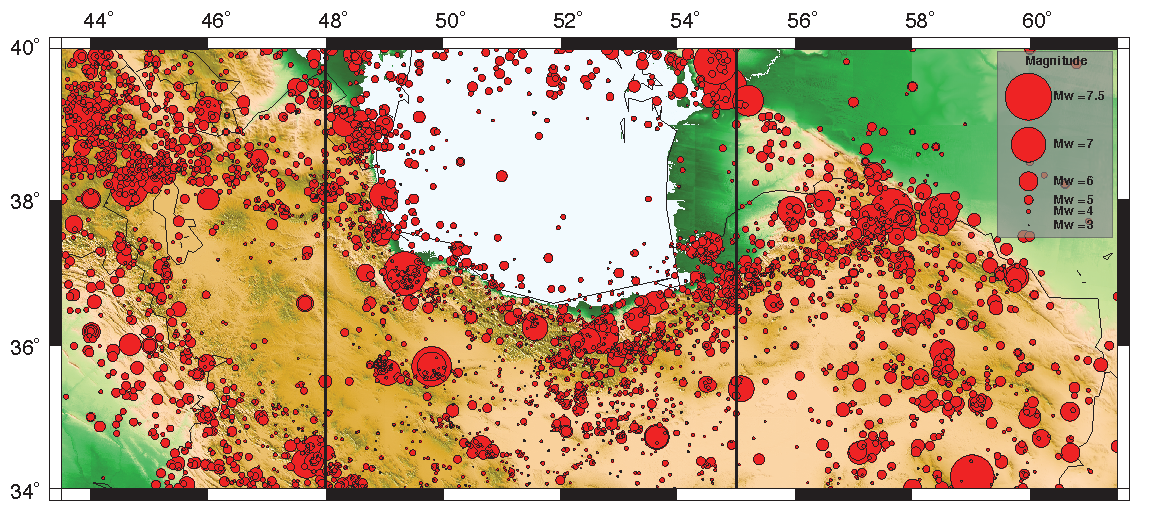
\includegraphics[scale=0.25]{figures/pdf/Figure3.pdf} 
% \caption{Declustered instrumental seismicity map (after 1900) of Northern Iran. The study areas are separated at longitude of 48$^{\circ}$ and 55$^{\circ}$ . } 
% \label{fig:instrumental}
% \end{figure*}

% \subsection{Divisions}

% As we discussed earlier (see the Introduction section), classifying the tectonic seismic regions has been a controversial debate. In this study we consider two seismic tectonic models. First model is according to \citet{Mirzaei1998} and \citet{Karimiparidari2013} classification, which includes Azerbaijan, Alborz, Kopek Dagh, and part of Central Iran, and Zagros, the second model is a uniform model for the whole north Iran.  



\section{Seismic Hazard Approach}

There have been multiple assessments of seismic hazard for Iran. A brief report on the most recent review done to define the hazard zoning map of Iran included in the Iranian seismic code \citep{BHRC2014} can be found in \citet{Moinfar_2012_WCEE}. Other previous efforts include, for instance, the work of \citet{Tavakoli1999}, who presented iso-acceleration contour lines and seismic hazard zonation for Iran based on known major fault-lines and area-source models; the results obtained by \citet{Ghodrati2003}, who presented a refined hazard assessment for the metropolitan area of Tehran using a logic tree approach to combine results from three attenuation relationships; and the recent study by \citet{Khodaverdian_2016_BSSA}, who used a smoothed seismicity approach to estimate spatially variable seismicity parameters for the whole country.

Once a seismic catalog has been defined, the second most important step is precisely the definition of the seismicity parameters $a$ and $b$ used in the Gutenberg-Richter recurrence relation 
% 
\begin{equation}
	\log_{10} N = a - b M \, ,
\end{equation}
% 
\noindent
where $N$ is the number of earthquakes with magnitude greater than or equal to $M$, $a$ accounts for the number of earthquakes that occur within a given region, and $b$ is a measure of the occurrence of earthquakes relative to magnitude \citep{Gutenberg1944}. These parameters can be assumed constant within a region or spatially variable depending on the approach used. 

In this study we use the smoothed seismicity method introduced by \citet{Frankel1995}. This method has been used successfully in different regions around the world including Alaska, California, Hawaii, Italy, \myrevision{and} Turkey \citep[e.g.,][]{Cao1996, Klein2001, Akinci2004, Kalkan2009, Moschetti2014}. In it, the $b$-value is commonly assumed constant within a given seismic zone of ``homogeneous'' seismogenic characteristics, whereas $a$ is varied spatially according to the cataloged occurrence of earthquakes within and around the region. The spatial variation of $a$ is defined based on dividing the region of interest into regular-size grid cells. The parameter $a$ is determined based on the number of events $n_i$ within each cell $i$ of magnitude greater than a reference value $M_{\mathrm{ref}}$, and discretized in different magnitude ranges (or bins). The number of earthquakes within each cell is then smoothed spatially taking into account the values of neighboring cells using a Gaussian function. In essence, the smoothed seismicity approach addresses the aleatoric uncertainty of future earthquake locations by using a weighted contribution of the background regional seismicity, and thus eliminates the need for knowledge about specific fault locations.

In this study we discretize the region of interest into a regular grid with cells of size 0.1\textdegree{} $\times$ 0.1\textdegree{} (in longitude and latitude). The parameter $a$ for each cell is obtained based on the information in the seismic catalog described in the previous section. Following \citet{Frankel1995}, $n_i$ is smoothed using the normalized Gaussian function
% 
\begin{equation}
	\tilde{n}_i = \frac
		{ \sum_{j} n_{j} \exp ( \frac{ -\Delta_{ij}^{2} }{ c^2 } ) }
		{ \sum_{j} \exp ( \frac{ -\Delta_{ij}^{2} }{ c^2 } ) }
	\, ,
	\label{eq:nnorm}
\end{equation}
% 
where $\tilde{n}_i$ is the smoothed, normalized number of events in cell $i$, $\Delta_{ij}$ is the distance between the $i$-th and $j$-th cells, and $c$ is the correlation distance. The summations in Eq.~\ref{eq:nnorm} are calculated over the number of $j$ cells within a distance $3c$ from the $i$-th cell. It should be noted that in this process we convert the cumulative number of events to incremental values following \citet{Herrmann1977}. We also note that according to \citet{Frankel1995}, moderate earthquakes generally occur in areas where there have been significant numbers of events with magnitudes $M \geq 3$, thus our interest in having augmented the earthquake catalog for events above this threshold.

It is obvious from Eq.~\ref{eq:nnorm} that an important parameter in smoothing the seismicity is the correlation distance. Different values of $c$ have been used in past studies, ranging between 10 and 50 km. \citet{Frankel1995} and \citet{Boyd2008} assumed a correlation distance of 50~km, \citet{Foteva2006} used 10 and 15 km, \citet{Barani2007} used 25~km, and \citet{Khodaverdian_2016_BSSA} used 40 km. According to \citet{Mirzaei1997}, determining an appropriate value of $c$ depends on the crustal structure of the region, the distribution of stations, and the number and quality of records. We use an intermediate value of $c=30$~km. This selection is consistent with epicentral uncertainty for previous hazard zoning maps for Iran \citep[see][]{Zare2012}.

In turn, we consider the $b$-values to be constant within each seismic zone as delimited in Fig.~\ref{fig:iran}. Details about the calculation of the $b$-value for each zone are provided \myrevision{in the next section}. By contrast, in the recent work by \citet{Khodaverdian_2016_BSSA}, the authors computed spatially-variable $b$-values within large grid-cells of size 1\textdegree{} $\times$ 1\textdegree{} based on the average seismicity within a 200-km radius from each cell. While gridding $b$-values and considering the influence of neighboring large-size cells allows \myrevision{one} to draw information from the background seismicity, it is unavoidable to have the contributing areas cross over seismic zones of different characteristics, which may bias the computation of $b$-values. Admittedly, these are subjective decisions and any reasonable choice can be considered valid or within the margins of the associated epistemic uncertainty.

Last, the annual rate $\lambda$ of exceeding a reference ground motion $u_o$ is defined by
% 
\begin{align}
	\lambda & \left( u > u_o \right) = \nonumber \\
		& \sum_{k} \sum_{l} 10^{ {}^{ \left[ \log \left( \frac{ N_{k} }{ T } \right) - b \left( M_l - M_{\mathrm{ref}} \right) \right] } }
		P \left( u > u_o | D_k , M_l \right)
		\, .
	\label{eq:exceed}
\end{align}
% 
Here, the values of $\tilde{n}_i$ have been previously binned by their distance from the site of interest, $N_k$ is the total of $\tilde{n}_i$ values for cells within a certain bin distance, $T$ is the time in years used to determine $N_k$, and $k$ and $l$ are the indexes of the distance and magnitude bins, respectively. $P ( u > u_o | D_k , M_l )$ is the probability of $u$ exceeding $u_o$ given an earthquake of magnitude $M_l$ at a distance $D_k$ \citep{Frankel1995}.

It is clear from Eq.~\ref{eq:exceed} that the hazard calculations depend also on the choice of an attenuation relationship to predict the level of ground motion at a site ($u$) for any given earthquake. In the following two sections we describe how we obtained the $b$-values for the different seismic zones influencing the hazard in northern Iran and our choice of a suitable attenuation relationship (ground motion prediction equation).




\section{Seismicity Parameters}

For each of the three seismic regions, Gutenberg-Richter parameters and maximum magnitude ($M_{max}$) were calculated using Seismic Hazard Assessment code (HA3) \citep{kijko2004}. The regional maximum magnitude for each region is estimated by the \citet{Kijko1989} method, which is implemented in the HA3 package. For smoothed seismicity areas, $b-value$ is assumed constant. The $a-value$ can vary spatially and is determined by counting earthquakes above $M$ 3.0 in each grid cells.

\citet{Karimiparidari2013} applied the Maximum Curvature (MAXC) technique \citep{Wyss1999, Wiemer2000} by ZMap \citep{Wiemer2001} to calculate the level of completeness of instrumental part of the catalog.  Following the \citet{Karimiparidari2013}, we assume the catalog is complete for earthquakes with magnitude 4.5, 4.4, 4.5, 4.5, and 4.4 for Azerbaijan, Alborz,  Kopeh-Dagh, Central Iran, and Zagros tectonic seismic regions, respectively. For the uniform model we used 4.5 as a completeness magnitude. In this study we use those magnitudes of completeness as the magnitude threshold in the calculation of the seismicity parameters. We also used the seismicity parameters of \citet{Karimiparidari2013} as the priory information in HA3 code. The updated values are displayed in Table \ref{tab:b_value}.  Annual occurrence rate of the earthquake for each region is shown in Fig.~\ref{fig:annual_m}.

\begin{figure*}[t]
    \centering
    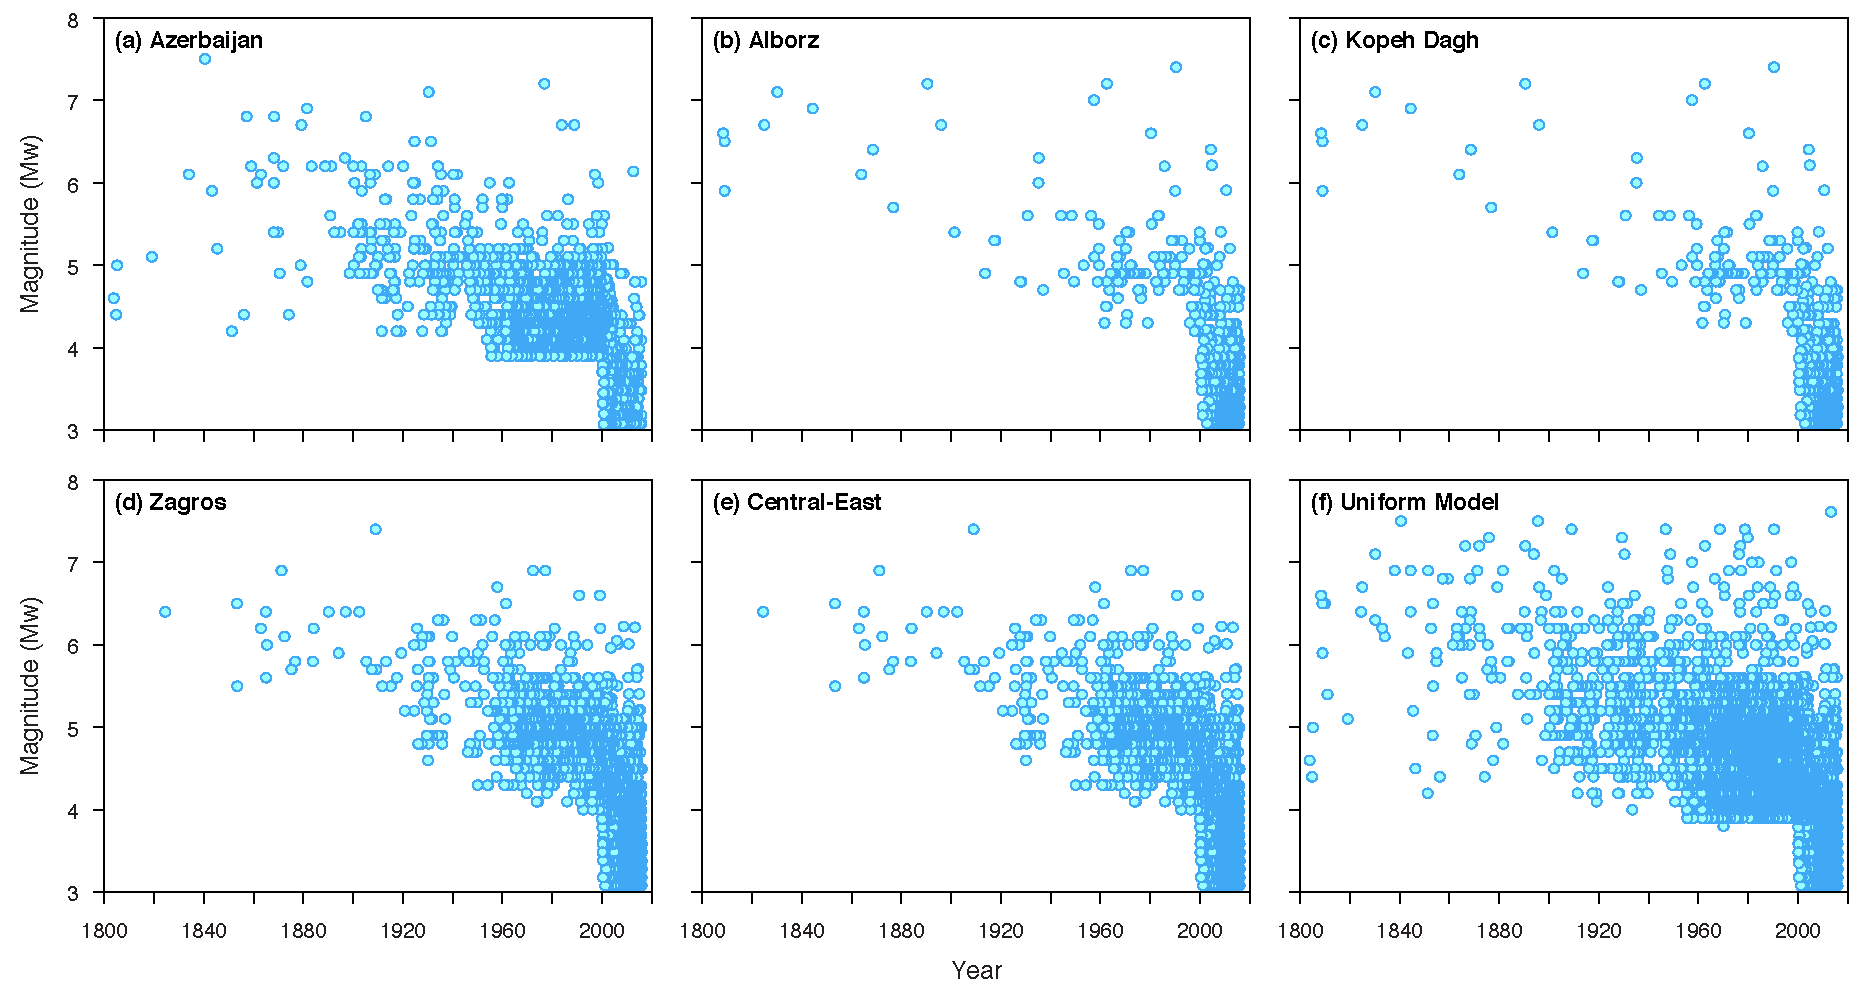
\includegraphics[width=\textwidth]{figures/pdf/figure-04} 
    \caption{Annual probability of exceedance as a function of earthquake magnitude for seismic tectonic regions of (a) Alborz, (b) Azerbaijan, (c) Central Iran, (d) Kopeh Dagh, (e) Uniform (f) Zagros. The shaded range indicates the models' $\pm 1$ standard deviation.}
    \label{fig:annual_m}
\end{figure*}

\begin{table*}[t]
    \centering
    \caption{Seismicity parameters for the tectonic seismic regions influencing seismic hazard in northern Iran.}
    \begin{tabular}{ccccc}
        \hline                                                                              \\[-1.6ex]
                        & $b$-value         & Computed $M_{\max}$   & Observed $M_{\max}$   \\[0.6ex]
        \hline                                                                              \\[-1.6ex]
        Azerbaijan      & 1.10 $\pm$ 0.03   & 7.93 $\pm$ 0.34       & 7.7                   \\
        Alborz          & 1.03 $\pm$ 0.03   & 7.85 $\pm$ 0.66       & 7.8                   \\
        Kopeh Dagh      & 0.89 $\pm$ 0.04   & 7.78 $\pm$ 0.31       & 7.6                   \\
        Zagros          & 0.99 $\pm$ 0.02   & 7.47 $\pm$ 0.26       & 7.4                   \\
        Central-East    & 0.95 $\pm$ 0.04   & 7.84 $\pm$ 0.34       & 7.6                   \\
        Uniform Model   & 0.90 $\pm$ 0.02   & 7.87 $\pm$ 0.26       & 7.8                   \\[0.5ex]
        \hline 
    \end{tabular}
    \label{tab:b_value} 
\end{table*}




\begin{figure*}[t]
    \centering
    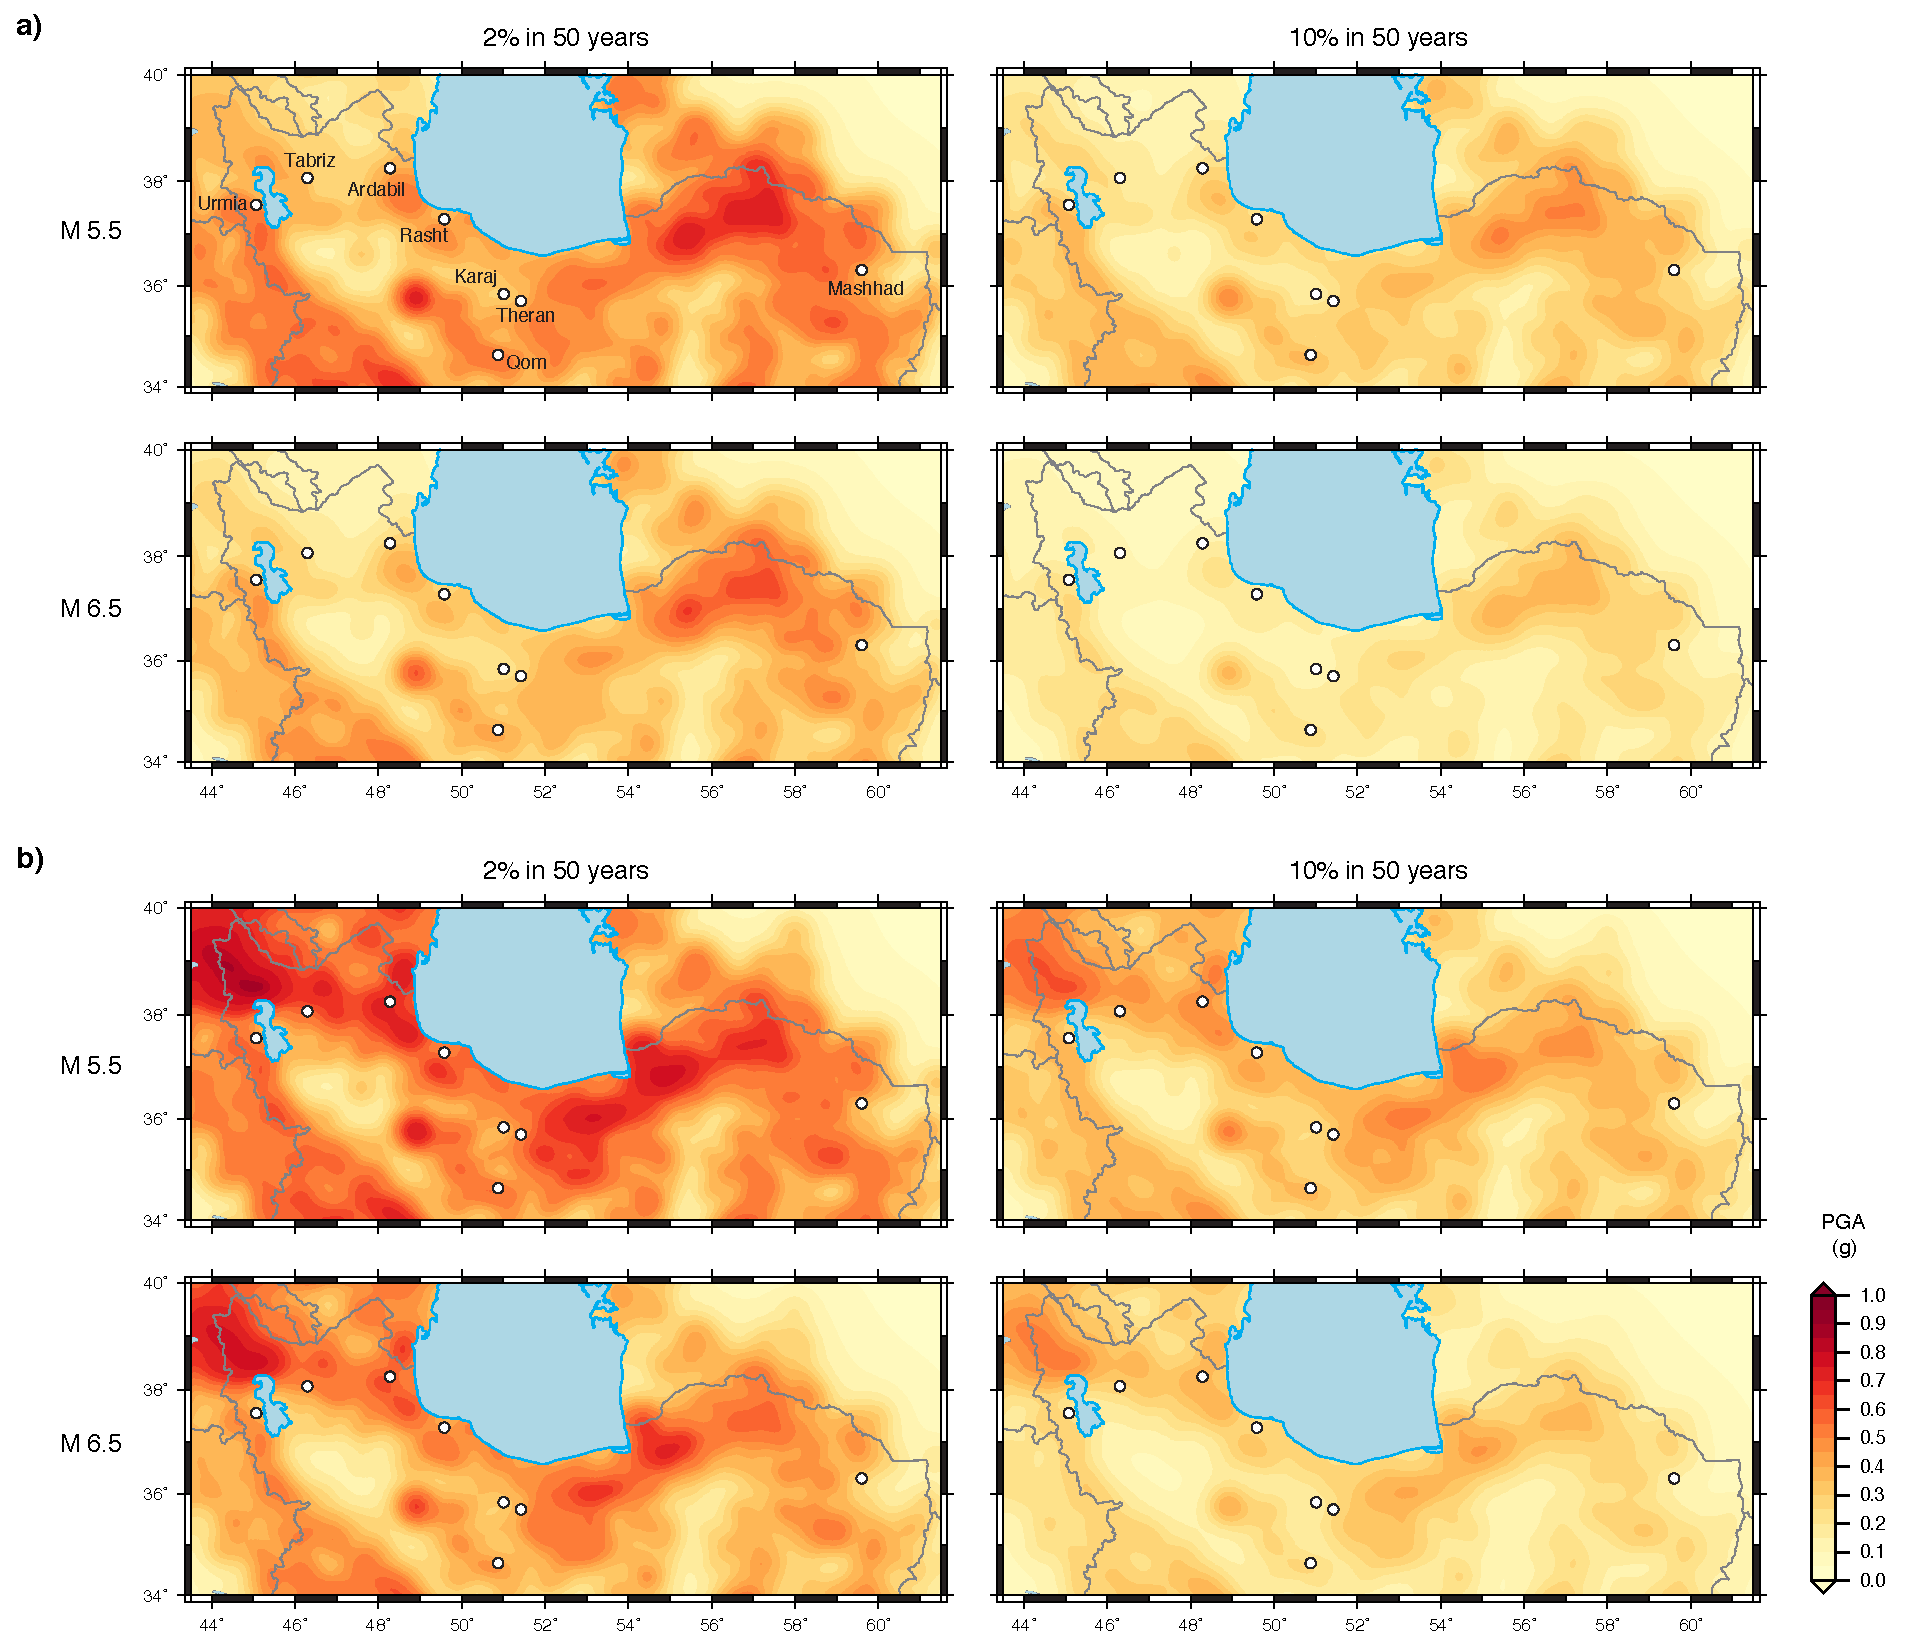
\includegraphics[width=\textwidth]{figures/pdf/figure-08}
    \caption{Variation of horizontal peak ground acceleration (PGA) with distance. KG2004: \citet{Kalkan2004}, BA2008: \citet{Boore2008}, AB2010: \citet{Akkar2010}, SO2012: \citet{Soghrat2012}. The dashed line are $\pm$uncertainty of KG2004.}
    \label{fig:att}
\end{figure*}

\section{Attenuation Relationship}

The last piece in our hazard analysis process is the choice of an adequate attenuation relationship, or ground motion prediction equation (GMPE). This is a highly influential factor because it controls \myrevision{the intensity level at a particular site given an earthquake of a certain magnitude and source characteristics and at a particular distance from the location of interest.}

Recently, \citet{Zafarani2014} investigated the predictive capabilities of a set of nine local, regional, and next generation attenuation (NGA) GMPEs to determine their applicability for northern Iran. They evaluated GMPE predictions against data from 32 earthquakes of magnitudes $M_w$ ranging between 4.7 and 7.4. This included comparisons of PGA and response spectral accelerations (SA) computed from time-series recorded on 163 stations located at epicentral distances of up to 200 km. The evaluation was done using the likelihood (LH) and log-likelihood (LLH) methods of \citet{Scherbaum_2004_BSSA, Scherbaum_2009_BSSA}. The combined evaluation for PGA, and SA for seven periods (T) between 0.1 and 2.0 s, yielded that the best overall predictions were those of the GMPEs introduced by \citet{Ghasemi_2009_JS}, \citet{Abrahamson_2008_ES}, and \citet{Chiou2008}. For the specific case of PGA ($T = 0$ s), however, the best results were those obtained with the GMPEs introduced by \citet{Kalkan2004}, \citet{Chiou2008}, and \citet{Boore2008}. \myrevision{Other GMPEs with good prediction results for the region were those of \citet{Soghrat2012} and \citet{Akkar2010}}.

\myrevision{A common approach used in seismic hazard analysis given the availability of multiple GMPEs is to address the associated epistemic uncertainty through a combination of the various GMPEs. However, in comparisons not shown here for brevity, we found that some of these GMPEs yielded mean predictions that were very close to each other. In an analysis based on the LLH coefficients reported by \citet{Zafarani2014}, and using the approach of \citet{Scherbaum_2009_BSSA} we found, for instance, that a logic-tree partition for the GMPEs proposed by \citet{Kalkan2004}, \citet{Chiou2008}, and \citet{Boore2008}, leads to weights of 0.3376, 0.3354, and 0.3270, respectively. These results meant that neither of these GMPEs had a substantial advantage over the others. This, however, would go against the desired to account for the associated uncertainty. Recently, \citet{Atkinson2014} argued that in such cases where multiple GMPEs do not offer sufficient variability, their combination does not necessarily and properly address uncertainty and suggests that, instead, one can better consider a high and low alternative based on a central backbone model. Fig.~\ref{fig:att} illustrates the variation of horizontal PGA components (in g) with distance obtained using four of the GMPEs mentioned before for two different earthquake magnitudes. In these and other similar comparisons we noticed that the GMPE proposed by \citet{Kalkan2004} led to centered prediction and we chose this particular GMPE as our central backbone and define an upper and lower bound as the two alternative GMPEs in our logic tree analysis, such that---for the most part---the amplitudes predicted by the mean values of other GMPEs fell within the range of defined by these bounds.}

The selected the GMPE proposed by \citet{Kalkan2004} for our analysis is of the form
%
\begin{align}
	\ln \left( Y \right) =
		& \hspace{1ex} b_1 + b_2(M_w - 6) + b_3 \left( M_w - 6 \right)^{2} \nonumber \\
		& + b_5 \ln \left( r \right) + b_V \ln \left( V_S / V_A \right)
	\, ,
\end{align}
%
where $Y$ is a ground motion parameter (here representing PGA), $V_A$ is a reference velocity in m/s, \myrevision{and} $V_S$ is the shear wave velocity of the site of interest. In this equation, the distance $r$ is given by
%
\begin{equation}
	r= \sqrt{ r^2_{\mathit{cl}} + h^2 }
	\, ,
\end{equation}
%
where $r_{\mathit{cl}}$ is the horizontal distance to the site of interest and $h$ is a reference fictitious depth, both given in km. According to \citet{Kalkan2004}, in the case of $Y$ representing PGA, the coefficients $b_1$, $b_2$, $b_3$, $b_5$ and $b_V$ are
%
\begin{equation}
\begin{array}{lcrlcr}
	b_1 &=&  0.393   \,,&\hspace{2em}   b_2 &=& 0.576\,,   \\
	b_3 &=& -0.107   \,,&\hspace{2em}   b_5 &=& -0.899\,,  \\
	b_V &=& -0.200   \,;
	\nonumber
\end{array}
\end{equation}
%
and $V_A$, $V_S$ and $h$ are
%
\begin{equation}
\begin{array}{lcrl}
	V_A &=& 1,112 & \mathrm{m/s}	\\
	V_S &=&   700 & \mathrm{m/s}	\\
	h   &=&  6.91 & \mathrm{km}\,,
	\nonumber
\end{array}
\end{equation}
%
respectively. The standard deviation of the residuals $(\sigma_{\ln y})$ expressing the random variability of the ground motions is 0.612. The value of $V_S$ is assumed to represent average surface rock sites.

We should note here that even though \citet{Kalkan2004} derived the above attenuation relationship for distances $r$ up to 250 km, \citet{Zafarani2014} only used data up to 200 km in their evaluation of the various GMPEs available. Therefore, to be consistent with the latter, we set the models in the hazard analysis to compute ground motion intensities (i.e., PGAs) at distances no greater than 200 km.

% STUFF...

% \myrevision{While other GMPEs were included in the analysis by \citet{Zafarani2014} which also proved to be adequate for the region for other intensity parameters, given our focus on PGA, we concentrated our attention in the above mentioned equations, with particular attention to \citet{Kalkan2004}, \citet{Boore2008}, \citet{Soghrat2012} and \citet{Akkar2010}.}

% In practice, epistemic uncertainty is considered by using different GMPEs through logic tree approach. As \citet{Atkinson2014} suggested, in most cases multiple-GMPEs approach is not necessarily acknowledge the epistemic uncertainty. This fact is also obvious from the Fig.~\ref{fig:att} where the alternative approach which is using \citet{Kalkan2004} as a backbone GMPE as well as uncertainties covers a broader range in compare with using the combination of GMPEs.} Furthermore, based on the LLH coefficients reported by \citet{Zafarani2014}, and using the \myrevision{approach} of \citet{Scherbaum_2009_BSSA}, we found that a logic-tree analysis \myrevision{leads} to weights of 0.3376, 0.3354, and 0.3270 for \citet{Kalkan2004}, \citet{Chiou2008}, and \citet{Boore2008}, respectively.

% \myrevision{Fig.~\ref{fig:logic} represents the total logic tree approach in order to consider the uncertainty in tectonic seismic region, $M_{max}$, $b-value$, and estimated PGA. The weights are chosen based on previous studies \citep[e.g.,][]{Petersen2015}. We considered the uncertainty in tectonic seismic region through adding the uniform model with lower weight than the most recent accepted classification.}


% \section{Old Analysis Parameters Section}

\subsection{b-value}

\textcolor{red}{
[Legacy text to be discussed with Naeem...]\\
}

\textcolor{blue}{
\citet{Karimiparidari2013} applied the Maximum Curvature (MAXC) technique \citep{Wyss1999, Wiemer2000} by ZMap \citep{Wiemer2001} to calculate the level of completeness of instrumental part of the catalog.  Following the \citet{Karimiparidari2013}, we assume the catalog is complete for earthquakes with magnitude 4.5, 4.4, 4.5, 4.5, and 4.4 for Azerbaijan, Alborz,  Kopeh-Dagh, Central Iran, and Zagros tectonic seismic regions, respectively. For the uniform model we used 4.5 as a completeness magnitude. In this study we use those magnitudes of completeness as the magnitude threshold in the calculation of the seismicity parameters. We also used the seismicity parameters of \citet{Karimiparidari2013} as the priory information in HA3 code. The updated values are displayed in Table \ref{tab:b_value}.  Annual occurrence rate of the earthquake for each region is shown in Fig.~\ref{fig:annual_m}.
}

\subsection{Catalog Completness}

For the smoothed seismicity method, completeness of each magnitude in the catalog is an important factor.  \citet{Frankel1995} plotted the cumulative number of events against time for different regions. He assumes that from the point that the line become linear, the catalog is complete. This approach is similar to the MAXC method of ZMAP software \citep{Wiemer2001}, where the completeness treshold is the maximum value of the first derivative of the frequency-magnitude curve. Using the cumulative frequency-magnitude distribution of \citet{Gutenberg1944} and also frequency magnitude distribution approach in software ZMAP, \citet{Zare2014} reported the catalog completeness for the study regions. World widely large earthquakes were routinely located after increasing number of seismic stations establishment in the early 1900s \citep{Shearer2009}. Up to 1961 these data formed the early instrumental period. In 1961 the Worldwide Standardized Seismograph Network (WWSSN) was stablished. The record of these seismographs considerably improved the seismic catalogs in different part of the world \citep{Shearer2009}. Fig.~\ref{fig:completness_scatter} shows the magnitude distribution of events with respect to the time of occurrence of the events.

% \begin{figure*} [!ht]
% \centering
% 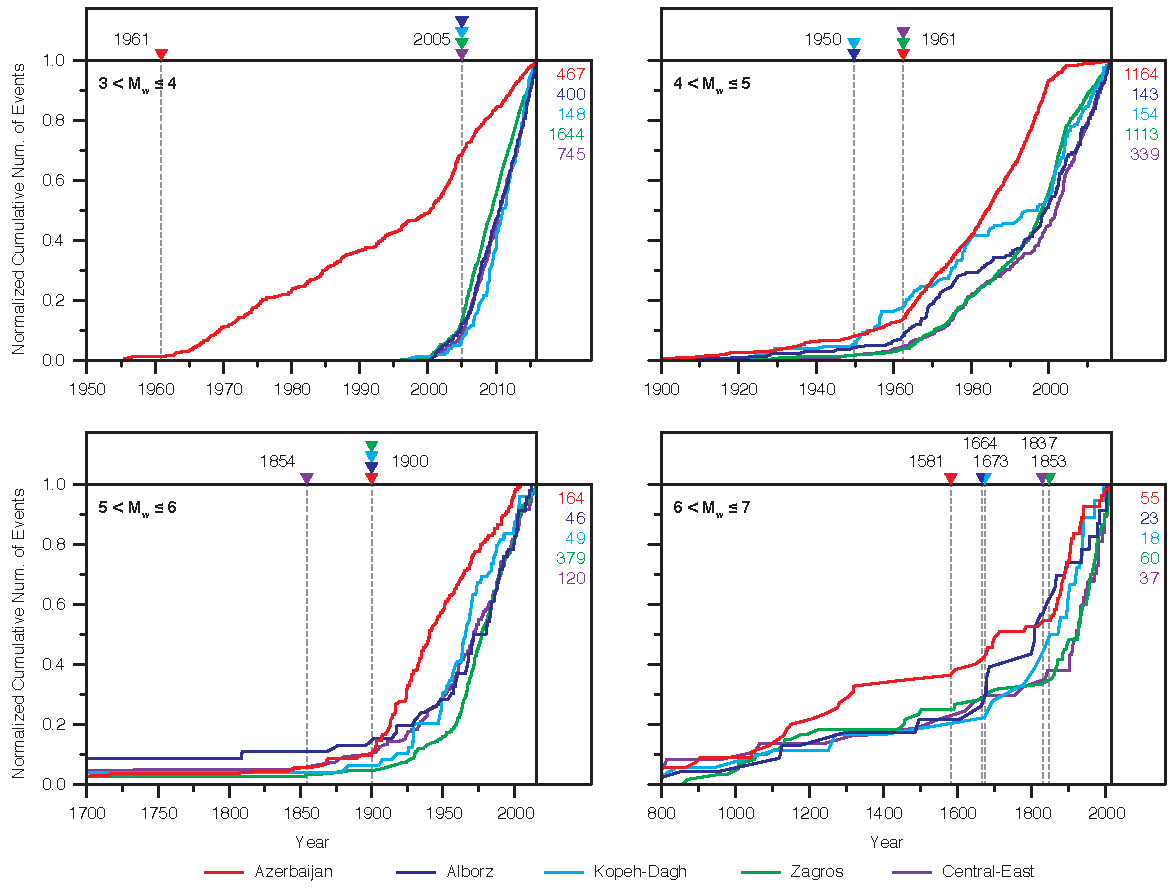
\includegraphics[scale=0.5]{figures/pdf/figure-05.pdf} 
% \caption{Magnitude-time distribution of earthquakes in the study regions. a) Alborz, b) Azerbaijan, c) Central, d) Kopeh Dagh, e) Uniform f) Zagros}
% \label{fig:completness_scatter}
% \end{figure*}

According to   \citet{Frankel1995},  we made plots of the cumulative number of events against time for different regions' catalog. We pick the Mw 0.5 increments in magnitude to be able to compare the results with \citet{Zare2014}. In order to be able to compare the results with \citet{Zare2014} we merge the data of Azerbaijan and Alborz seismic regions.  Fig.~\ref{fig:completness_compare_zare_2014_Az_Al} shows the completeness of catalog for earthquakes with different magnitude range in Azerbaijan-Alborz region. According to this figure, midrange magnitudes ($ 4 < Mw < 6 $) fairly obey the network developments in 1900 and 1961. The completeness thresholds for each magnitude range which are reported by \citet{Zare2014} are shown by dashed green line. In this study we follow the \citet{Frankel1995} approach to determine the completeness of each region. Even though the approach used by \citet{Frankel1995} will lead to the conservative results, we make sure that we don't use a period of time without knowing the complete number of events. Determining the completeness of the catalog is very sensitive to the data. Converting earthquake magnitudes from different scales to moment magnitude obviously has some error. Having broader range of magnitude will help to minimize these sort of error. In this study we consider the magnitude intervals for completeness study as $Mw = 1$. 

% \begin{figure*} [!ht]
% \centering
% 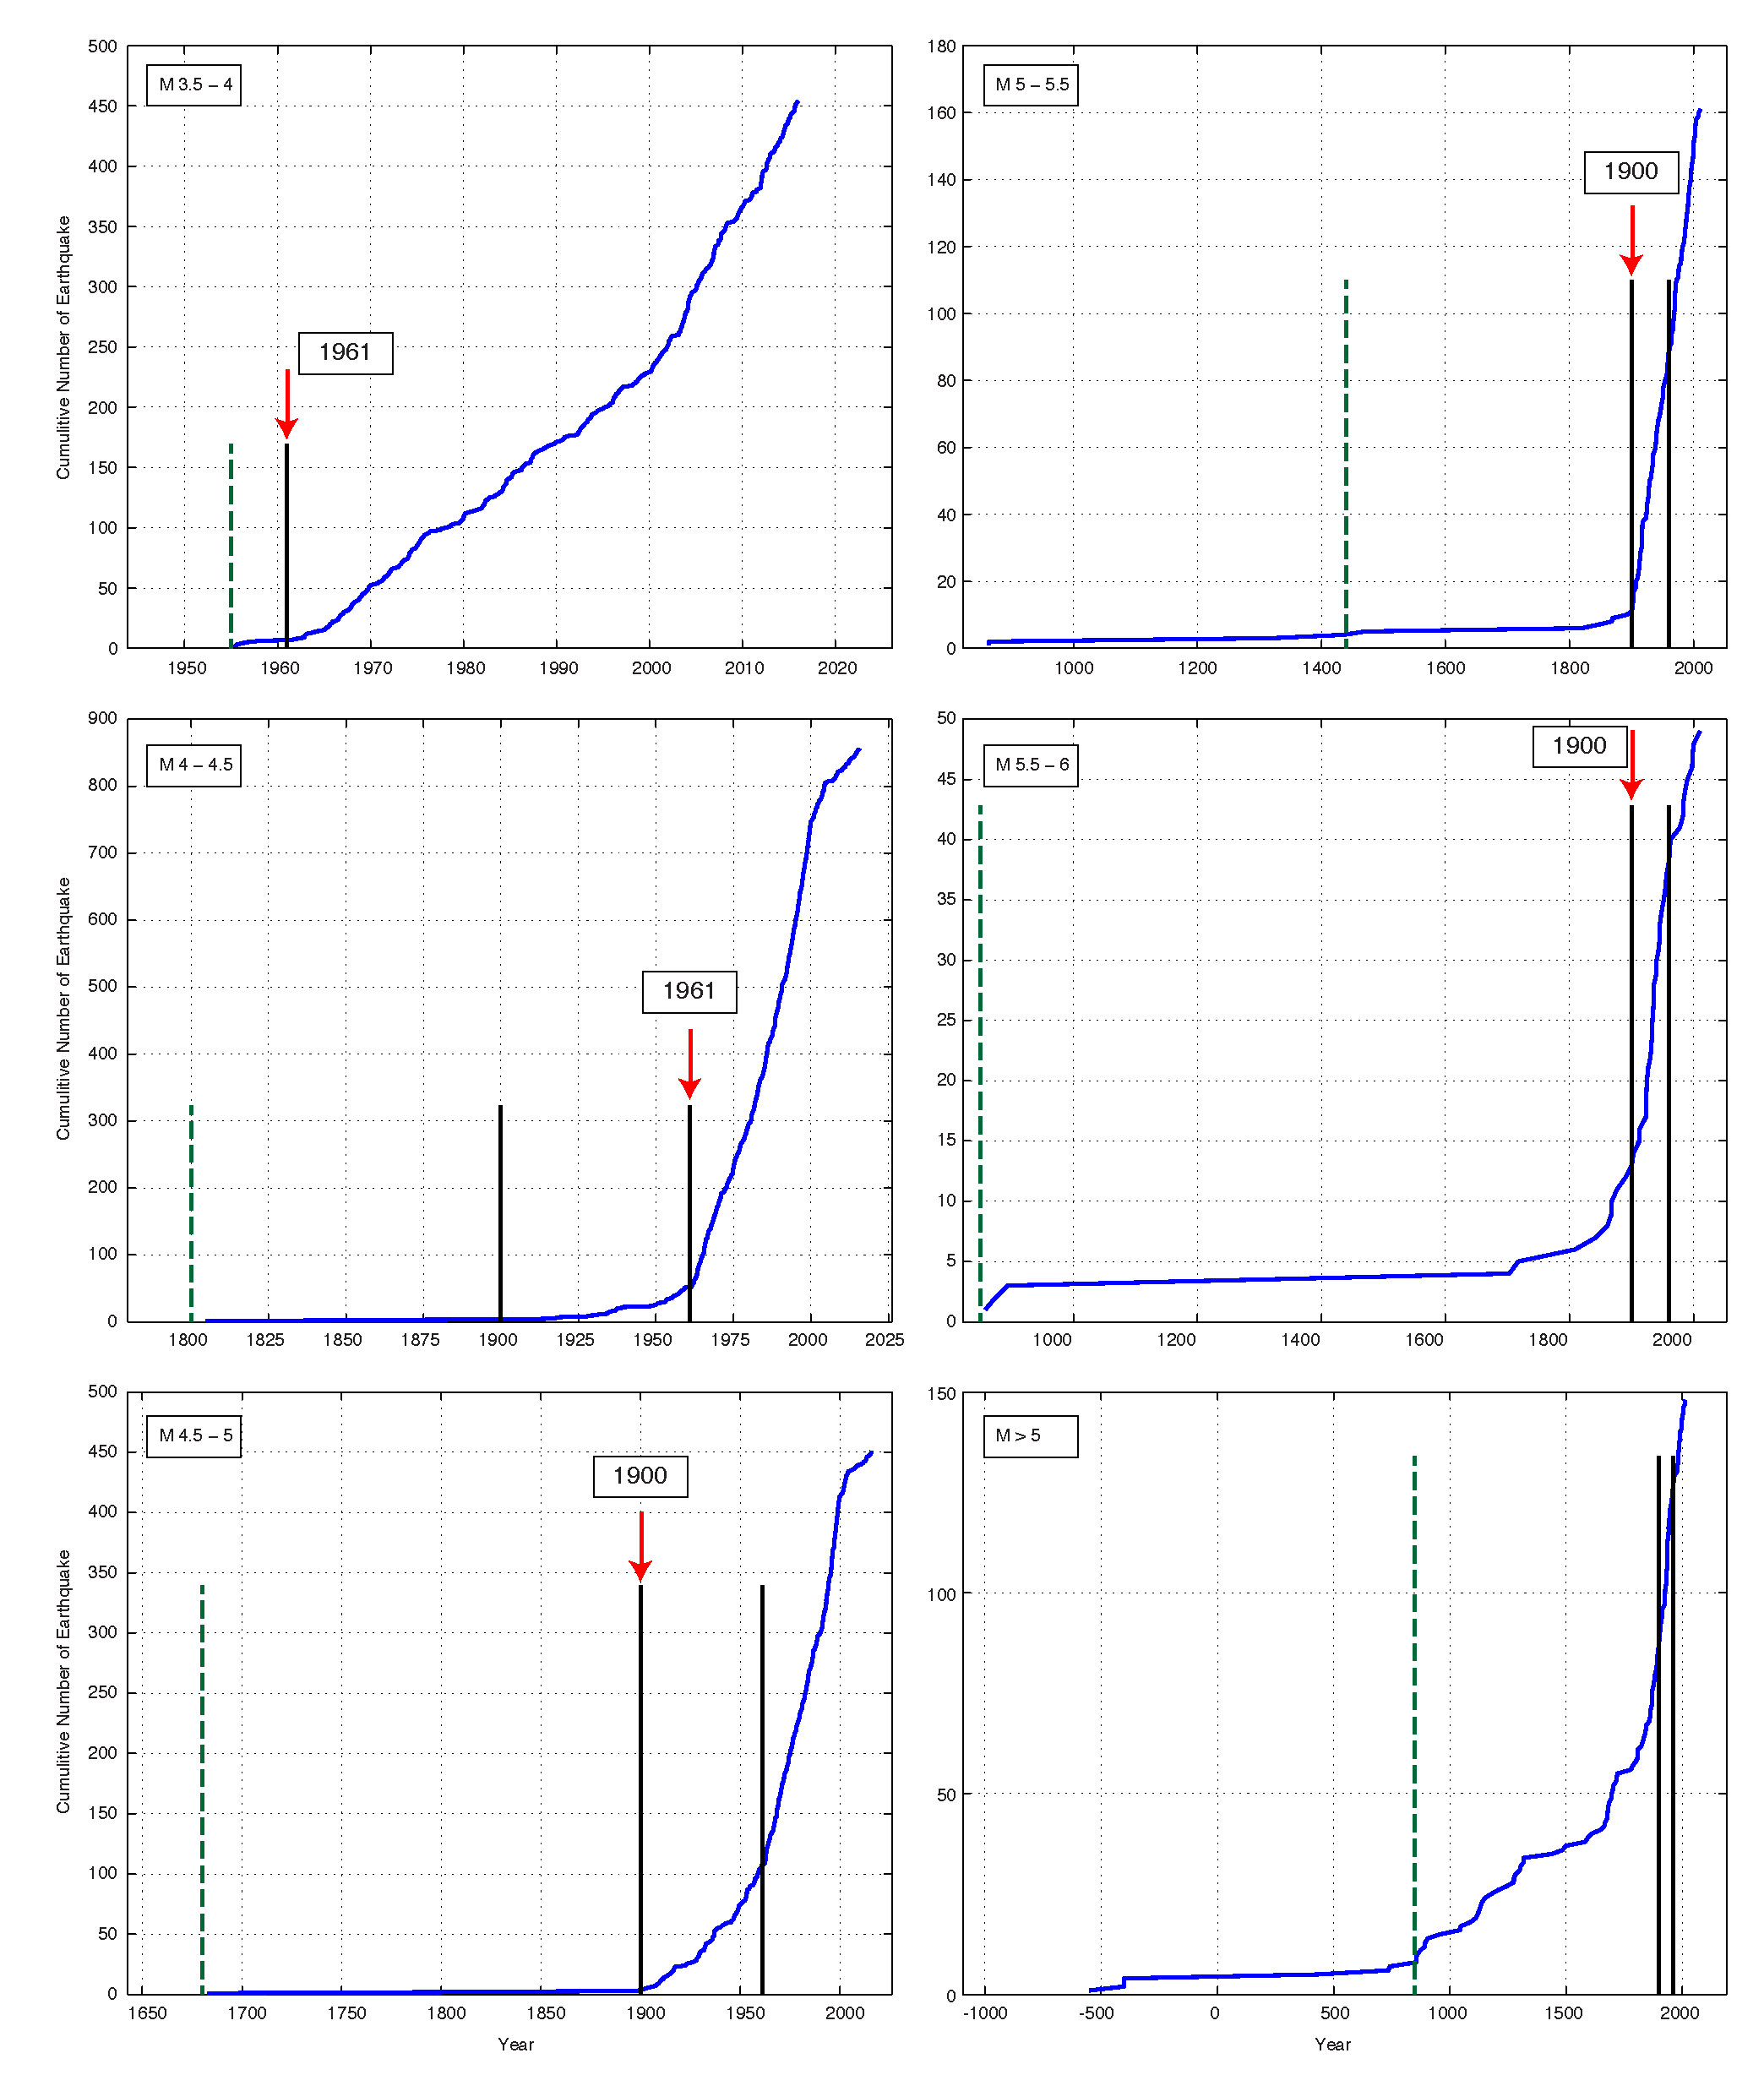
\includegraphics[scale=0.4]{figures/pdf/completness_compare_zare_2014_Az_Al.pdf} 
% \caption{Cumulative number of earthquakes with respect to the time. Magnitude range is represented in a box at the top left corner. Solid black lines represent the starting of early instrumental (1900) and instrumental (1961) period. Green dashed lines represents the completeness threshold reported by \citet{Zare2014}. Arrows show the possible places to choose as completeness threshold after \citet{Frankel1995}.}
% \label{fig:completness_compare_zare_2014_Az_Al}
% \end{figure*}

\noindent
Fig.~\ref{fig:comp_test_all_mag} illustrates the completeness of data for each magnitude threshold in five different regions. A uniform rise of cumulative number of earthquake in each magnitude range, defines the threshold for catalog completeness. We define the completeness of each magnitude range at a time which the cumulative number of earthquake increase linearly with time. We assume the catalog for earthquakes with magnitude greater than  7 ($M_w > 7$) is complete from the first historical earthquake report.  Determining the completeness of the catalog for $ 6 < Mw \leq 7 $ needs precise observation of the catalog. In Azerbaijan tectonic seismic region after 1045  $Mw = 6.2$ earthquake the catalog seems complete up to 1318. However, between 1318 and 1581 (263 years) only one earthquake with magnitude $Mw > 6$ is reported (1440,  $Mw = 6.2$ ). Considering the activity of the Azerbaijan region, in this study we assume that the catalog is complete for earthquake with magnitude $ 6 < Mw \leq 7 $ after 1581. Similar situation happened at the period of 1715 - 1833. It worth to mention that in this case, the time period is shorter than before (118 years), meanwhile in this period of time two earthquakes with magnitude $Mw>7$ occurred in the Azerbaijan region (1721 $Mw=7.7$, 1780 $Mw=7.6$). The catalog may or may not be completed after 1045, however in this study we consider 1581 as a completeness threshold for magnitude  $ 6 < Mw \leq 7 $. Considering completeness of the catalog for Azerbaijan region from 1581 will result in conservative PGA for the region in comparison with the model with threshold of 1045. We picked the completeness threshold for other regions and other magnitude ranges according as a year that the cumulative number of earthquakes increment uniformly. Table ~\ref{tab:completeness} shows the summary of values used in this study.


% \begin{figure*} [!ht]
% \centering
% 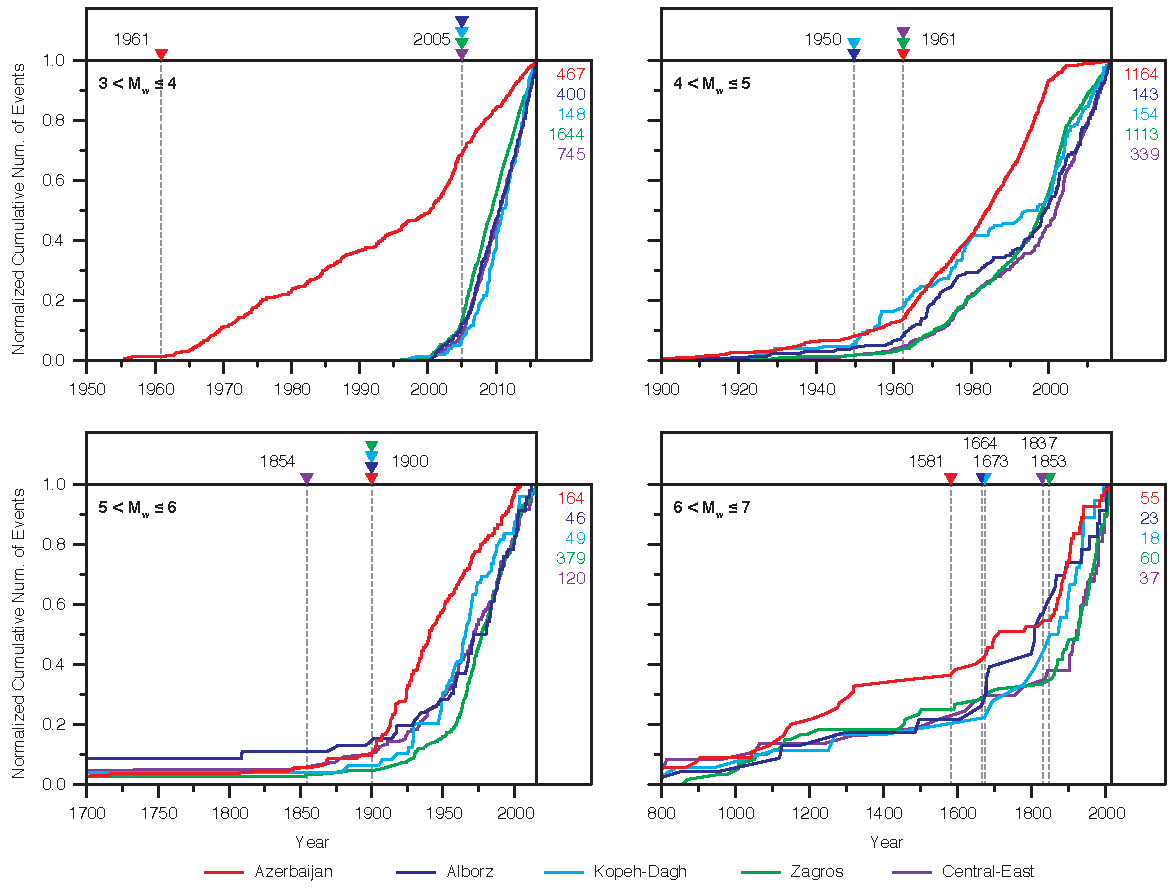
\includegraphics[scale=0.28]{figures/pdf/figure-05.pdf} 
% \caption{Magnitude-time distribution of earthquakes in the study regions. a-b) Alborz, c-d) Azerbaijan, e-f)Central, g-h)Kopeh Dagh, i-j)Zagros}
% \label{fig:comp_test_all_mag}
% \end{figure*}



% \begin{table*}[!ht]
% \centering
% \caption{Completeness threshold of tectonic seismic regions.}
% \begin{tabular}{ccccccccc}
%  ~           & Azerbaijan & Alborz & Kopeh Dagh & Central Iran & Zagros & North Iran  \\ \hline
% 3-4         & 1961          & 2005   & 2005             & 2005            & 2005    & 2005          \\ \hline
% 4-5         & 1961          & 1961   & 1950             & 1961            & 1961    & 1961          \\ \hline
% 5-6         & 1900          & 1900   & 1900             & 1854            & 1900    & 1900           \\ \hline
% 6-7         & 1581          & 1664   & 1673             & 1837            & 1853    & 1778           \\ \hline
% 7 $< $    & 1042          & -401    & 9                   & 762              & 1439    & -401            \\ 
% \end{tabular}
% \label{tab:completeness}
% \end{table*}














%% ---------------------------------------------
%% ---------------------------------------------
%
%% My (Naeem) original text.
%
%
%\section{Analysis Parameters}
%%\subsection{Magnitude Interval}
%%\subsection{Minimum Magnitude}
%\subsection{Attenuation Relationship}
%The choice of a ground motion attenuation model is of great importance since attenuation has proven to be a highly influential factor of seismic hazard. \citet{Zafarani2014} used 163 free-field acceleration time histories recorded at epicentral distance of up to 200 km from 32 earthquakes to investigate the predictive capabilities of the local, regional, and next generation attenuation (NGA) ground-motion prediction equations and determined their applicability for northern Iran. After evaluating different Ground Motion Prediction Equations, \citet{Kalkan2004}, \citet{Chiou2008}, and \citet{Boore2008} represented suitable performance for  PGA  with LLH (Log-Likelihood method) score of 1.54, 1.55, and 1.59. Mean of the mentioned attenuation relationships (not shown here), are very close together, especially at higher magnitude. Using \citet{Scherbaum2009} approach and \citet{Zafarani2014} coefficients we calculated the logic tree weights as 0.3376, 0.3354, and 0.3270, respectively. Getting close mean values and logic tree weights, in order to consider the epistemic uncertainty, instead of using several GMPEs we use the top rank GMPE (i.e.  \citet{Kalkan2004} ). We also presented the results for  $\pm$ standard deviation. \\
%
%\noindent
%The attenuation relationship is:
%
%\begin{equation}
%\begin{split}
%ln\ (Y) = b_1 + b_2(M_w-6) + b_3( M_w-6)^{2}+  \\ 
%b_5ln\ r + b_V \ ln(V_S/V_A) \  with \  r= \sqrt{R{r^2_{cl} + h^2}}  
%\end{split}
%\end{equation}
%
%where $Y$ is in $g$, $b_1 = 0.393$, $b_2 = 0.576$, $b_3 = -0.107$, $b_5 = -0.899$, $b_V = -0.200$, $V_A = 1112$, $h(km) = 6.91$, $\sigma_{ln\ Y} = 0.612$.
%
%\subsection{b-value}
%
%For each of the three seismic regions, Gutenberg-Richter parameters and Max magnitude ($M_{max}$) were calculated using Seismic Hazard Assessment code (HA3) \citep{kijko2004}. The regional maximum magnitude for each region is estimated by the \citet{Kijko1989} method, which is implemented in the HA3 package. For smoothed seismicity areas, $b-value$ is assumed constant. The $a-value$ can vary spatially and is determined by counting earthquakes above $M$ 3.0 in each grid cells.\\
%\noindent
%\citet{Karimiparidari2013} applied the Maximum Curvature (MAXC) technique \citep{Wyss1999, Wiemer2000} by ZMap \citep{Wiemer2001} to calculate the level of completeness of instrumental part of the catalog.  Following the \citet{Karimiparidari2013}, we assume the catalog is complete for earthquakes with magnitude 4.5, 4.4, 4.5, 4.5, and 4.4 for Azerbaijan, Alborz,  Kopeh-Dagh, Central Iran, and Zagros tectonic seismic regions, respectively. For the north Iran uniform model we used 4.5 as a completeness magnitude. In this study we use those magnitudes of completeness as the magnitude threshold in the calculation of the seismicity parameters. We also used the seismicity parameters of this study \citep{Karimiparidari2013} as the priory information in HA3 code. The updated values are displayed in Table \ref{tab:b_value}.  Annual occurrence rate of the earthquake for each region is shown in Fig.~\ref{fig:annual_m}.
%
%\begin{figure*} [!ht]
%\centering
%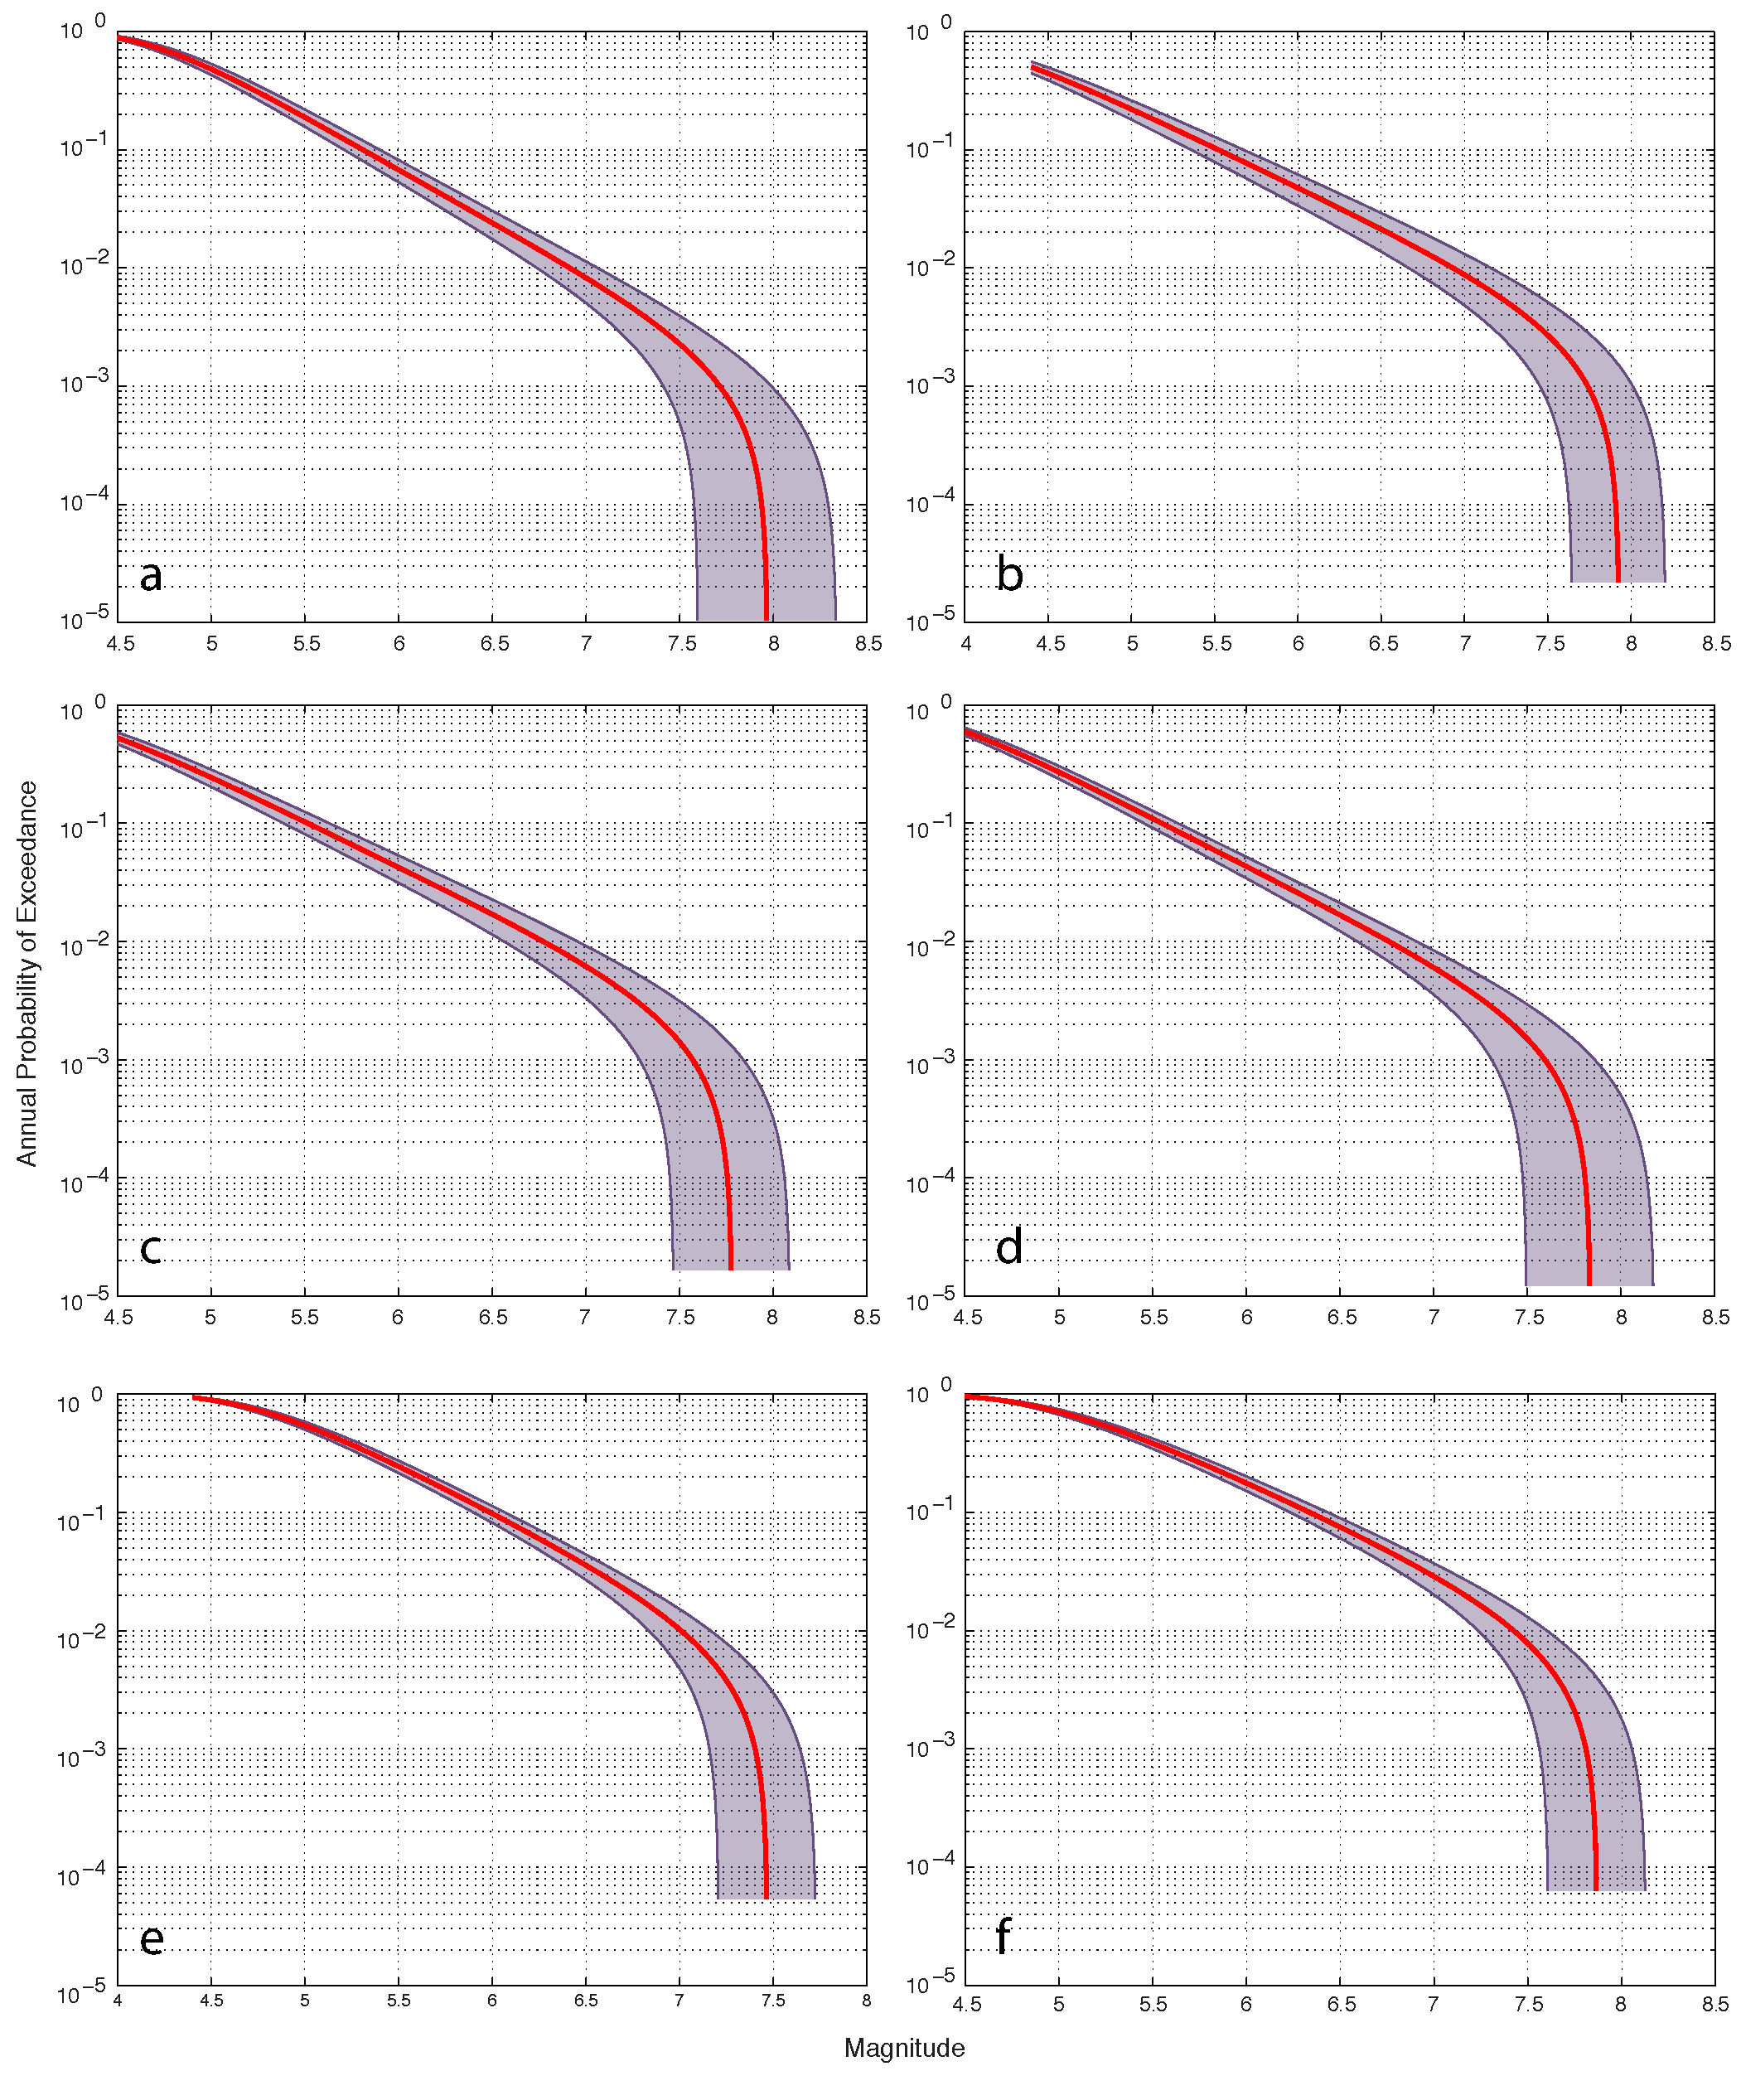
\includegraphics[scale=0.4]{figures/pdf/annual_rate_m.pdf} 
%\caption{Annual occurrence rate of the earthquake. a) Azerbaijan, b) Alborz, c) KopehDagh, d)Central, e)Zagros f) North Iran}
%\label{fig:annual_m}
%\end{figure*}
%
%
%
%
%\noindent
%
%
%\begin{table*}[!ht]
%\centering
%\caption{Seismicity parameters for three tectonic seismic regions.}
%    \begin{tabular}{ccccc}
%    ~                          &         $b-value$     &   $M_{max} $  Calculated & $M_{max}$ obseved \\ \hline
%    Azerbaijan           & 1.1   $\pm$ 0.03   &   7.93  $\pm$  0.34           &   7.7      			    \\ \hline
%    Alborz                  &1.03  $\pm$ 0.03   &   7.85  $\pm$  0.66           &   7.8          	            \\ \hline
%    Kopeh Dagh        & 0.89 $\pm$ 0.04   &   7.78  $\pm$  0.31           &   7.6          	            \\ \hline
%    Central Iran         & 0.95 $\pm$ 0.04   &   7.84  $\pm$  0.34           &   7.6                           \\ \hline
%    Zagros                 & 0.99 $\pm$ 0.02  &   7.47  $\pm$  0.26            &  7.4                            \\ \hline
%    Uniform Model    & 0.9    $\pm$ 0.02  &   7.87  $\pm$  0.26            &  7.8                            \\ 
%    \end{tabular}
% \label{tab:b_value} 
%\end{table*}
%
%
%\subsection{Catalog Completness}
%For the smoothed seismicity method, completeness of each magnitude in the catalog is an important factor.  \citet{Frankel1995} plotted the cumulative number of events against time for different regions. He assumes that from the point that the line become linear, the catalog is complete. Using the cumulative frequency-magnitude distribution of \citet{Gutenberg1944} and also frequency magnitude distribution approach in software ZMAP \citep{Wiemer2001}, \citet{Zare2014} reported the catalog completeness for the study regions. World widely large earthquakes were routinely located after increasing number of seismic stations establishment in the early 1900s \citep{Shearer2009}. Up to 1961 these data formed the early instrumental period. In 1961 the Worldwide Standardized Seismograph Network (WWSSN) was stablished. The record of these seismographs considerably improved the seismic catalogs in different part of the world \citep{Shearer2009}. Fig.~\ref{fig:completness_scatter} shows the magnitude distribution of events with respect to the time of occurrence of the events.
%
%\begin{figure*} [!ht]
%\centering
%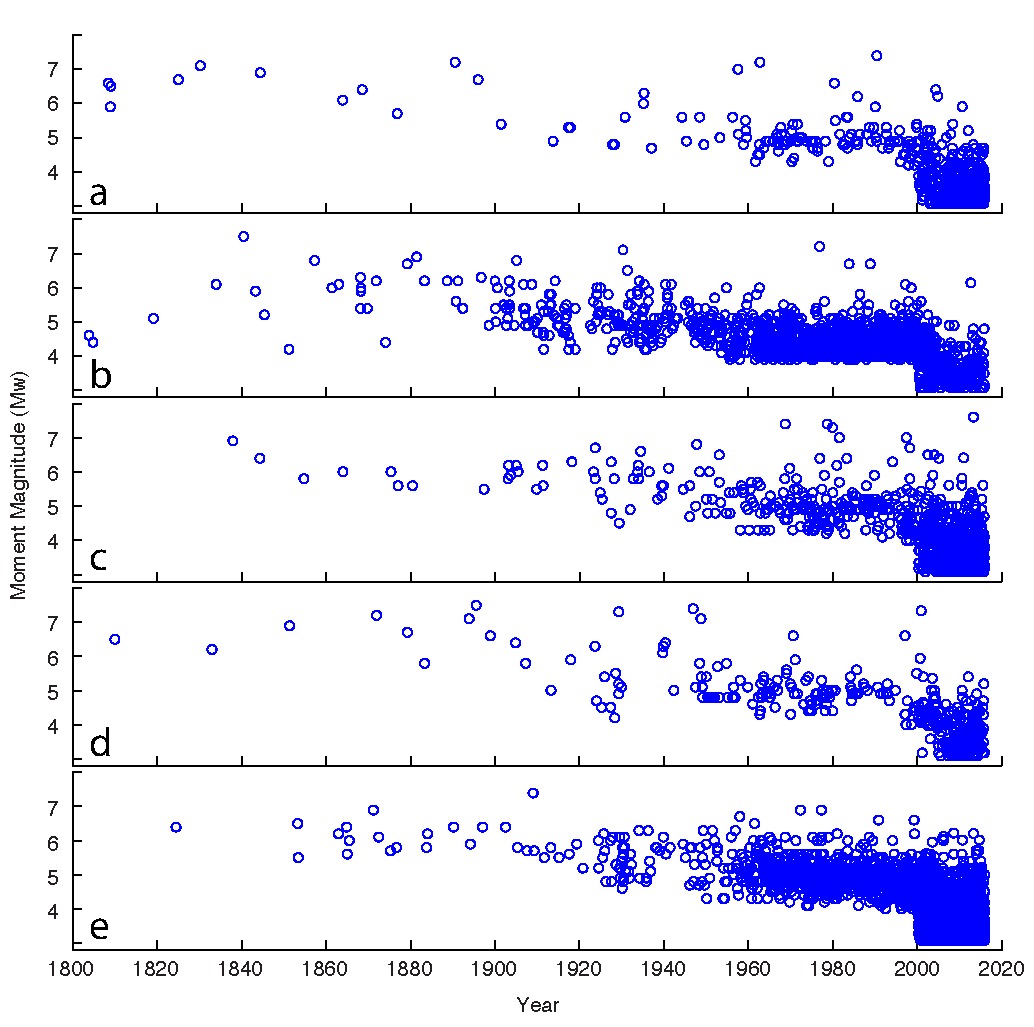
\includegraphics[scale=0.6]{figures/pdf/completness_scatter.pdf} 
%\caption{Magnitude-time distribution of earthquakes in the study regions. a) Alborz, b) Azerbaijan, c)Central, d)Kopeh-Dagh, e)Zagros}
%\label{fig:completness_scatter}
%\end{figure*}
%
% According to   \citet{Frankel1995},  we made plots of the cumulative number of events against time for different regions' catalog. We pick the Mw 0.5 increments in magnitude to be able to compare the results with \citet{Zare2014}. In order to be able to compare the results with \citet{Zare2014} we merge the data of Azerbaijan and Alborz seismic regions.  Fig.~\ref{fig:completness_compare_zare_2014_Az_Al} shows the completeness of catalog for earthquakes with different magnitude range in Azerbaijan-Alborz region. According to this figure, midrange magnitudes ($ 4 < Mw < 6 $) fairly obey the network developments in 1900 and 1961. The completeness thresholds for each magnitude range which are reported by \citet{Zare2014} are shown by dashed green line. In this study we follow the \citet{Frankel1995} approach to determine the completeness of each region. Even though the approach used by \citet{Frankel1995} will lead to the conservative results, we make sure that we don't use a period of time without knowing the complete number of events. Determining the completeness of the catalog is very sensitive to the data. Converting earthquake magnitudes from different scales to moment magnitude obviously has some error. Having broader range of magnitude will help to minimize these sort of error. In this study we consider the magnitude intervals for completeness study as $Mw = 1$. 
%
%\begin{figure*} [!ht]
%\centering
%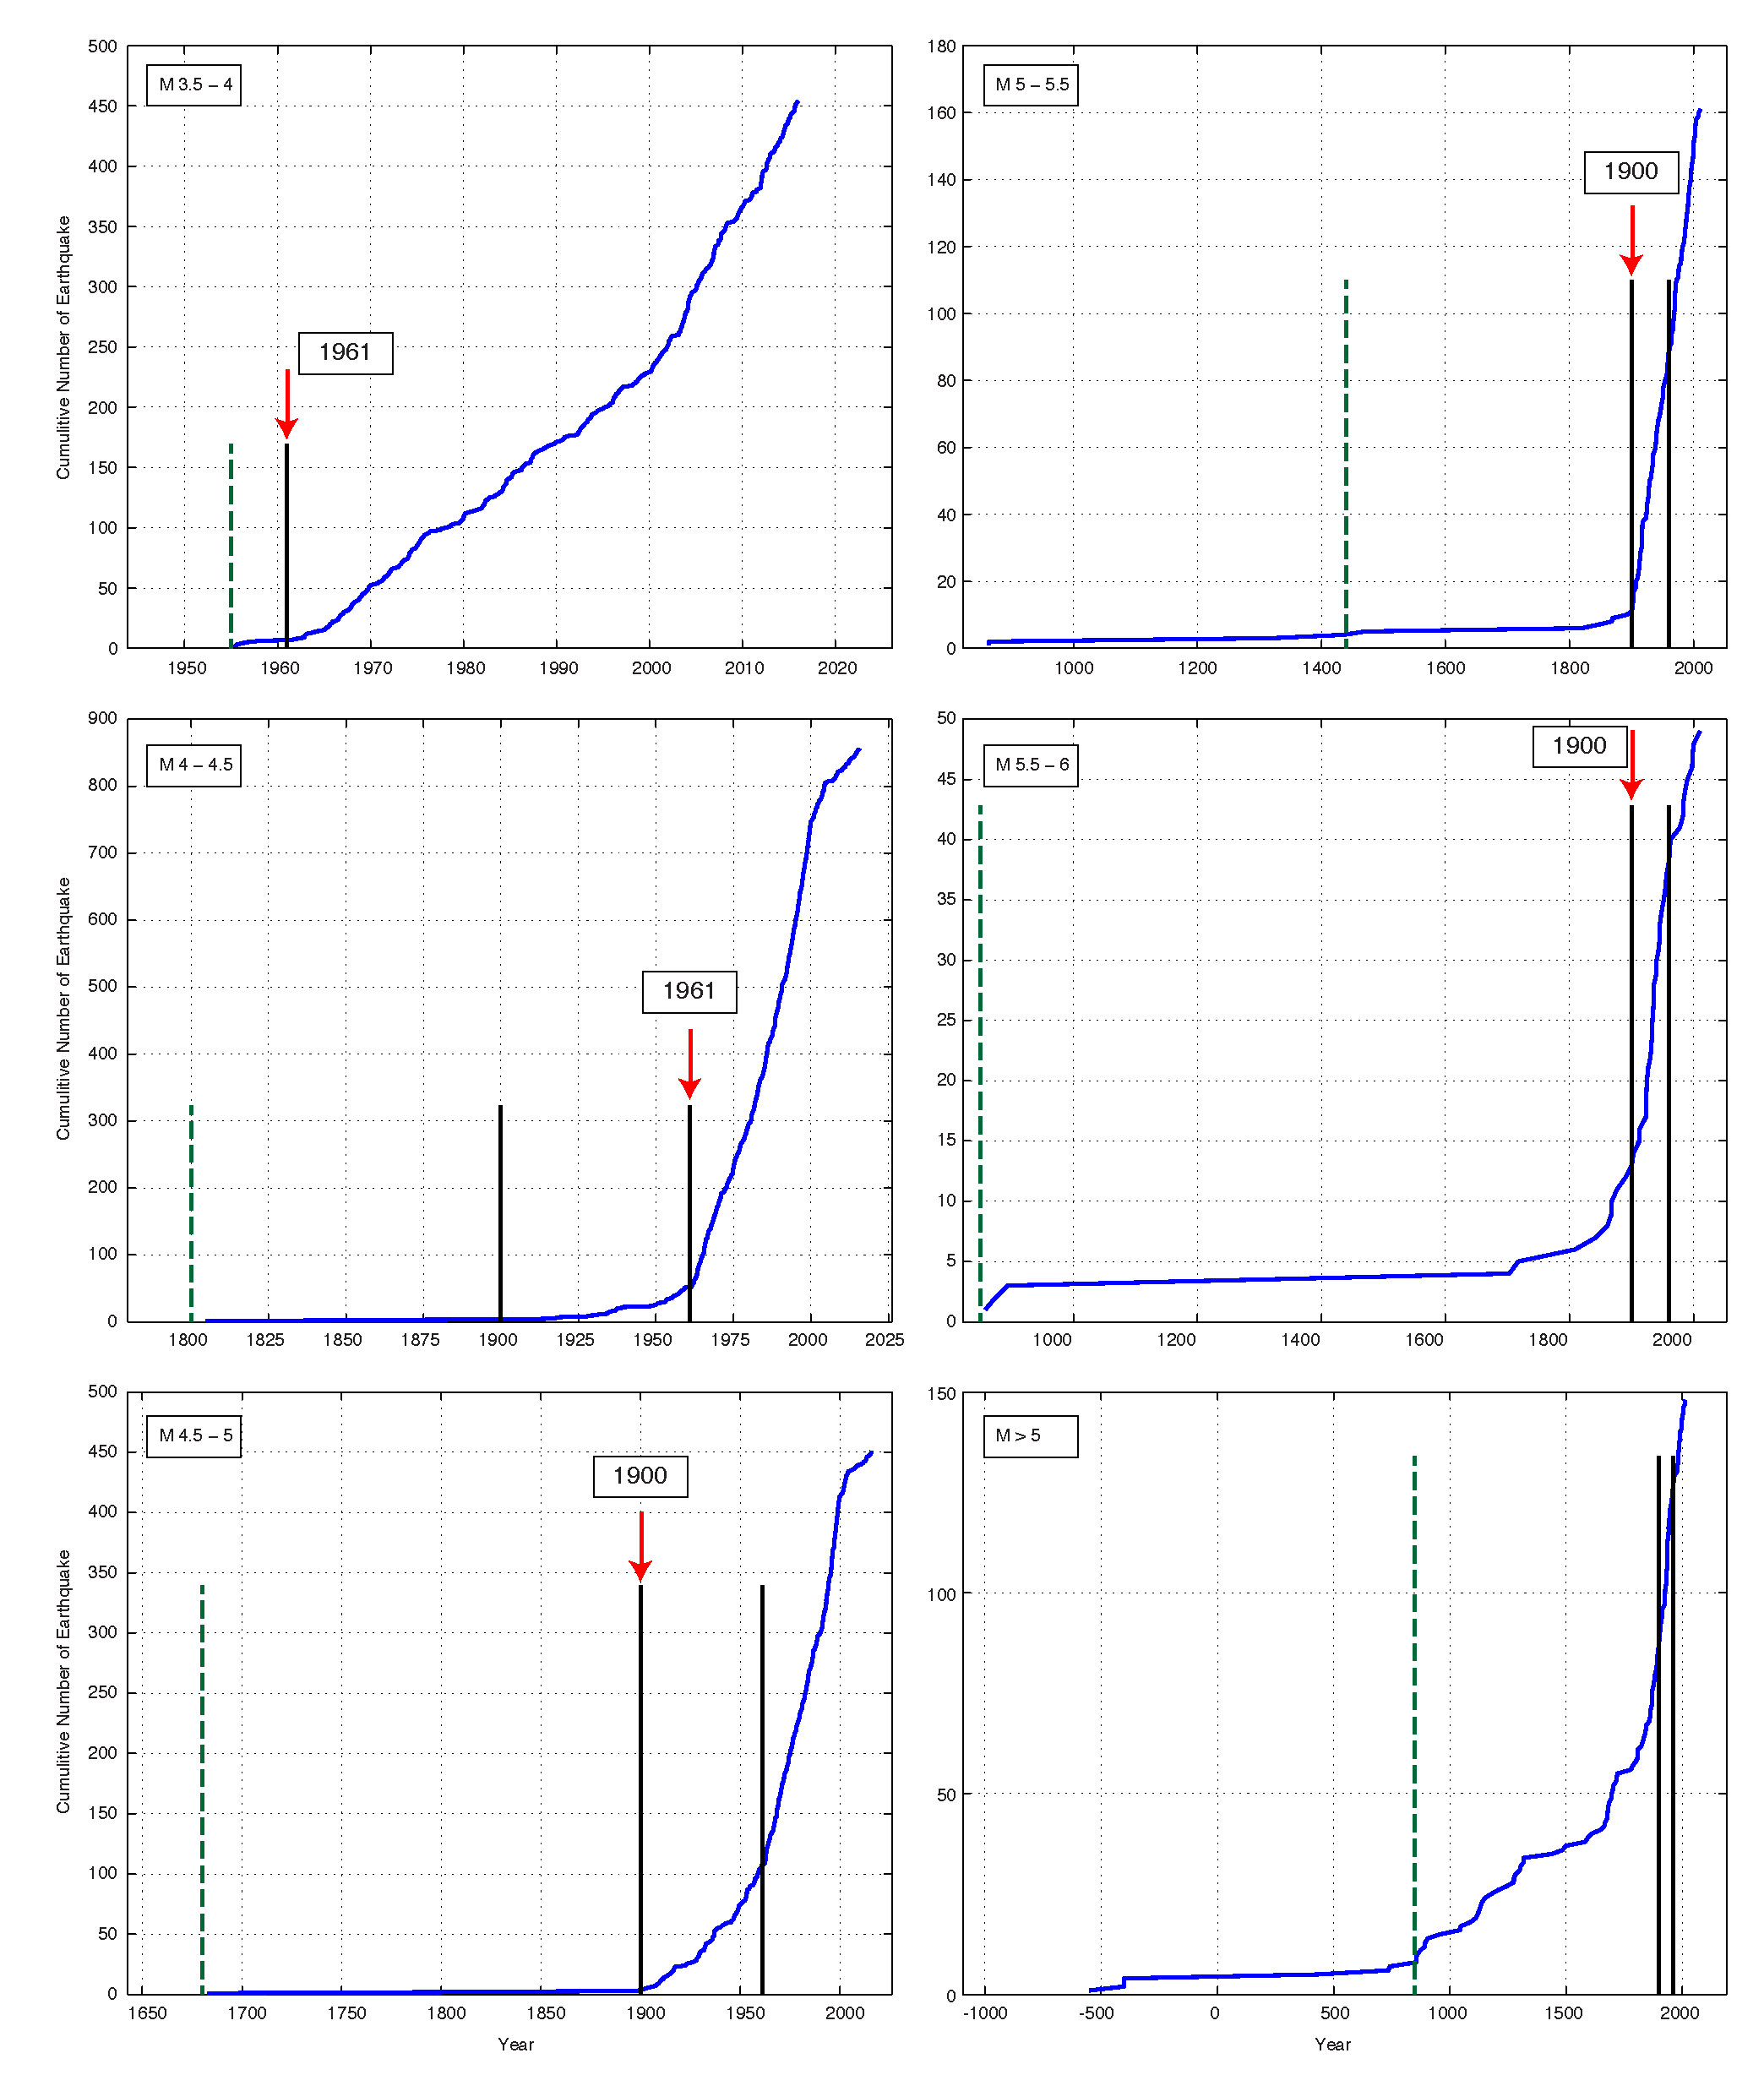
\includegraphics[scale=0.4]{figures/pdf/completness_compare_zare_2014_Az_Al.pdf} 
%\caption{Cumulative number of earthquakes with respect to the time. Magnitude range is represented in a box at the top left corner. Solid black lines represent the starting of early instrumental (1900) and instrumental (1961) period. Green dashed lines represents the completeness threshold reported by \citet{Zare2014}. Arrows show the possible places to choose as completeness threshold after \citet{Frankel1995}.}
%\label{fig:completness_compare_zare_2014_Az_Al}
%\end{figure*}
%
%\noindent
%Fig.~\ref{fig:comp_test_all_mag} illustrates the completeness of data for each magnitude threshold in five different regions. A uniform rise of cumulative number of earthquake in each magnitude range, defines the threshold for catalog completeness. We define the completeness of each magnitude range at a time which the cumulative number of earthquake increase linearly with time. We assume the catalog for earthquakes with magnitude greater than  7 ($M_w > 7$) is complete from the first historical earthquake report.  Determining the completeness of the catalog for $ 6 < Mw \leq 7 $ needs precise observation of the catalog. In Azerbaijan tectonic seismic region after 1045  $Mw = 6.2$ earthquake the catalog seems complete up to 1318. However, between 1318 and 1581 (263 years) only one earthquake with magnitude $Mw > 6$ is reported (1440,  $Mw = 6.2$ ). Considering the activity of the Azerbaijan region, in this study we assume that the catalog is complete for earthquake with magnitude $ 6 < Mw \leq 7 $ after 1581. Similar situation happened at the period of 1715 - 1833. It worth to mention that in this case, the time period is shorter than before (118 years), meanwhile in this period of time two earthquakes with magnitude $Mw>7$ occurred in the Azerbaijan region (1721 $Mw=7.7$, 1780 $Mw=7.6$). The catalog may or may not be completed after 1045, however in this study we consider 1581 as a completeness threshold for magnitude  $ 6 < Mw \leq 7 $. Considering completeness of the catalog for Azerbaijan region from 1581 will result in conservative PGA for the region in compare with the model with threshold of 1045. We picked the completeness threshold for other regions and other magnitude ranges according as a year that the cumulative number of earthquakes increment uniformly. Table ~\ref{tab:completeness} shows the summary of values used in this study.
%
%
%
%\begin{figure*} [!ht]
%\centering
%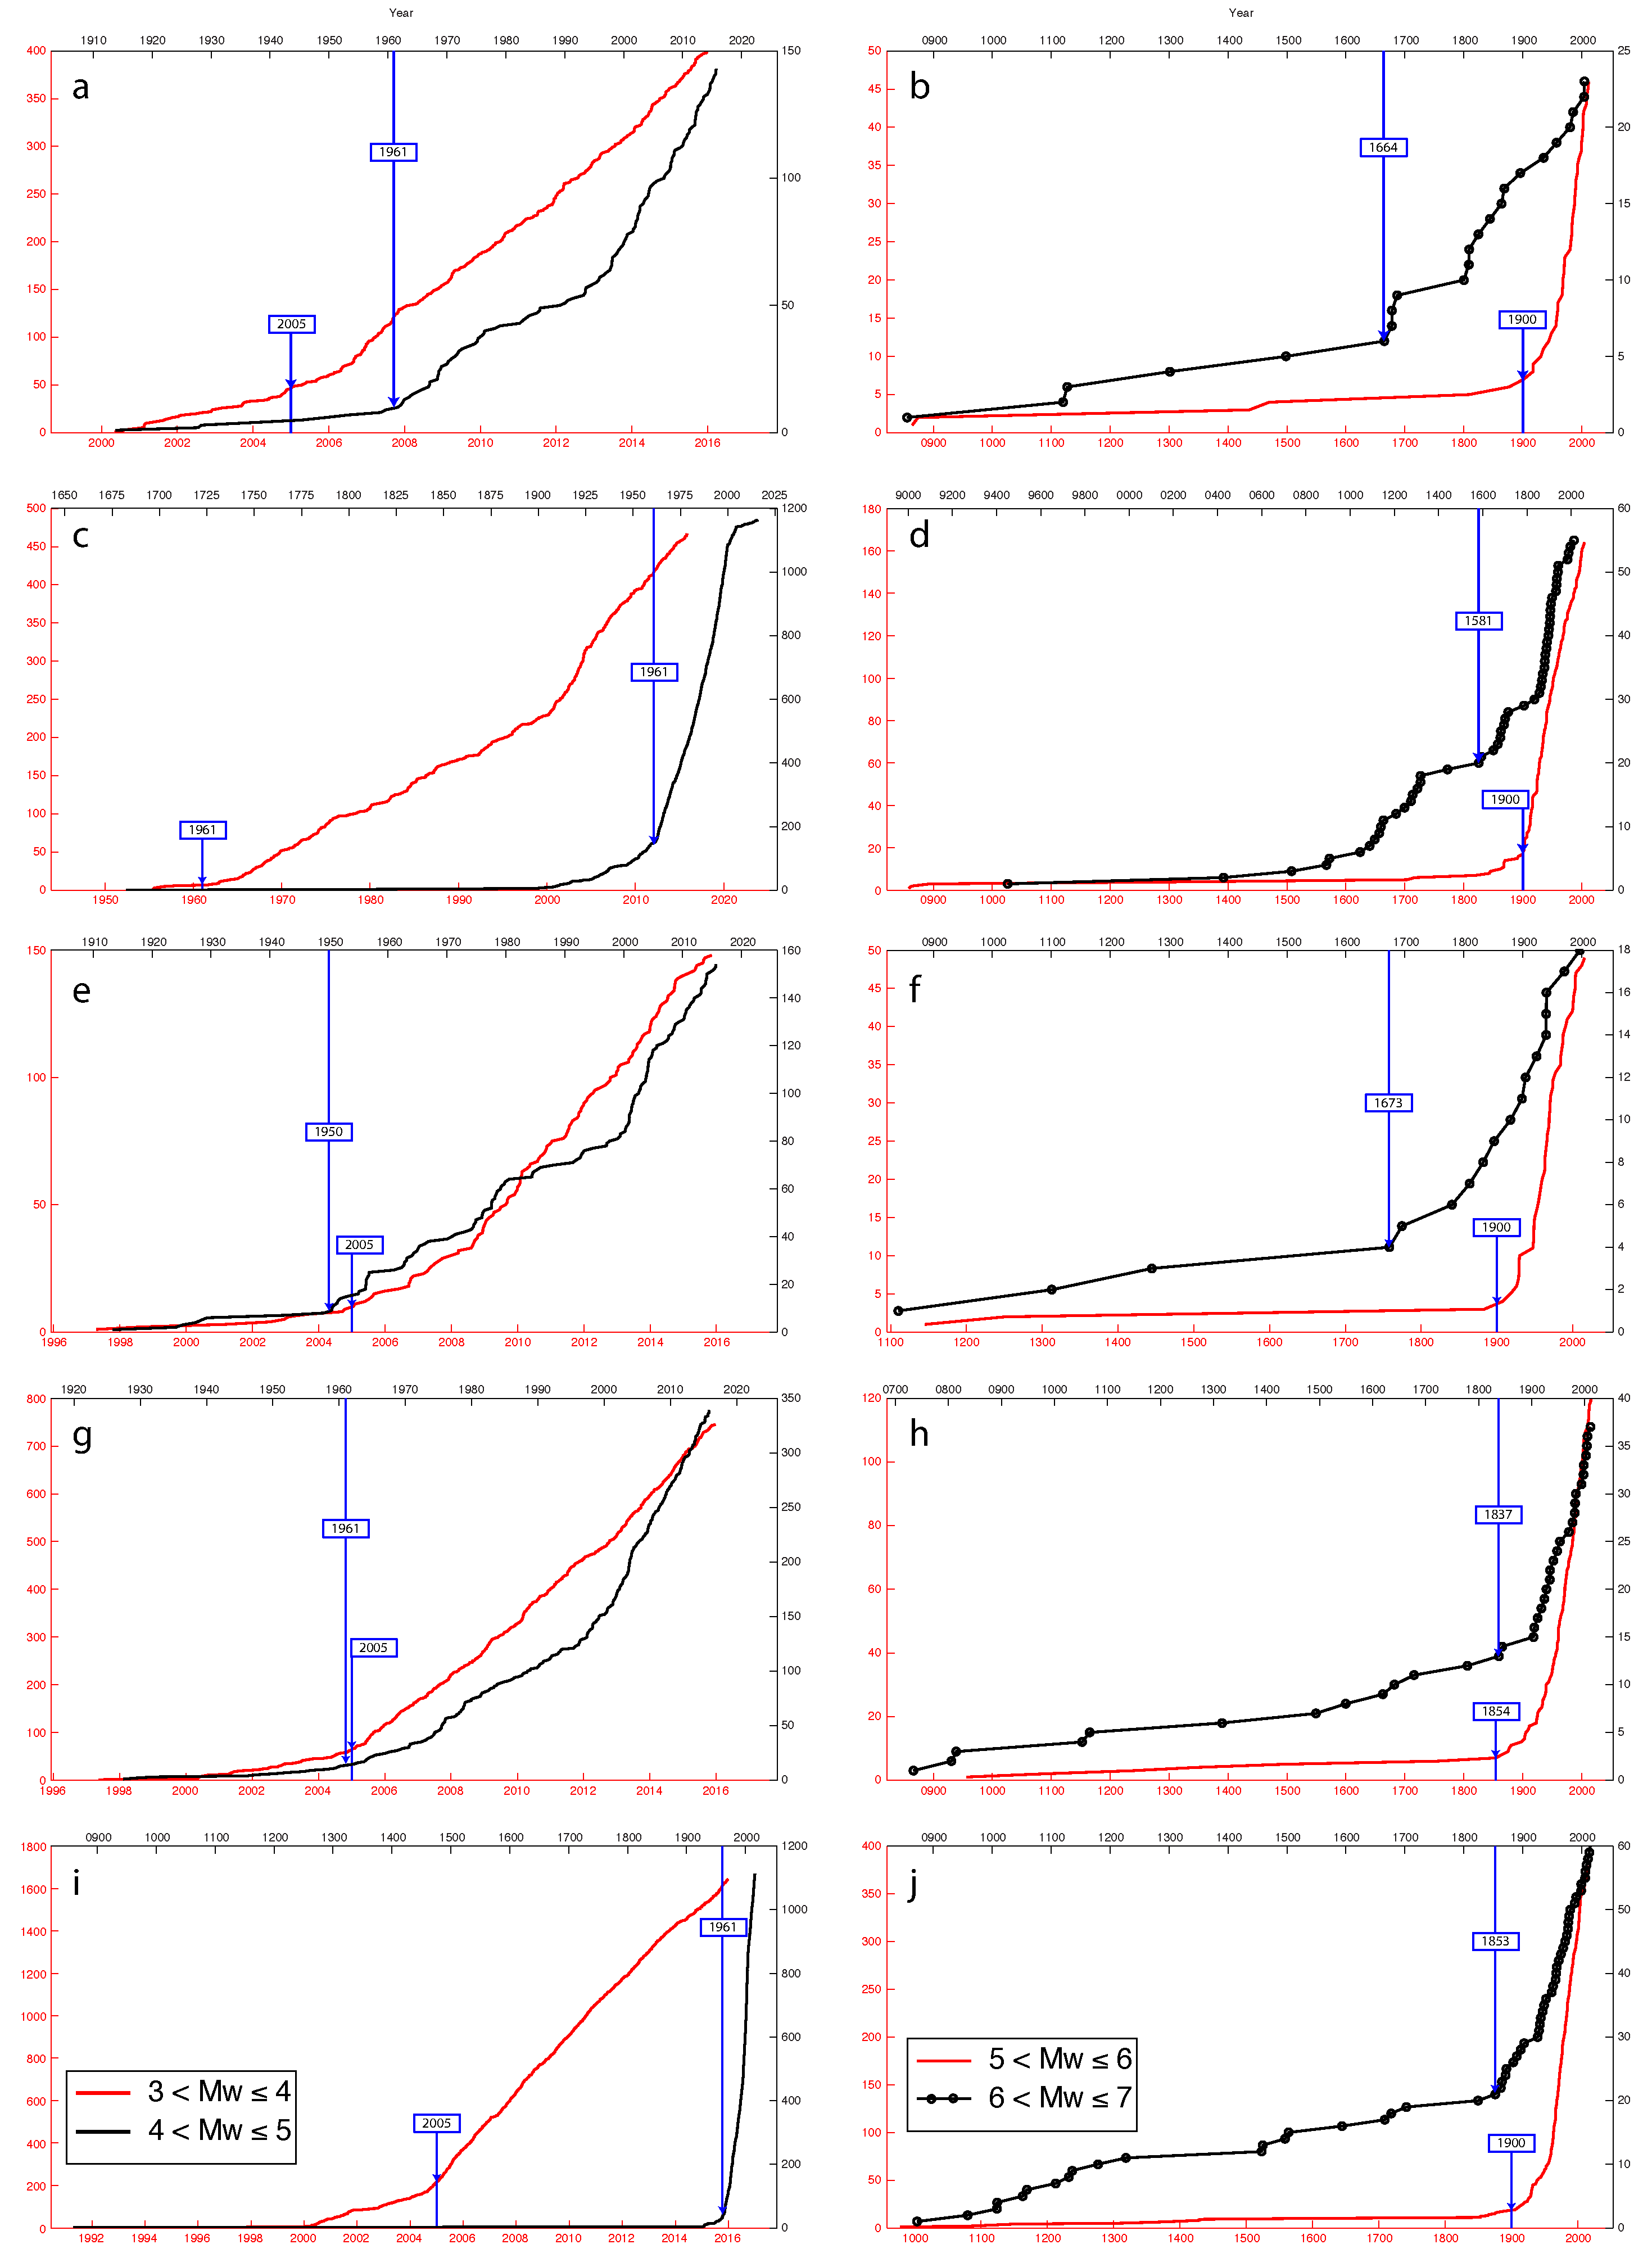
\includegraphics[scale=0.28]{figures/pdf/comp_test_all_mag.pdf} 
%\caption{Magnitude-time distribution of earthquakes in the study regions. a-b) Alborz, c-d) Azerbaijan, e-f)Kopek Dagh, g-h)Kopeh Dagh, i-j)Zagros}
%\label{fig:comp_test_all_mag}
%\end{figure*}
%
%
%
%\begin{table*}[!ht]
%\centering
%\caption{Completeness threshold of tectonic seismic regions.}
%\begin{tabular}{ccccccccc}
% ~           & Azerbaijan & Alborz & Kopeh Dagh & Central Iran & Zagros & North Iran  \\ \hline
%3-4         & 1961          & 2005   & 2005             & 2005            & 2005    & 2005          \\ \hline
%4-5         & 1961          & 1961   & 1950             & 1961            & 1961    & 1961          \\ \hline
%5-6         & 1900          & 1900   & 1900             & 1854            & 1900    & 1900           \\ \hline
%6-7         & 1581          & 1664   & 1673             & 1837            & 1853    & 1778           \\ \hline
%7 $< $    & 1042          & -401    & 9                   & 762              & 1439    & -401            \\ 
%\end{tabular}
%\label{tab:completeness}
%\end{table*}


% \section{Hazard Analysis Results}

% The PGA hazard maps have been computed for a 10\% and 2\% exceedance probability in 50 years, corresponding to a return period of 475 and 2475 years, from gridded values of historical and instrumental seismic activity. These levels of exceedance are a standard practice in seismic designs \citep{BHRC2014}.

% As mentioned earlier we broader the study region by 0.5\textdegree{}-perimeter to avoid the unexpected effect of outer border seismicity as well as avoiding the artifcial decay effect that results from smoothing the seismicity along and near the edges of the region of interest. Also it provides more uniform surrounding of the study area\citep{Lapajne1997}.

% We calculated the $a-values$ for each cell and spatially smoothed over a grid of $0.1 \times 0.1$ in latitude and longitude. We assume magnitude increment as $\Delta_M = 0.1$. In this model, events are not assigned to specific faults and are assumed to be potential seismogenic sources, and are spatially gridded to cells.

% Different correlation distances have been used in different studies, which are generally dependent on the accuracy of the location of the recorded earthquakes. \citet{Frankel1995} and \citet{Boyd2008} assumed the correlation distance to be 50 $km$. \citet{Barani2007} used distance of 25 $km$ based on previous studies that suggested the correlation function of the Alps and Apennines in Italy. \citet{Foteva2006} used 10 and 15 km in a different model. Correlation distance is a very sensitive parameter in smoothed seismic hazard maps, and it is a factor of uncertainty in earthquake location.

% Regarding the important parameters in determining the location of earhtquake (e.g. velocity model, station distribution, number and quality of seismic phases),\citet{Mirzaei1997} believes the uncertainties of the most reliable epicenters are probably at least 10 km. In developing of seismic hazard zoning map for Iran,\citet{Zare2012} considered the epicentral uncertainty as 30 km. Even though the uncertainties are different for different events in terms of instrumental or historical events, in this study we assumed the correlation distance as 30 km because of the lack of knowledge about other historical events. 

Regarding the study domain and the 0.1 grid size, the total number of source as grid points is 13561. 

% Even though \citet{Kalkan2004} derived the attenuation relationship up to 250 km, since \citet{Zafarani2014} used data up to 200 km to evaluate the GMPEs, we set the model to compute the ground motions at distances of less than 200 km.

\subsection{Hazard Curve}

We calculated the probability of exceedance of the ground motion from different ground motion levels, separately for each of 5 regions. We add the probability of all regions in order to have the effect of seismicity from all tectonic seismic regions. The results are presented as annual rate of exceedance. Fig.~\ref{fig:hazardcurve} represents the hazard curve of different model for some of important northern cities in Iran. 

\begin{figure*} [!ht]
\centering
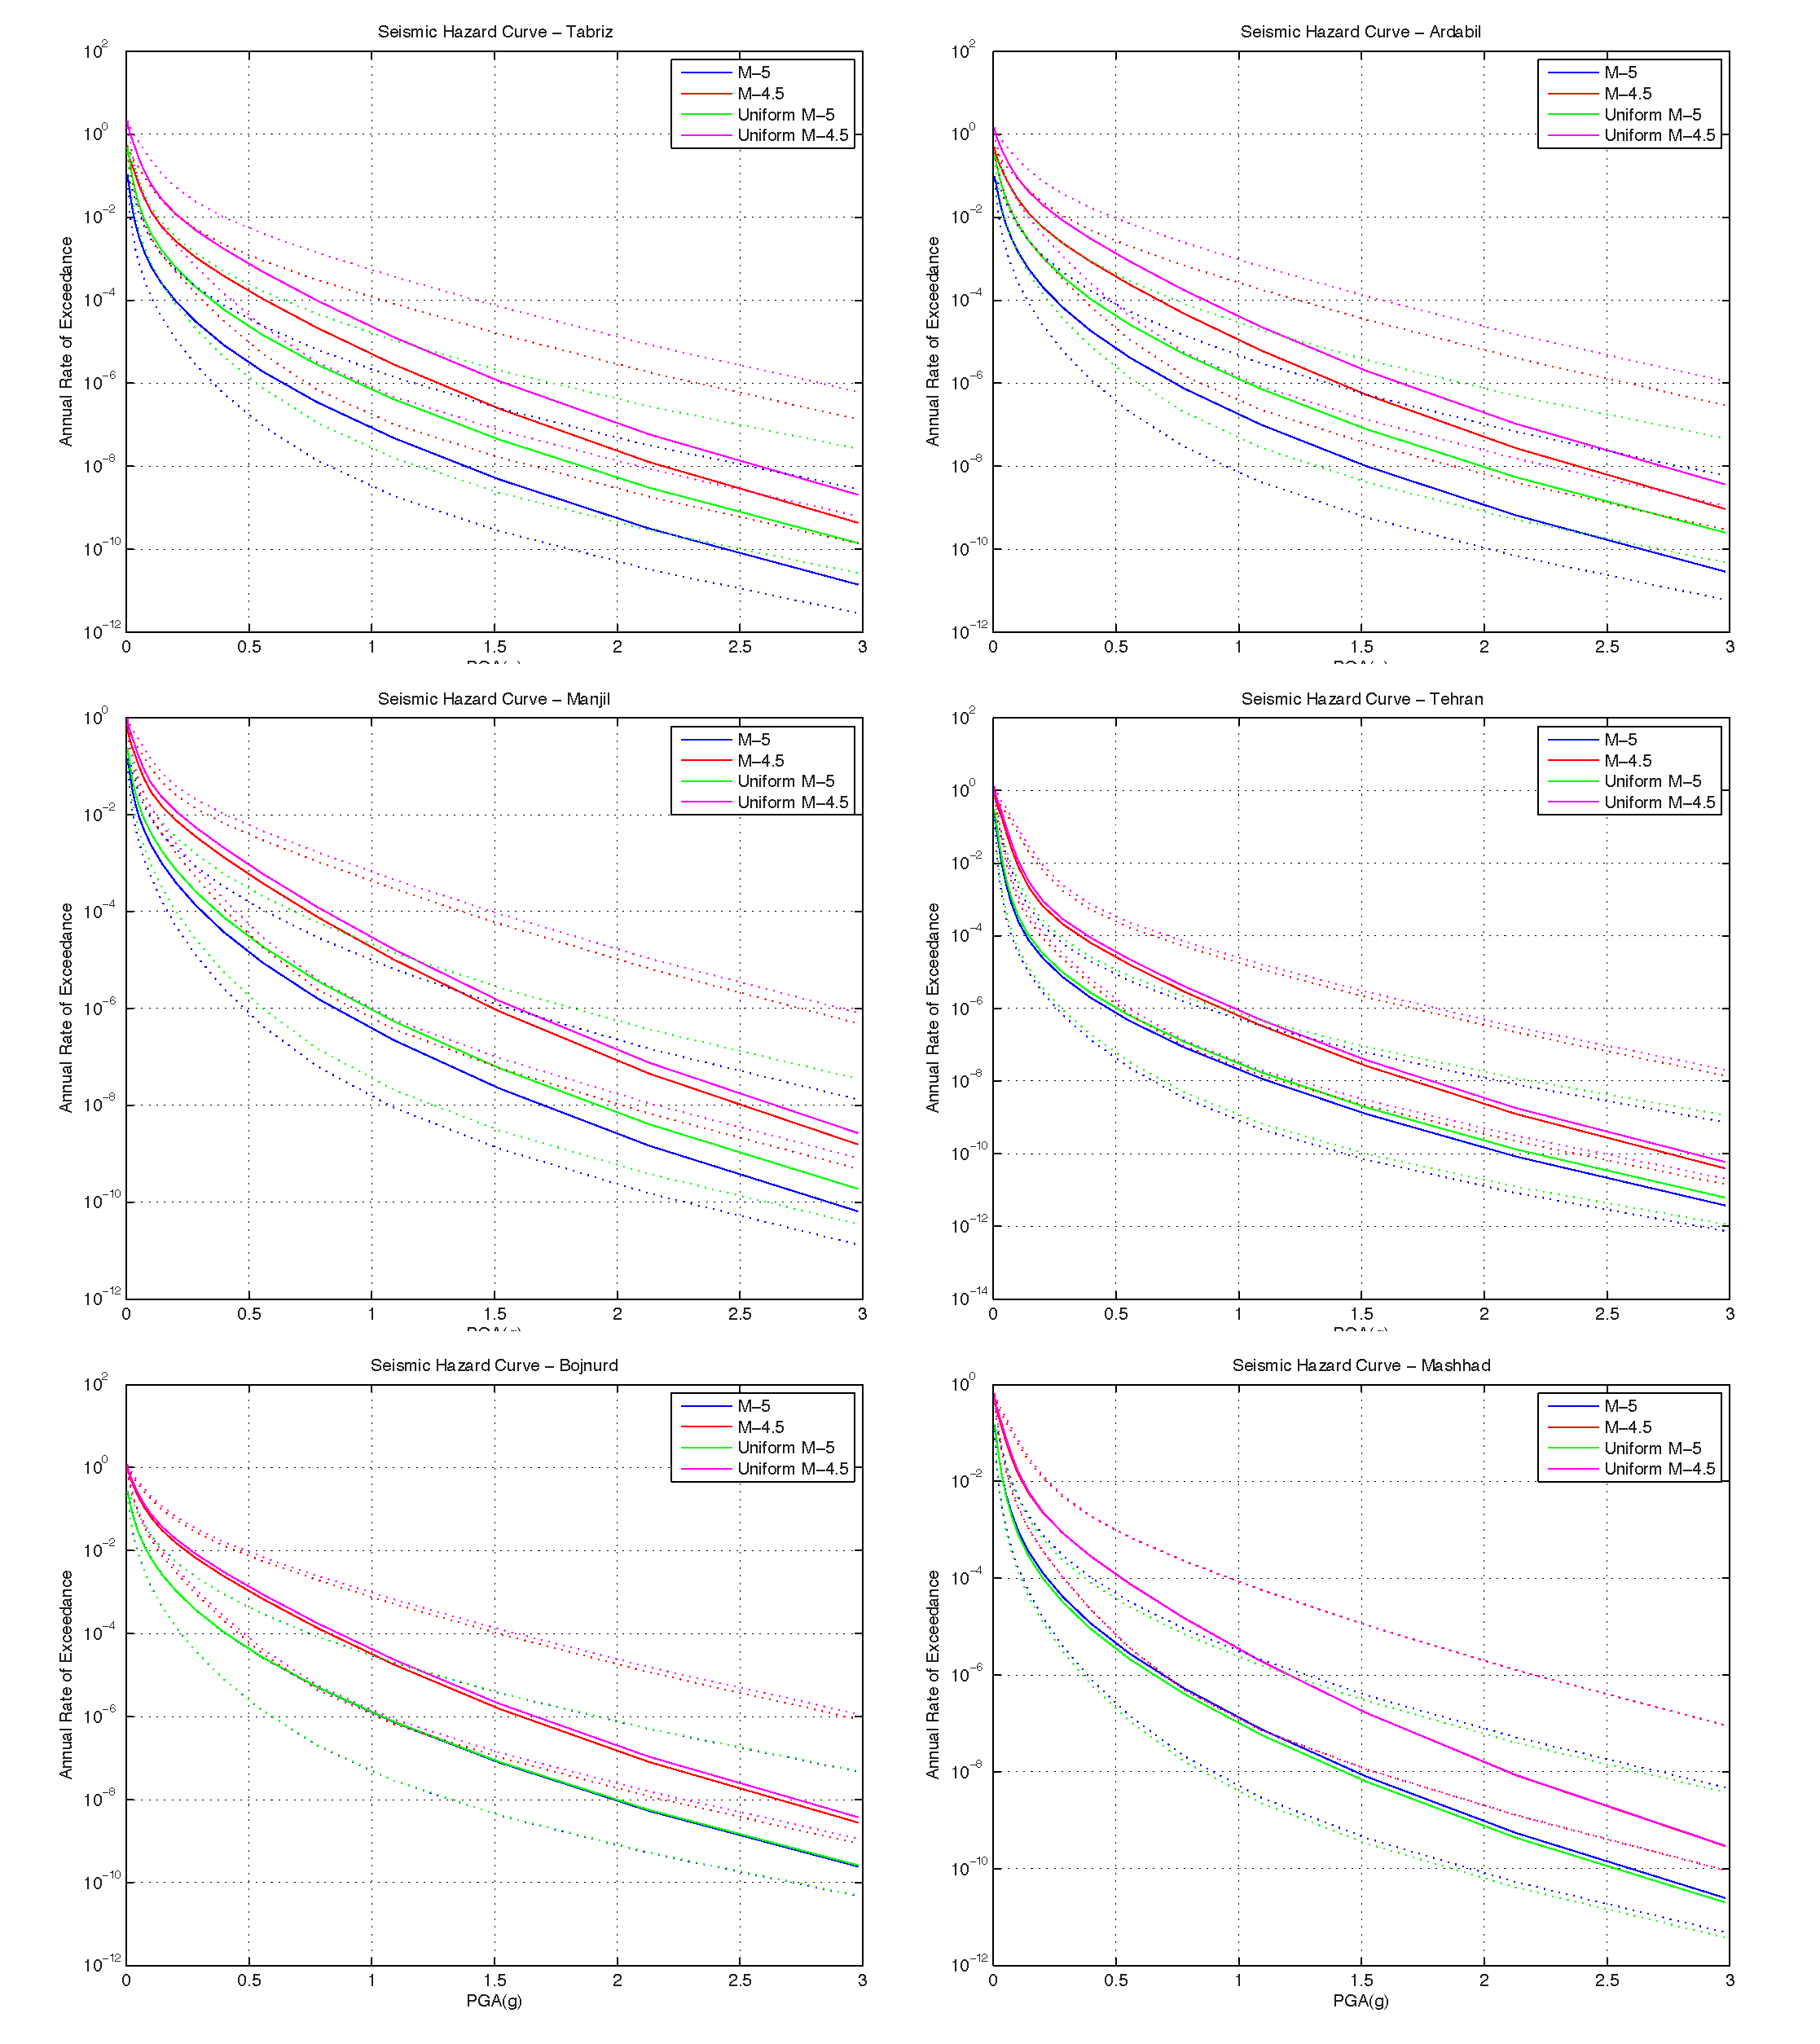
\includegraphics[scale=0.4]{figures/pdf/HazardCurve.pdf} 
\caption{Seismic Hazard Curve of Northern Cities in Iran}
\label{fig:hazardcurve}
\end{figure*}

\subsection{Peak Ground Acceleration}

We pick the peak ground acceleration for 10\% and 2\% probability of exceedance in 50 years which correspond with 0.002 and 0.0004 annual rate of exceedance. Fig.~\ref{fig:pga_10_mean} and Fig.~\ref{fig:pga_2_mean} show the results for 10\% and 2\% probability of exceedance in 50 years, respectively. These results are according to the mean value of the attenuation relationship.

\begin{figure*} [!ht]
\centering
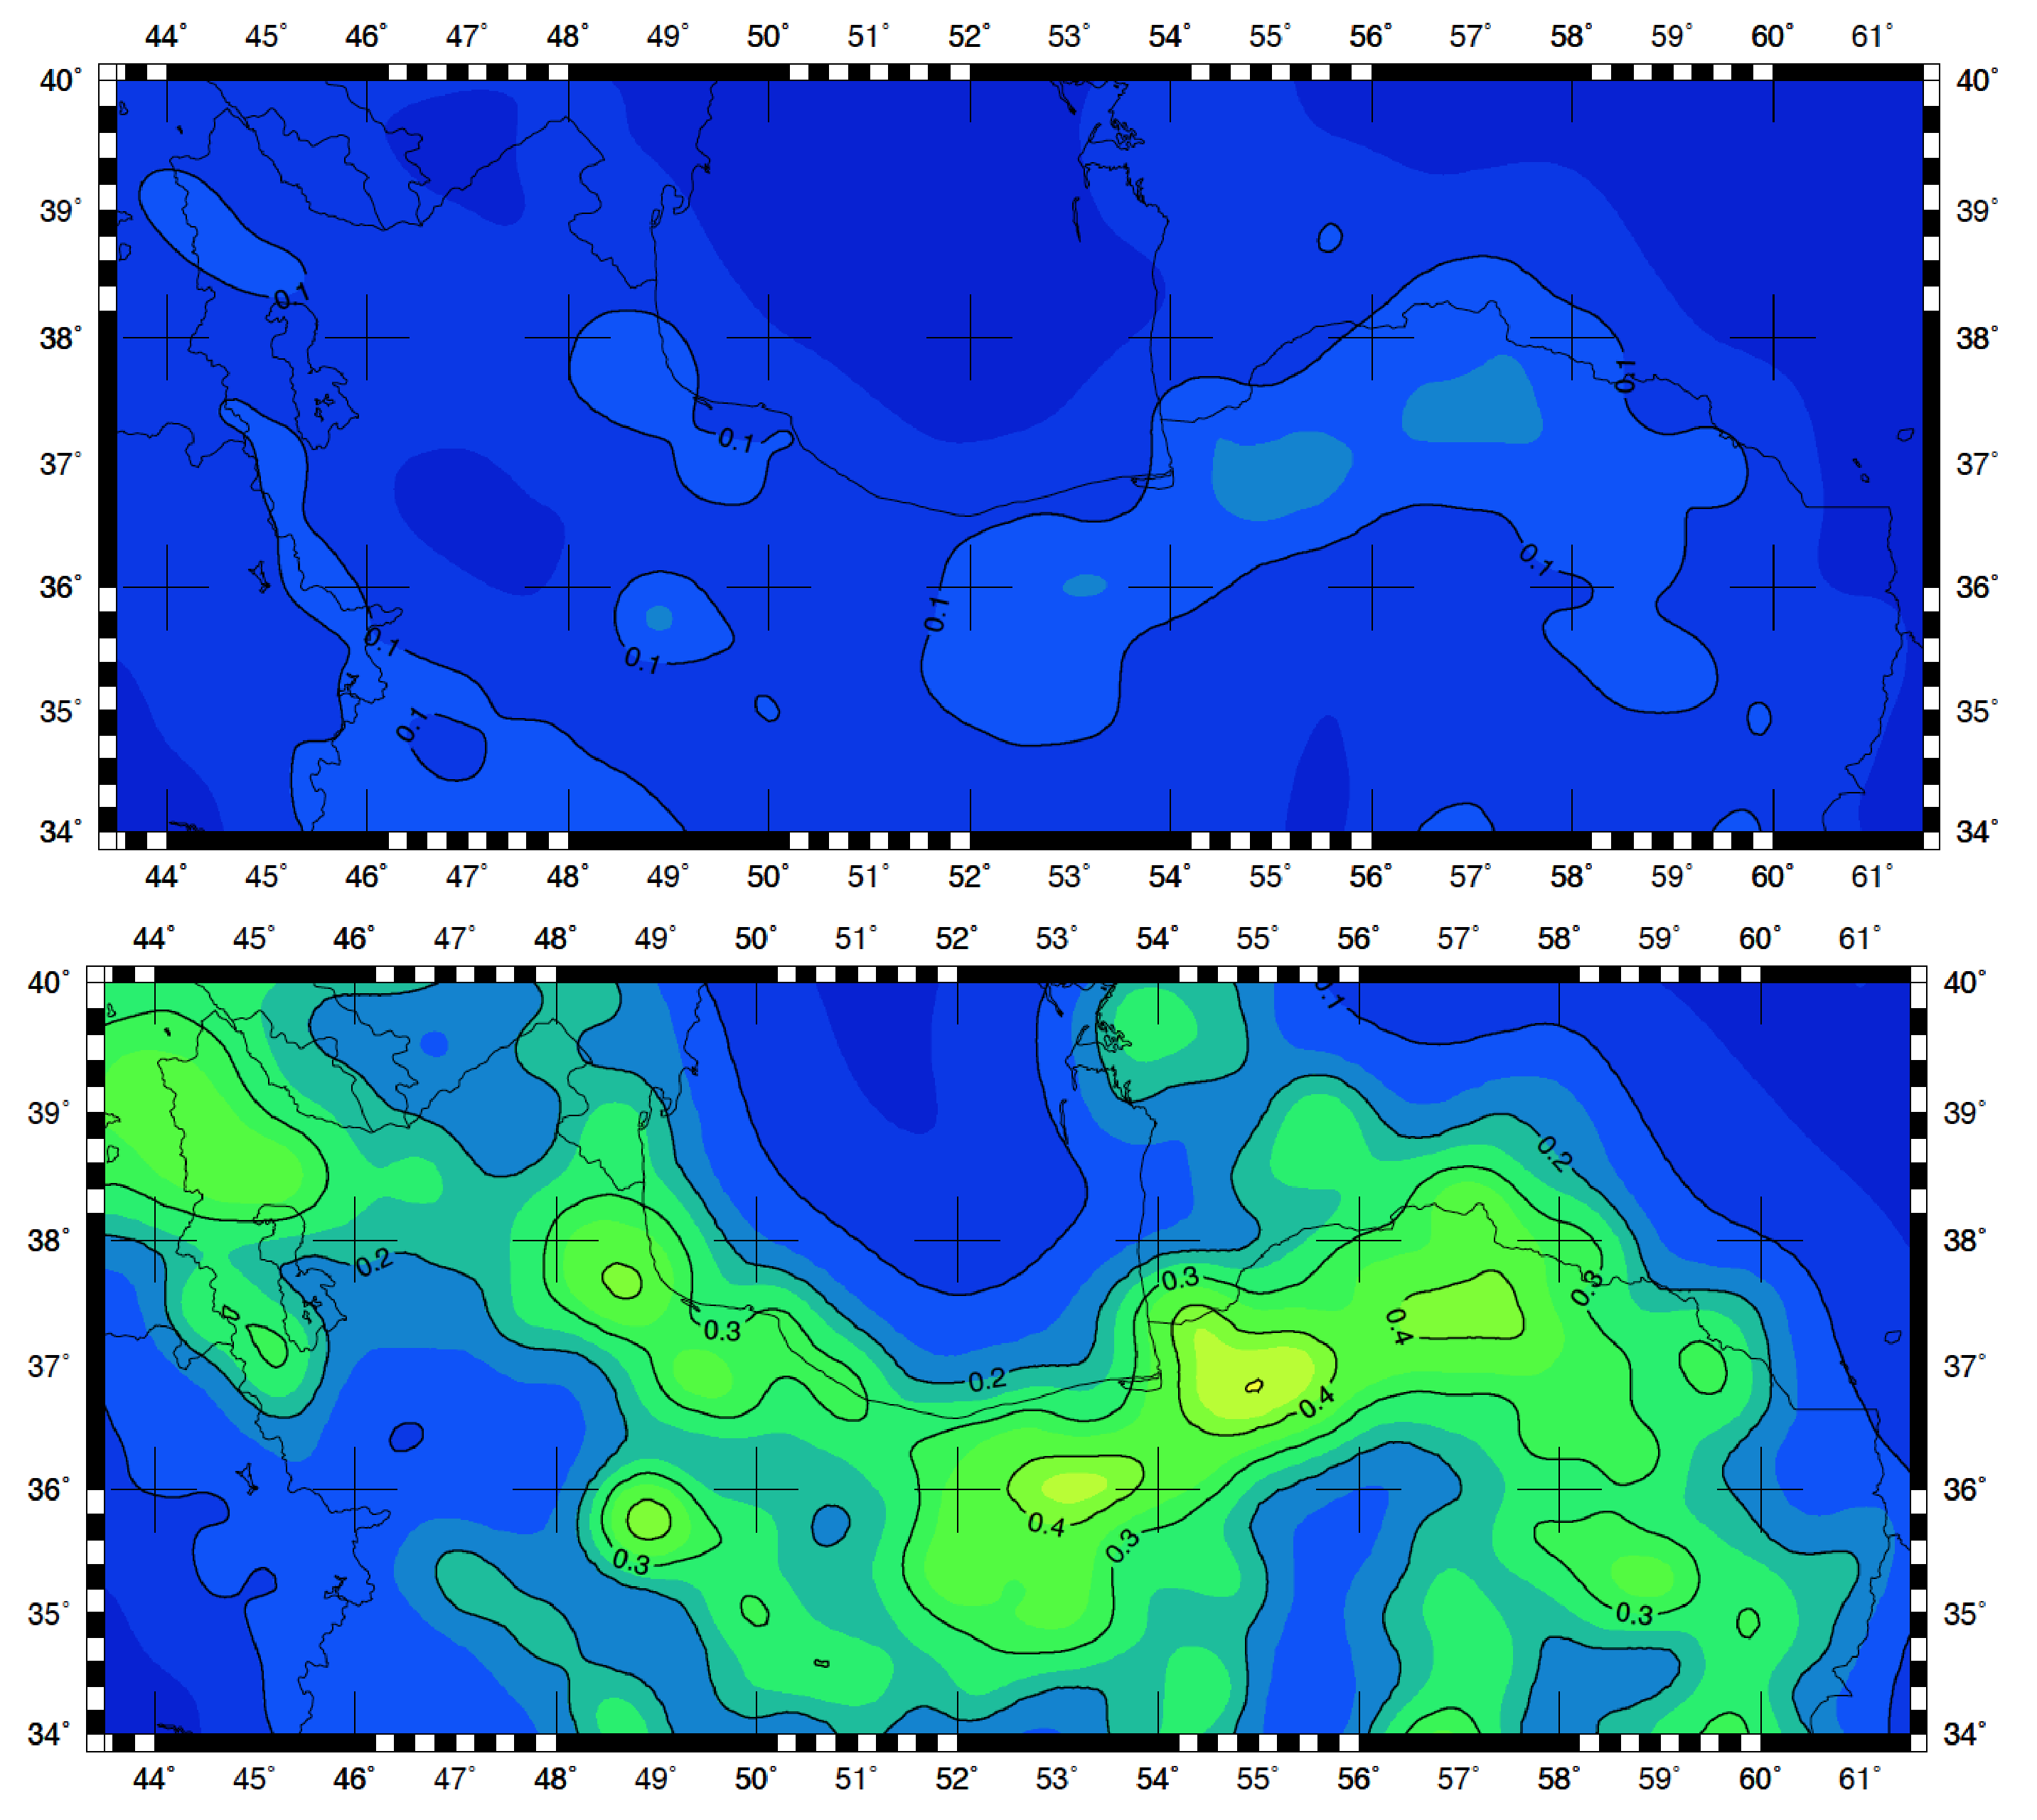
\includegraphics[scale=0.3]{figures/pdf/pga_10_mean.pdf} 
\caption{Peak ground acceleration for 10\% probability of exceedance in 50 years.}
\label{fig:pga_10_mean}
\end{figure*}

\begin{figure*} [!ht]
\centering
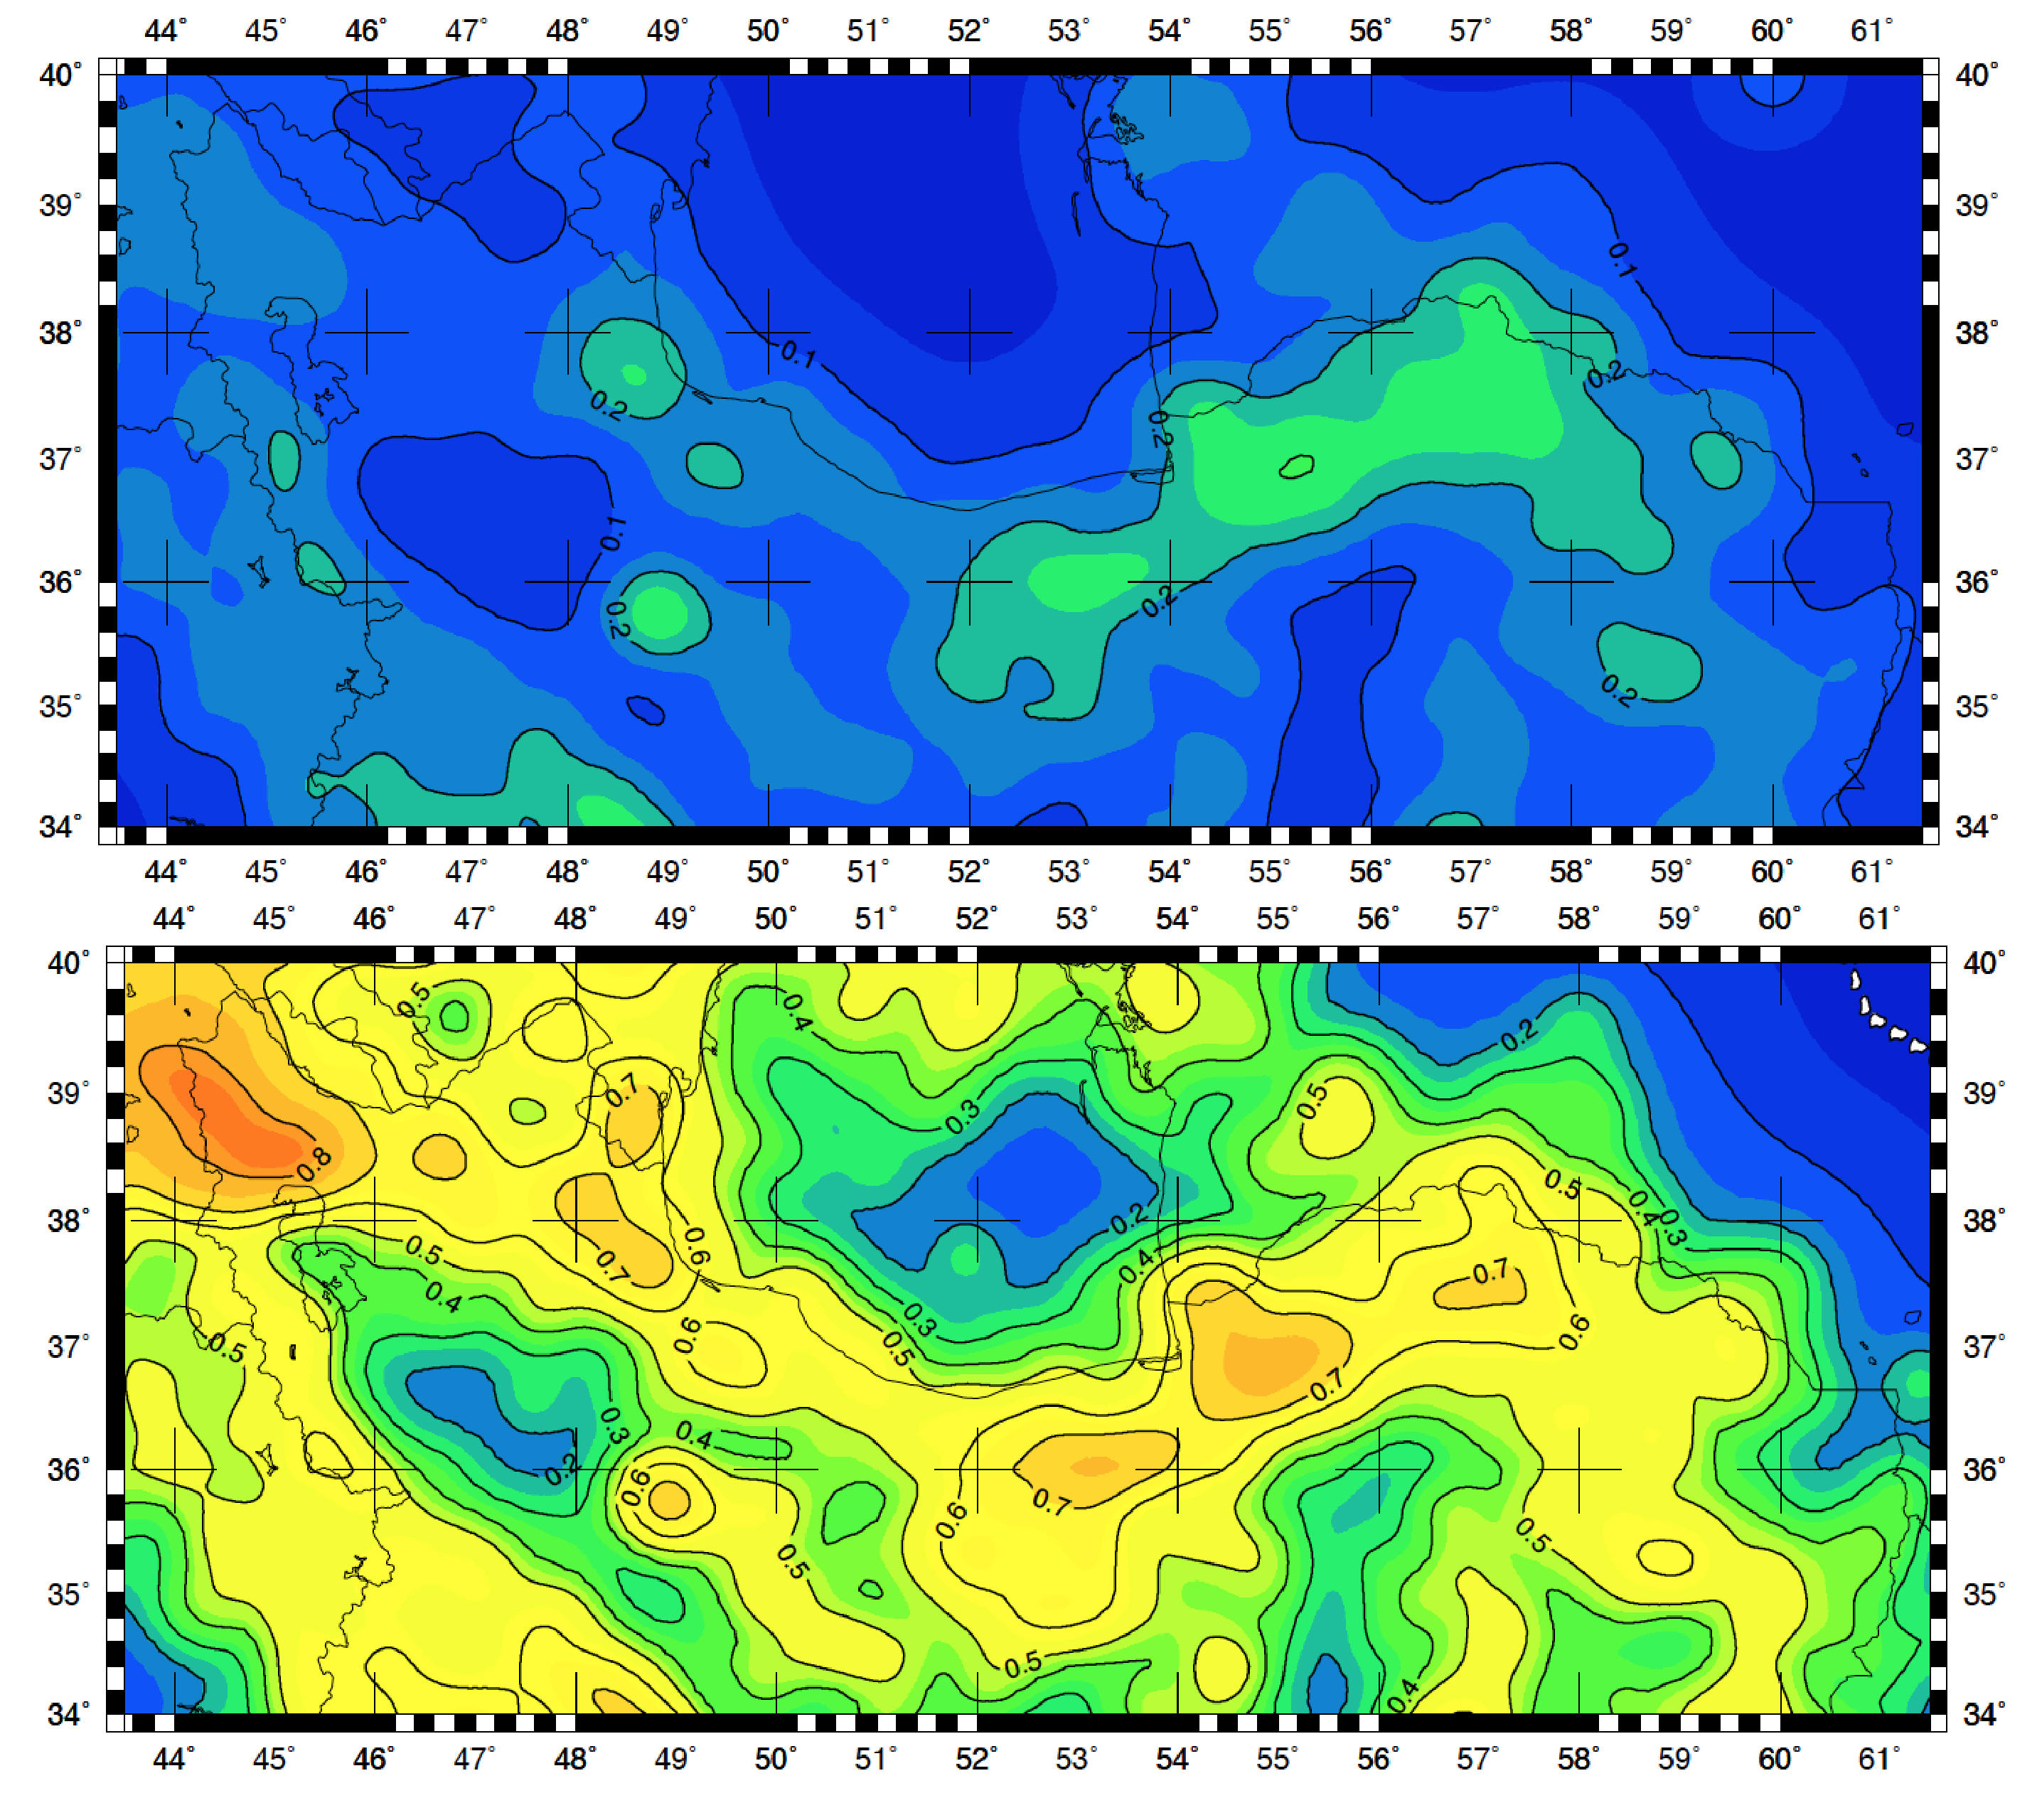
\includegraphics[scale=0.3]{figures/pdf/pga_2_mean.pdf} 
\caption{Peak ground acceleration for 2\% probability of exceedance in 50 years.}
\label{fig:pga_2_mean}
\end{figure*}

Fig.~\ref{fig:pga_10_mean_uniform} and Fig.~\ref{fig:pga_2_mean_uniform} show the results for 10\% and 2\% probability of exceedance in 50 years for the uniform model, respectively.

\begin{figure*} [!ht]
\centering
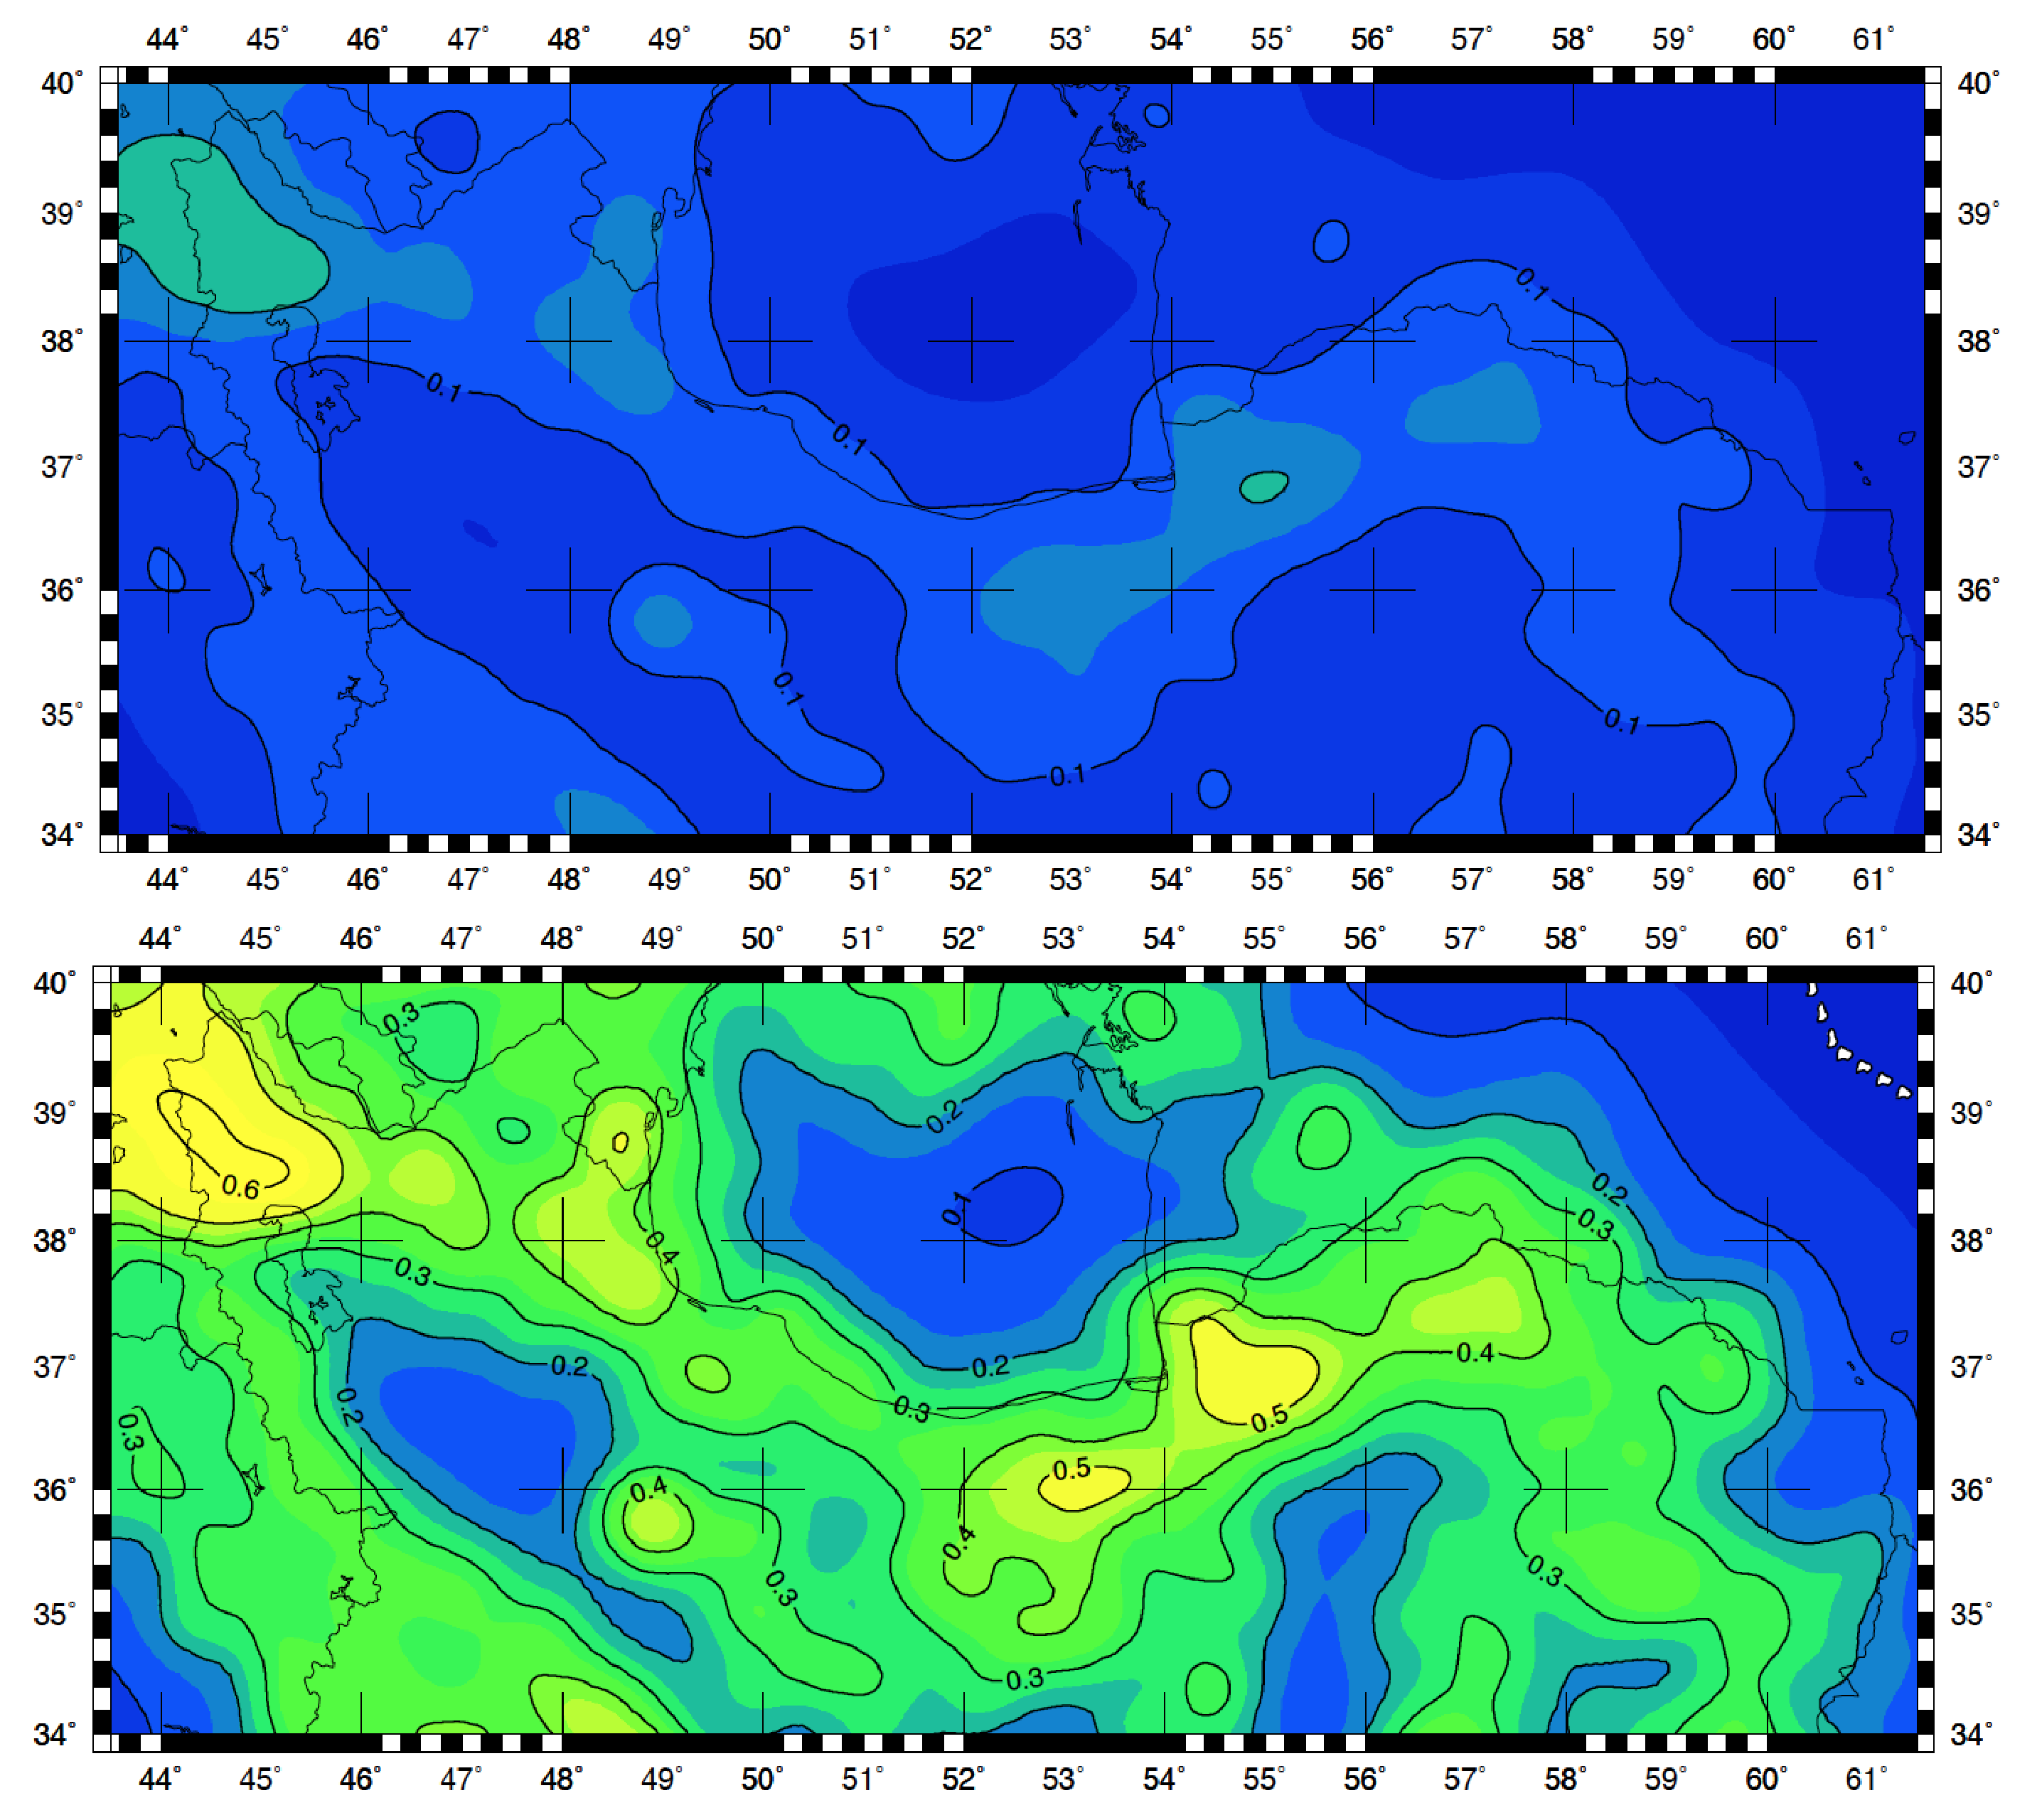
\includegraphics[scale=0.3]{figures/pdf/pga_10_mean_uniform.pdf} 
\caption{Peak ground acceleration for 10\% probability of exceedance in 50 years (uniform model).}
\label{fig:pga_10_mean_uniform}
\end{figure*}

\begin{figure*} [!ht]
\centering
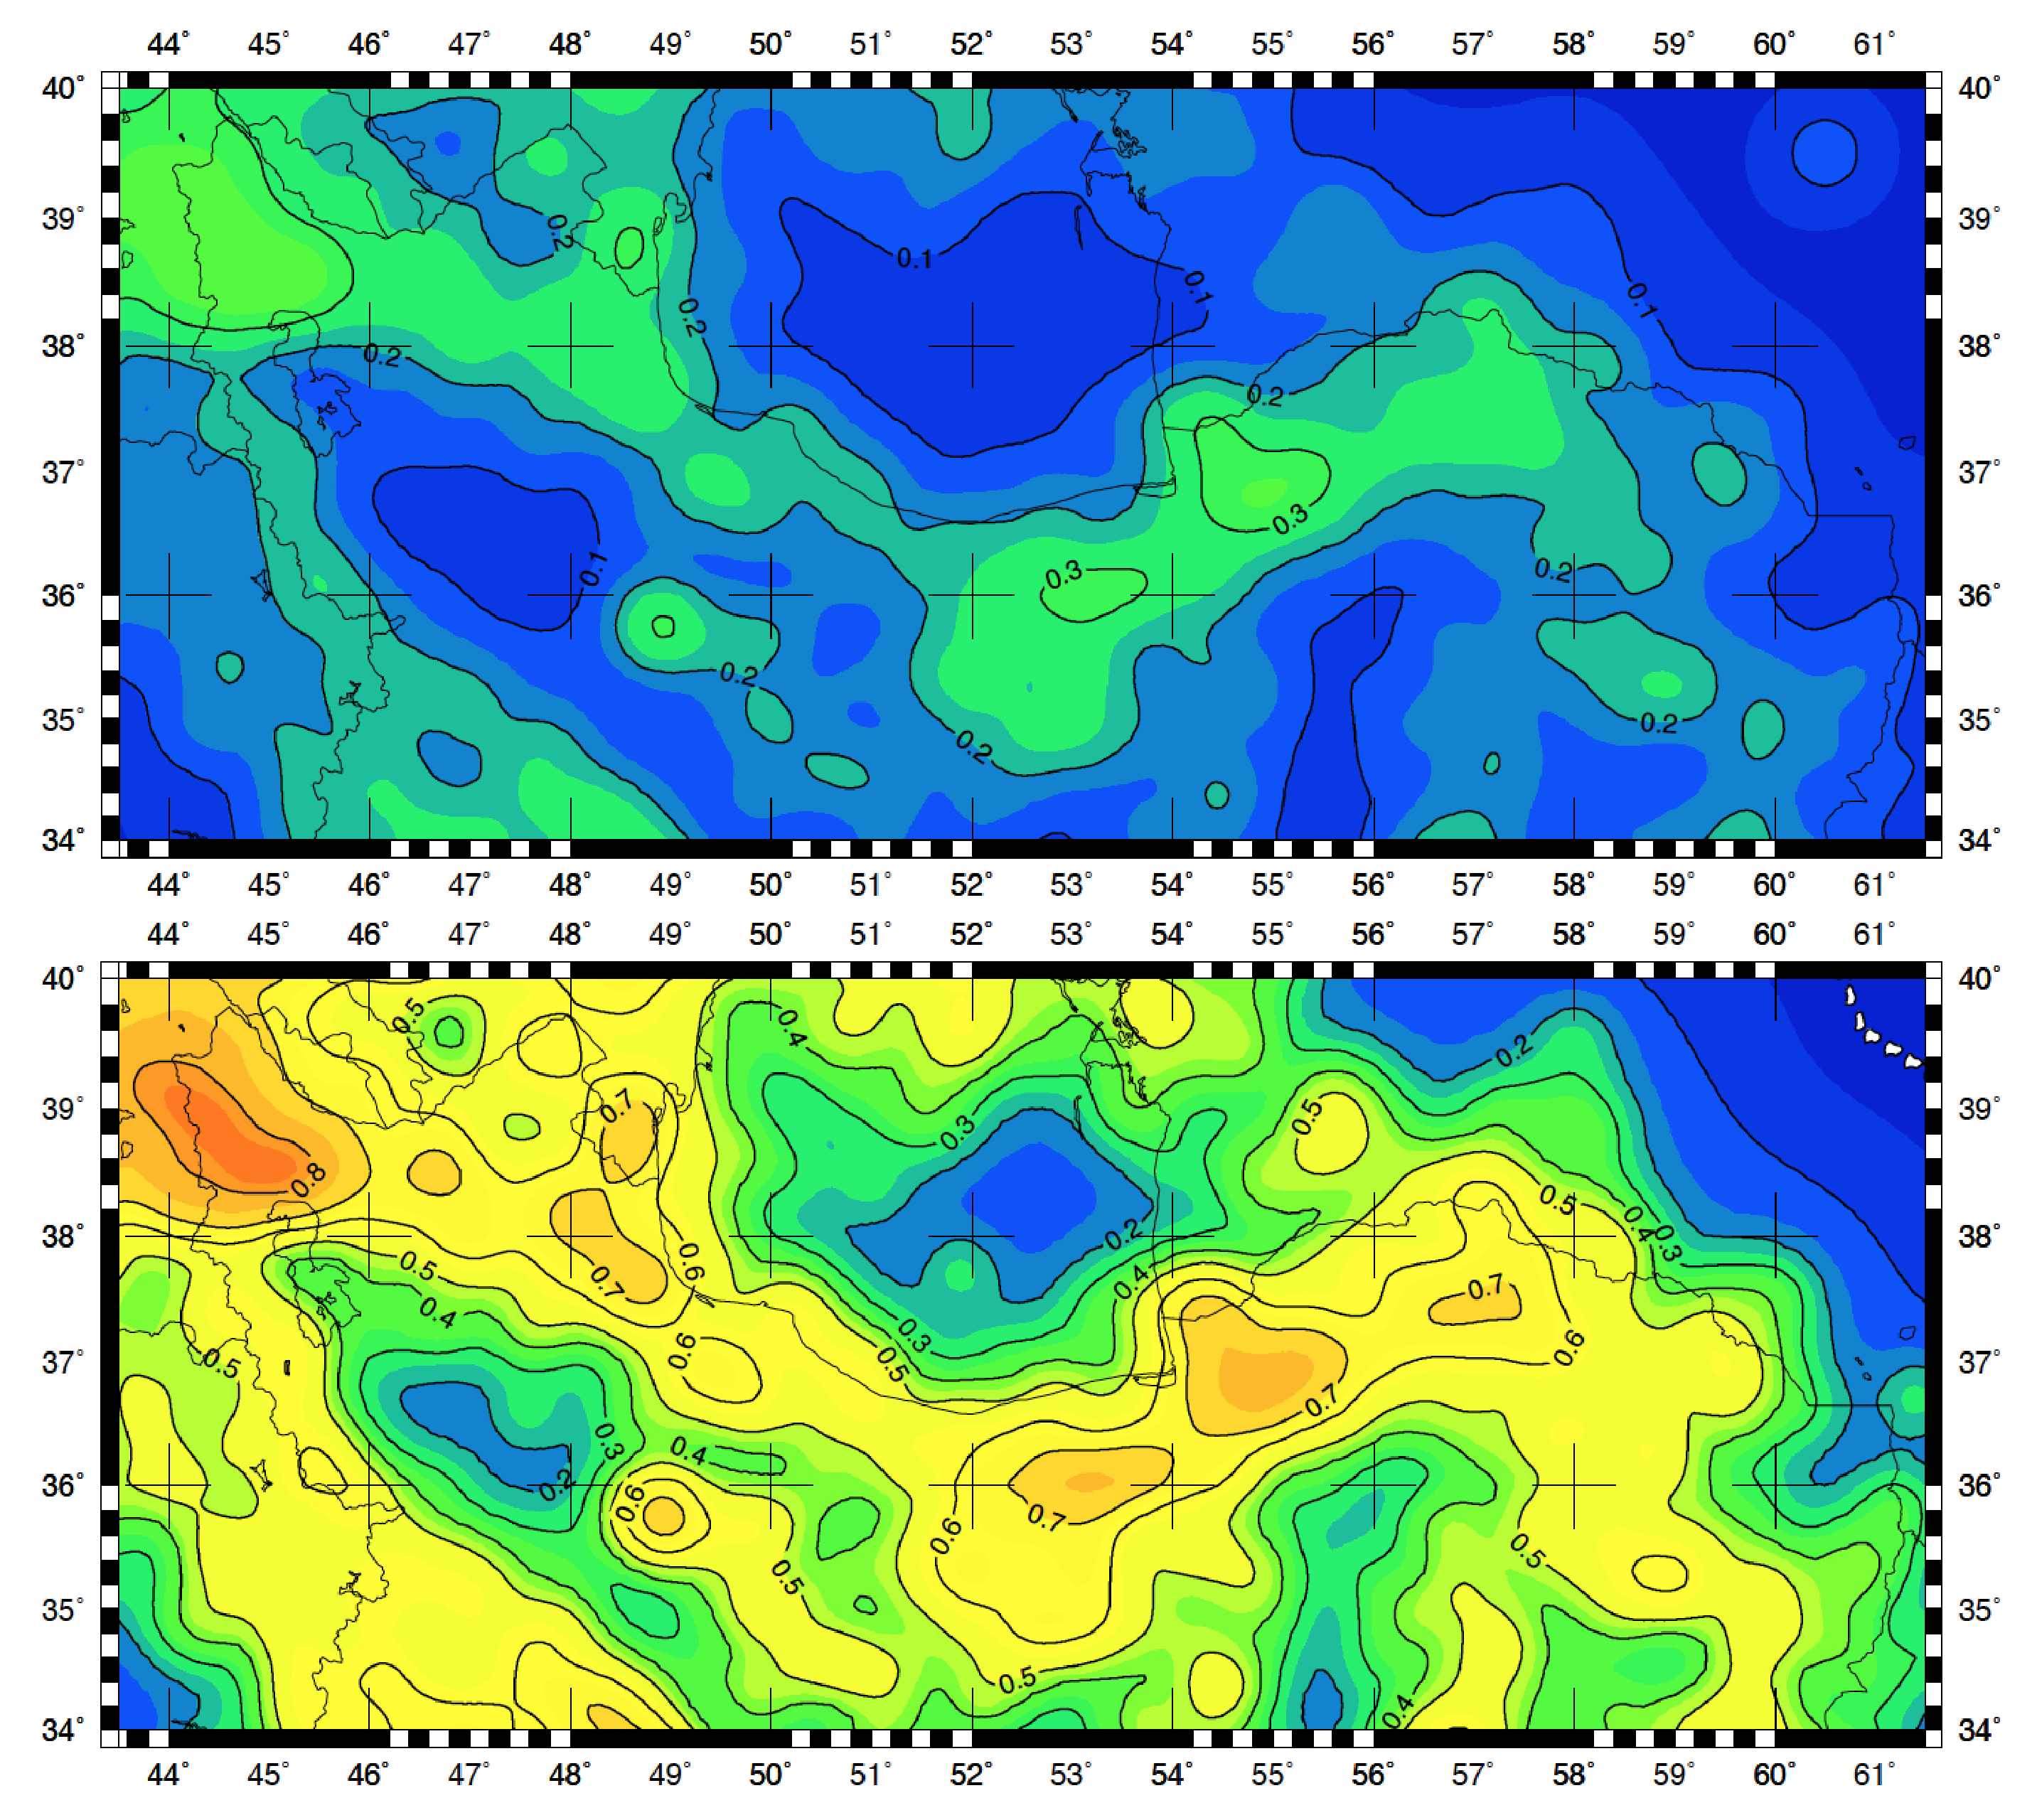
\includegraphics[scale=0.3]{figures/pdf/pga_2_mean_uniform.pdf} 
\caption{Peak ground acceleration for 2\% probability of exceedance in 50 years (uniform model).}
\label{fig:pga_2_mean_uniform}
\end{figure*}


% 
\section{Discussion of Results}

% Seismic hazard in northern Iran is computed based on background seismicity and projected on a set of hazard maps. The results obtained are represented as maps for the spatial distribution of horizontal peak ground acceleration with 10\% and 2\% probability of exceedance in 50 years, which correspond to the return period of 475 and 2475 years. 

The areas of large probabilistic ground motions clearly coincide with zones with a large number of events of magnitude 3.0 and larger. In this study we used two models for seismic hazard calculation, including $M_w>5$ and $M_w>4.5$. $M_w$ is the minimum magnitude that can affect the engineering site. 

In the probabilistic seismic hazard analysis increasing minimum magnitude will decrease the mean rate of earthquake occurrence ($\nu=exp(\alpha - \beta M_0)$), and also increase the value for the probability density function in the initial magnitudes. In a simple source the difference between different models specially in higher pga levels is negligible. However, in this study where we consider each event as a seismic source with different $\alpha$ and $\beta$ value, the results are considerably different. According to our results the reduction of the mean rate of earthquake occurrence has considerable effect on the results. 

% Results are presented for different models. In general in the models based on combination of five tectonic seismic regions there are five regions with high pga values. These regions are including: 40 km East of Gorgan (54.9,36.8), 50 km NW of Semnan(53.1,36), 110 km SW of Qazvin(48.9,35.8), 70 km SE of Ardabil(48.7,37.7), and 105 km North of Urmia(45.1,38.5). The pga values for each model at the mentioned places is presented in Table ~\ref{tab:pga_values_models}


% \begin{table*}[!ht]
% \centering
% \caption{ Regions with higher Pga values (in g) for 5-regions model. }
% \begin{tabular}{ cccccccccccccc}
% 	& & \multicolumn{6}{c}{10\% probability of exceedance in 50 years} & \multicolumn{6}{c}{2\% probability of exceedance in 50 years}    \\ 
% 	\cline{3-14}   & & \multicolumn{3}{c}{ $M_w > 5$ } & \multicolumn{3}{c}{ $M_w > 4.5$} & \multicolumn{3}{c}{ $M_w > 5$ } & \multicolumn{3}{c}{ $M_w > 4.5$ } \\ 
% 	\cline{3-14}    Lon & Lat & $-\sigma $ & $Mean$ & $+\sigma$ & $-\sigma $& $Mean$ &$+\sigma$& $-\sigma $ & $Mean$ & $+\sigma$& $-\sigma $ & $Mean$ & $+\sigma$ \\ \hline
% 	54.9	&	36.8	&	0.10	&	0.18	&	0.32	&	0.27	&	0.50	&	0.92	&	0.16	&	0.29	&	0.54	&	0.39	&	0.73	&	1.37 \\ \hline
% 	53.1	&	36.0 	&	0.09	&	0.16	&	0.28	&	0.26	&	0.47	&	0.85	&	0.14	&	0.27	&	0.51	&	0.38	&	0.71	&	1.31 \\ \hline
% 	48.9	&	35.8	&	0.09	&	0.16	&	0.28	&	0.24	&	0.44	&	0.79	&	0.15	&	0.28	&	0.52	&	0.37	&	0.68	&	1.24 \\ \hline
% 	48.7	&	37.7	&	0.07	&	0.14	&	0.26	&	0.23	&	0.42	&	0.76	&	0.14	&	0.25	&	0.46	&	0.36	&	0.66	&	1.20 \\ \hline
% 	45.1	&	38.5	&	0.06	&	0.11	&	0.20	&	0.20	&	0.38	&	0.72	&	0.11	&	0.20	&	0.38	&	0.34	&	0.61	&	1.08 \\ \hline
% \end{tabular}
% \label{tab:pga_values_models}
% \end{table*}

Using different approaches, probabilistic seismic hazard analyses have been conducted for the northern Iran. \citet{Tavakoli1999}, based on probabilisitic seismic computation using the historical and instrumental earthquake data, geology, tectonics, fault activity and seismic source model in Iran, prepared a new seismic hazard map of Iran. They divided Iran into 20 seismic tectonic regions and used seismic data up to 1997. They used \citet{Kijko1992} method  to determine the seismicity parameters. The results were displayed for the return period of 75 and 475 years. They predicted the maximum mean acceleration, near north Tabriz fault zone, North Tehran fault zone, and Dasht-e-Bayaz fault zone, to be around 0.45g for return period of 475 years. The smallest value of 0.35g for 475 years is predicted in a narrow band trending NW-SE and extending from Urmia to Isfahan.  

Using logic tree approach,\citet{Ghodrati2003} predicted the peak ground acceleration for Tehran for 475 years of return period. They used historical and instrumental data inside a circle of 200 km around the Tehran and converted them into $M_s$ magnitude scale. They used maximum likelihood method to get the seismicity parameters. Their results represented the peak ground acceleration for 10\% probability of exceedance in 50 years to be in range of $0.27g - 0.46g$.

\citet{Ghodrati2008} studied seismic hazard and seismic zoning of Gilan province based on probabilistic approach. They used 3 attenuation relationship and 2 seismicity parameters through logic three approach. They presented the map of the maximum probable acceleration over bedrock for 475 and 2475 year return periods. The pga in the interested area, ranges from 0.1g to 0.3g and 0.2g to 0.45g for 475 and 2475 year return periods, respectively. 

\citet{Vafaie2011} compiled a seismic catalog from 8th century A.D to 2006 for considering the near field effect earthquake PGA in Tabriz city in north-west of Iran. They used two attenuation relationships. They predicted the PGA for 475 and 2475 years of return period to be in range of 0.2 - 0.65 g and 0.3 - 0.9 g, respectively.  

Using linear source model,\citet{Rahgozar2012} conducted a probabilistic assessment of PGA and uniform hazard spectra for Bojnurd city, the Capital of North Khorasan Province, Iran. They found the seismicity parameters of historical and instrumental data through \citet{Kijko2000} approach. They predicted the peak ground acceleration for three different attenuation relationships through implementing in the SEISRISK III software \citep{Bender1982}, and combine the results through logic tree approach. The results indicate that the PGA for 475 and 2475 years of return period will be in range of 0.15-0.22 g and 0.28-0.49 g, respectively.

Using  EZ-FRISK computer program and considering $M_{min} = 4$ as a minimum magnitude that can affect the engineering site, \citet{Abdi2013} evaluated a probabilistic seismic hazard analysis for Tehran and surrounding areas in order to quantify the dominant events that have the most contribution on ground motion exceedance from different hazard level. They predicted the PGA for Tehran and Karaj city to be in range of 0.27 - 0.3 g for return period of 475 years. 

\citet{Abdollahzadeh2014a} carried out a probabilistic seismic hazard assessment for part of Northern Iran. They used the logic tree approach to capture the epistemic uncertainty of seismic hazard assessment in delineation of seismic sources and selection of attenuation relationship. They used three attenuation relationships and 2 seismic source models. They collected the earthquake catalog from various references and reported the pga for 475 and 2475 years of return period for northern cities.   

\citet{Golara2014} conducted a probabilistic seismic hazard analysis of interconnected infrastructure of Iranian high pressure gas supply system. He used line and area source model in order to estimate the Iranian  high-pressure gas supply system's ability to withstand a sudden large ground movements caused by potential earthquakes and related phenomenon that might be expected. he used simplified tectonic map after \citet{Alavi1991}. He used four attenuation relationships and presented the results for 2475 years of return period. 

\citet{Boostan2015} developed new model for probabilistic seismic hazard assessment based on fuzzy sets theory for Tehran, Iran. The results is about 0.42-0.48 g for 475 years. 

Table ~\ref{tab:pga_values} presents the PGA value for some of the major cities in northern Iran from different studies. This study values are results of 5-region model with $M_w > 4.5 $.

\begin{table*}[!ht]
\centering
\caption{Comparison of PGA, from different studies for selected cities in Northern Iran. This study values are results of 5-regions model with "$M_w > 4.5$" (V2011:  \citet{Vafaie2011}), G2008: \citet{Ghodrati2008}, B2015: \citet{Boostan2015},  G2003:  \citet{Ghodrati2003},  Az2014: \citet{Abdollahzadeh2014a} , Ra2012: \citet{Rahgozar2012} , Ab2013: \citet{Abdi2013} ) }
\begin{tabular}{ | c | c | c | c | c | c | c | c | c | c | c |}
\hline
	\multirow{2}{*}{Cities} & \multirow{2}{*}{Lon} & \multirow{2}{*}{Lat} & \multicolumn{2}{|c|}{This study} & \multirow{2}{*}{2800} & Zare & Golara &\multicolumn{3}{|c|}{Other Refrences}    \\ 
	\cline{4-5}  \cline{9-11}  &  &  & 10\% & 2\% &  &  2012 & 2014 & 10\% & 2\% & ref \\ \hline
	 Urumieh   & 45.1   & 37.6    & 0.25 & 0.41   & 0.3 & 0.35-0.5 & 0.3-0.5 &  &  &  \\ \hline
	 Tabriz       & 46.3    & 38.1   & 0.23 & 0.39   & 0.35 & 0.35-0.5 & 0.9-1.2& 0.2- 0.65 & 0.3 to 0.9 & V2011 \\ \hline
	 Ardabil      & 48.3   & 38.3   & 0.30 & 0.51    & 0.3 & 0.35-0.5 &0.5-0.7  &&  &  \\ \hline
	 Zanjan      & 48.5   & 36.7   & 0.19 & 0.32    & 0.3 & 0.35-0.5 &0.5-0.7  &&  &  \\ \hline
	 Manjil       & 49.4   & 36.7    & 0.33 & 0.53   & 0.35 & 0.65 $<$ &0.5-0.7& 0.25 & 0.4 & G2008 \\ \hline
	  \multirow{2}{*}{Rasht}  & \multirow{2}{*}{49.6} & \multirow{2}{*}{37.3} & \multirow{2}{*}{0.3} & \multirow{2}{*}{0.5} & \multirow{2}{*}{0.3} & \multirow{2}{*}{0.5-0.65} & \multirow{2}{*}{0.5-0.7} & 0.1 &  0.2 &  G2008 \\ 
	  \cline{9-11}	             &  &  &  &  &  &  & & 0.25-0.3 & 0.55-0.6 & Az2013\\ \hline
	 Qazvin     & 50.0   & 36.3    & 0.22 & 0.37   & 0.35 & 0.35-0.5 &0.5-0.7& 0.31 & 0.42 &  \\ \hline
	 Karaj        & 51.0   & 35.8    & 0.20 & 0.36   & 0.35 & 0.35-0.5 &0.7-0.9& 0.31 & 0.42 & Ab2013 \\ \hline
	 \multirow{3}{*}{Tehran}  & \multirow{3}{*}{51.4} & \multirow{3}{*}{35.7} & \multirow{3}{*}{0.27} & \multirow{3}{*}{0.45} & \multirow{3}{*}{0.35} & \multirow{3}{*}{0.35-0.5} & \multirow{3}{*}{0.7-0.9} & 0.37-0.42 &  &  G2003 \\ 
	 \cline{9-11}	             &  &  &  &  &  &  & & 0.27-0.3  &  & Ab2013\\ 
	 \cline{9-11}	             &  &  &  &  &  &  & & 0.42-0.48 &  & B2015\\ \hline
	 Sari          & 53.0   & 36.3   & 0.39   & 0.62  & 0.3 & 0.35-0.5 &0.5-0.7& 0.3 - 0.35 &  0.65 - 0.7 & Az2014\\ \hline
	 Semnan   & 53.4   & 35.6   & 0.36   & 0.55  & 0.3 & 0.35-0.5 &0.3-0.5&  & & \\ \hline
	 Gorgan    & 54.4   & 36.8    & 0.45  & 0.69  & 0.3 & 0.35-0.5 &0.5-0.7& 0.3 - 0.35 &  0.65 -0.7 & Az2014\\ \hline
	 Bojnurd   & 57.3    & 37.5    & 0.43  & 0.67  & 0.3 & 0.35-0.5 &0.7-0.9&0.16-0.2  & 0.32-0.45  & Ra2012  \\ \hline
	 Mashhad & 59.6     & 36.3   & 0.21 & 0.37  & 0.3 & 0.35-0.5 &0.7-0.9  &  &&  \\ \hline
\end{tabular}
\label{tab:pga_values}
\end{table*}

% \subsection{$\pm \sigma$ of attenuation relationship}

% In this study we use one attenuation relationship (See the discussion in the attenuation relationship section). In order to consider the uncertainty of the ground motion equation we also present the $\pm$ standard deviation of each seismic hazard model. These figures give an idea about the range of probable peak ground acceleration for 10\% and 2\% probability of exceedance in 50 years. Fig.~\ref{fig:pga_10_minus_plus} and Fig.~\ref{fig:pga_2_minus_plus} show the results of plus and minus standard deviation of attenuation relationship, respectively. 

% These figures show the variation of peak ground acceleration for each model. However, due to inability of the earth to carry more intense seismic waves, there is almost certainly some true physical upper bound on ground motion intensity \citep{Baker2008}


% \begin{figure*} [!ht]
% \centering
% 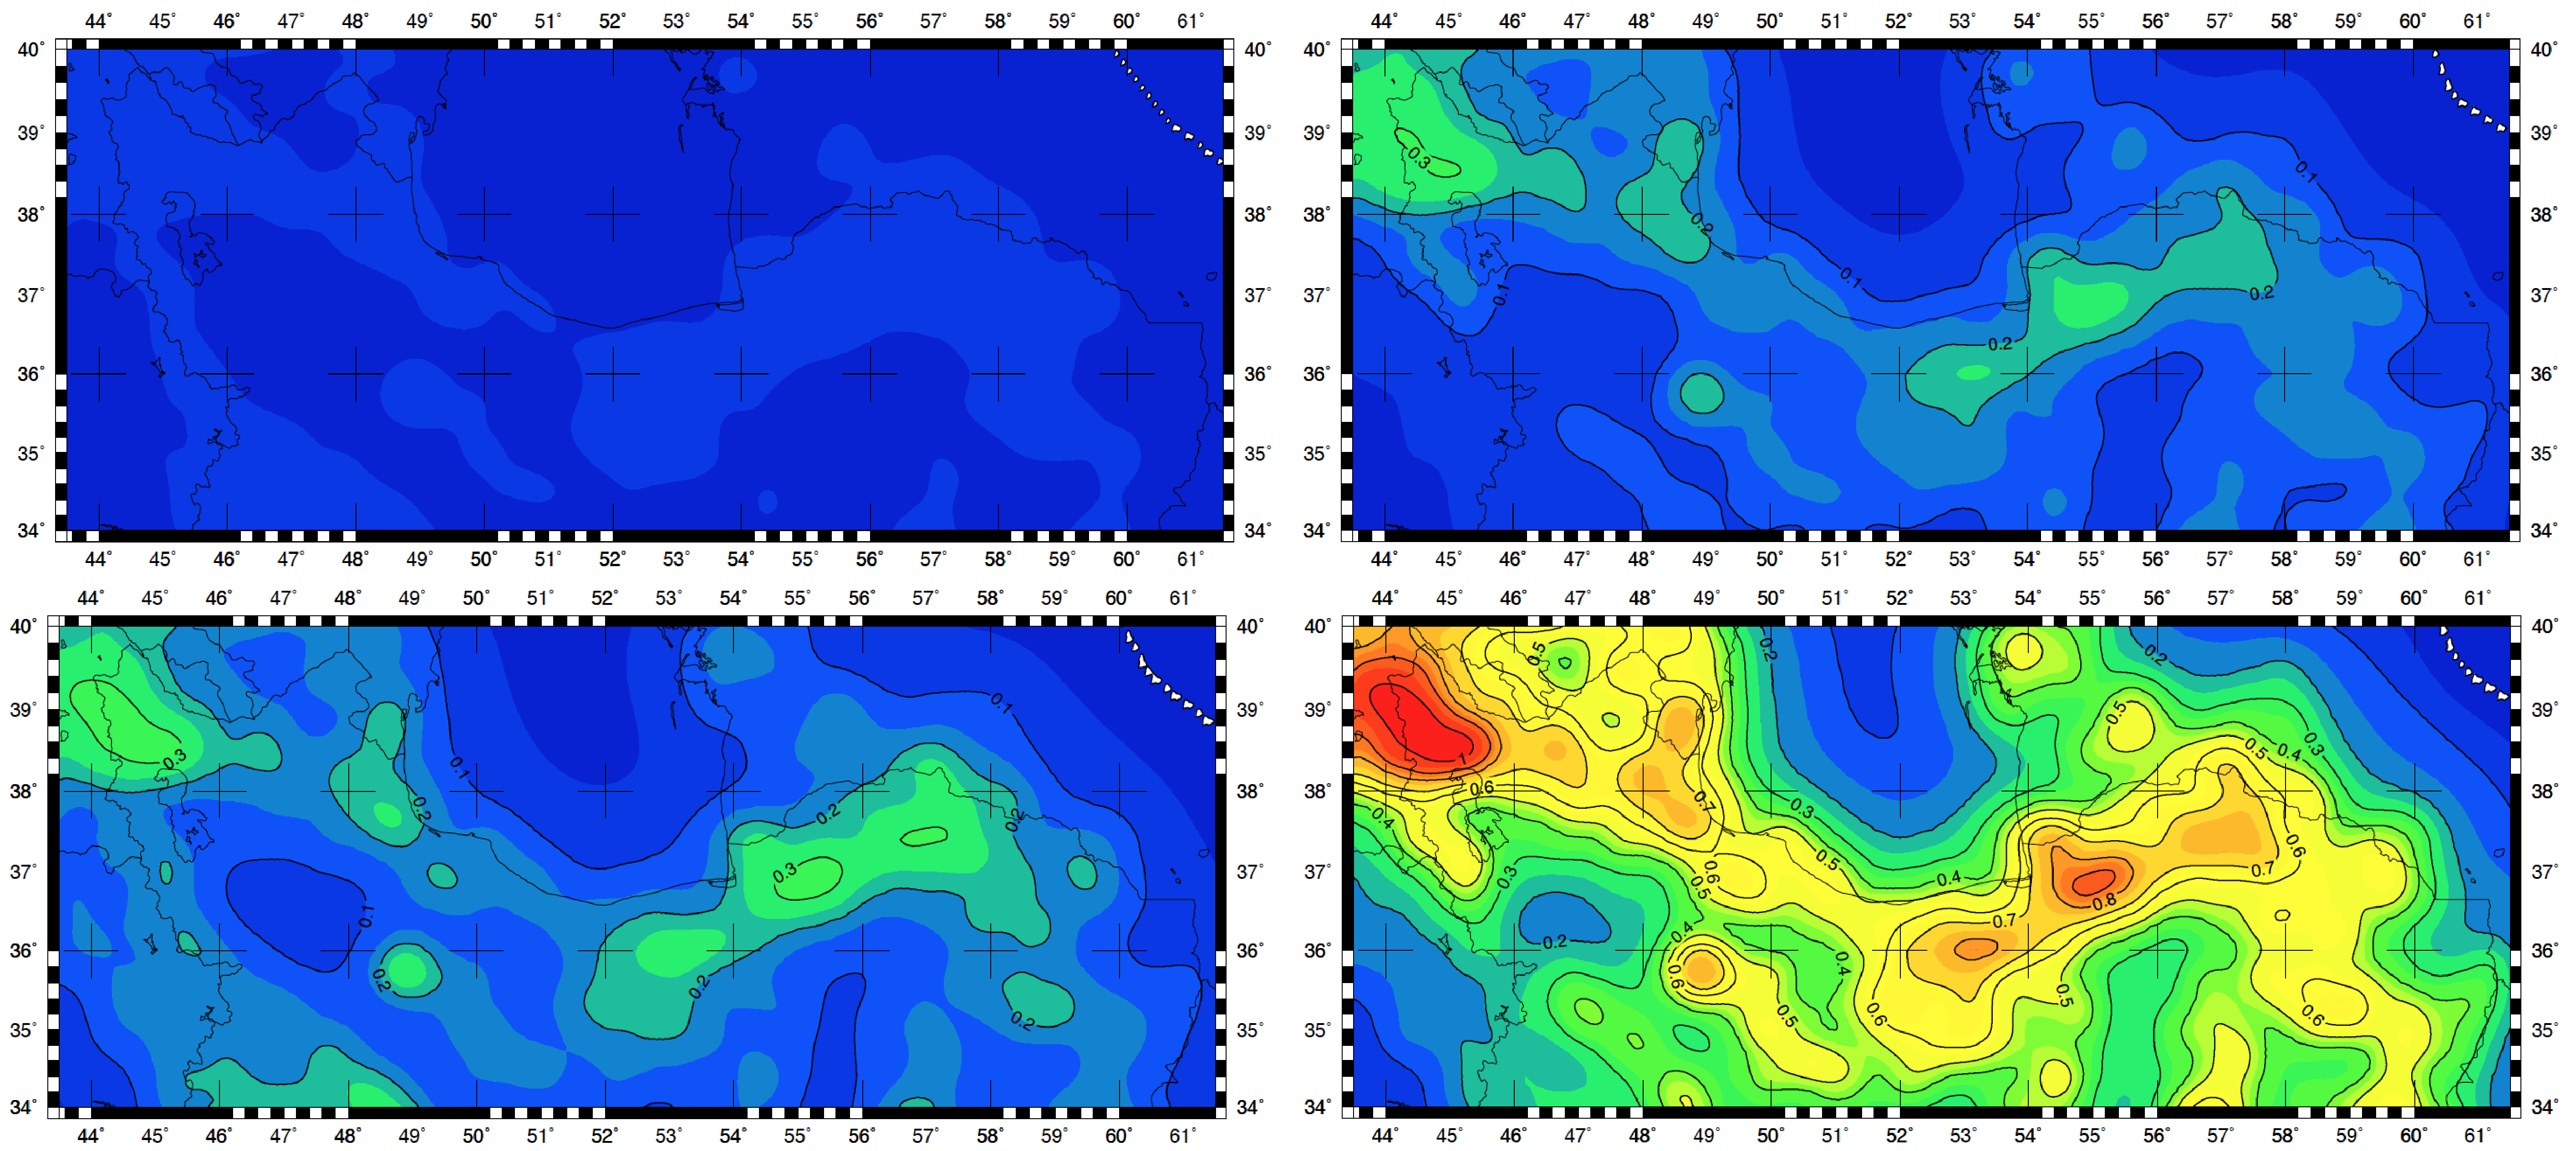
\includegraphics[scale=0.15]{figures/pdf/pga_10_minus_plus.pdf} 
% \caption{$\pm$ standard deviation of peak ground acceleration for 10\% probability of exceedance in 50 years.}
% \label{fig:pga_10_minus_plus}
% \end{figure*}


% \begin{figure*} [!ht]
% \centering
% 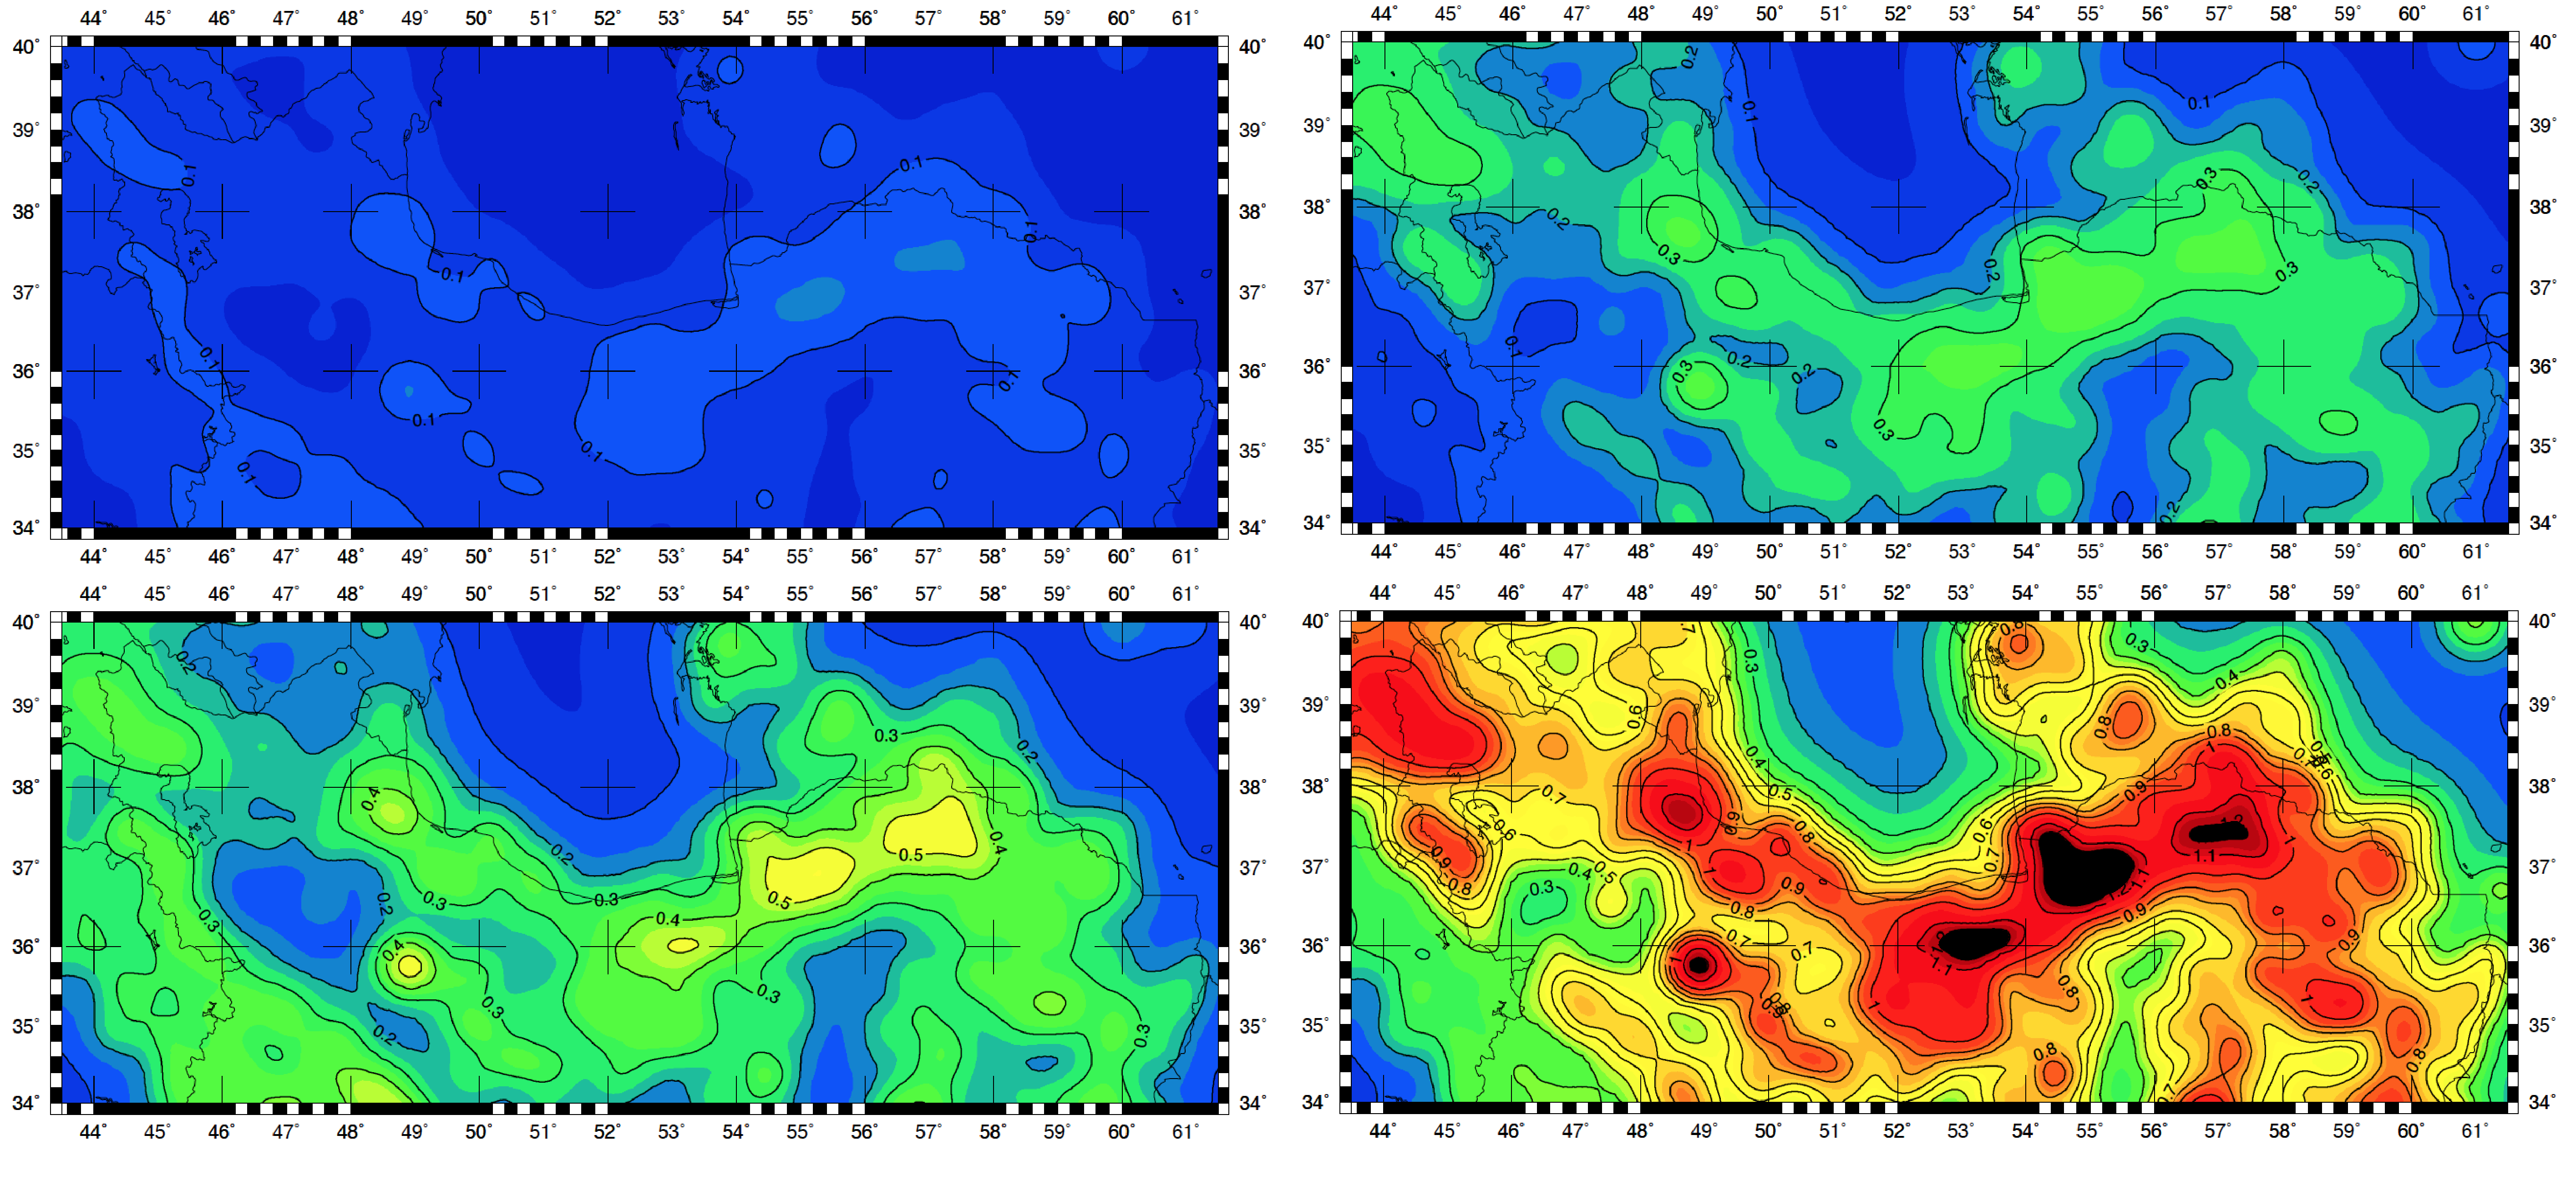
\includegraphics[scale=0.15]{figures/pdf/pga_2_minus_plus.pdf} 
% \caption{$\pm$ standard deviation of peak ground acceleration for 2\% probability of exceedance in 50 years.}
% \label{fig:pga_2_minus_plus}
% \end{figure*}



%\subsection{30-70}
%\subsection{Hazard Curve}


% \input{conclusion}    

% \section{Acknowledgements}

 We express our appreciation to Art Frankel, PhD, of the U.S. Geological Survey, Washington, DC, who kindly provided the Smoothed Probabilistic Seismic Hazard Analysis (PSHA) package. We are also very thankful to Andrzej Kijko, Director of the University of Pretoria Natural Hazard Centre, Pretoria, Africa, who generously provided the software to compute seismicity parameters. We wish to thank Mehdi Zare, International Institute of Earthquake Engineering and Seismology, Tehran, Iran, for  kindly providing the uniform historical seismic catalog. We also are very grateful to the International Institute of Earthquake Engineering and Seismology of Iran, Tehran, Iran, for providing the uniform instrumental earthquake catalog. 

 








% Bibliography
\bibliographystyle{spbasic}
\bibliography{references}
% \nocite{*}


% END: The Document
\end{document}
